%% Dissertationsvorlage
%%
%% Karlsruhe Institute of Technology
%% Institute for Program Structures and Data Organization
%% Chair for Software Design and Quality (SDQ)
%%
%% Dr.-Ing. Erik Burger
%% burger@kit.edu
%%
%% Siehe https://sdq.kastel.kit.edu/wiki/Dokumentvorlagen

% Für Dokumentoptionen siehe README.md

\documentclass[format=a4-sdq]{sdqdiss}

%% --------------------------------
%% | Font and language setup      |
%% --------------------------------

\usepackage[T1]{fontenc}
\usepackage[utf8]{inputenc} % allow utf-8 input
\usepackage[T2A,T1]{fontenc}  % use 8-bit T1 fonts, T2A Cyrillic fonts

% better looking fonts
\usepackage[tt=false, type1=true]{libertine}
\usepackage{libertinust1math}
% Improves general appearance of the text
\usepackage[protrusion=true,expansion=true,kerning]{microtype}

% set up for Japanese
\usepackage{CJKutf8}
\newcommand{\ja}[1]{\begin{CJK}{UTF8}{min}#1\end{CJK}}

% Für Sprachumschaltung
\usepackage[russian,ngerman,english]{babel}
\selectlanguage{english}

%% --------------------------------
%% | Misc setup                   |
%% --------------------------------

\usepackage{csquotes}

% Abstract
\newcommand{\Abstract}[1][Abstract]{\chapter*{#1}\addcontentsline{toc}{chapter}{#1}\markboth{#1}{#1}} 

%% Nur als Beispiel – im endgültigen Dokument bitte entfernen
\usepackage{blindtext}
% TikZ ist kein Zeichenprogramm
\usepackage{tikz}
% Schöne Tabellen
\usepackage{booktabs}
%% /Beispiel

%% --------------------------------
%% | Heading setup                |
%% --------------------------------

% Fancy chapter headings
\usepackage{quotchap}
% adjustment of header font
\makeatletter
\renewcommand*{\chapnumfont}{%
  \usefont{T1}{\@defaultcnfont}{n}{n}\fontsize{100}{130}\selectfont%
  \color{chaptergrey}%
}
\makeatother
% make headlines use serif font
\addtokomafont{disposition}{\rmfamily}

% % TODO: consider using appendix package (see msc)
% % enable appenix
% \usepackage[toc,page]{appendix}
% \noappendicestocpagenum

%% --------------------------------
%% | Bibliographie setup          |
%% --------------------------------

%% Biber statt BibTeX, siehe README.md
\usepackage[citestyle=numeric,style=numeric,backend=biber,defernumbers=true,maxnames=5]{biblatex}
\addbibresource{bib/dis.bib}
% %% Define custom sorting scheme: year (earliest first), then name, then title
% \DeclareSortingScheme{ynt}{
%   \sort[direction=ascending]{\field{year}}
%   \sort{\field{name}}
%   \sort{\field{title}}
%   \sort{\field{entrykey}}
% }
%% Define highlight based on bibtex annotation for own publications
\renewcommand*{\mkbibnamegiven}[1]{%
  \ifitemannotation{highlight}
    {\textbf{#1}}
    {#1}}

\renewcommand*{\mkbibnamefamily}[1]{%
  \ifitemannotation{highlight}
    {\textbf{#1}}
    {#1}}


%% --------------------------------
%% | Additional packages          |
%% --------------------------------

% - - - notes
% - packages NOT TO USE
%   - natbib (causes compile to fail)
% - - - /notes

\usepackage[hidelinks]{hyperref}

% - - - intro
\usepackage{fontawesome}
\usepackage[most]{tcolorbox}
\definecolor{pubgreen-box}{RGB}{112,214,167}
\definecolor{pubgreen-bg}{RGB}{247,247,244}
\definecolor{discussionpurp-box}{RGB}{181,145,180}
\definecolor{discussionpurp-bg}{RGB}{251,249,251}
\definecolor{infogrey-box}{RGB}{163,163,163}
\definecolor{infogrey-bg}{RGB}{250,250,250}
\definecolor{rqblue-box}{RGB}{103,188,223}
\definecolor{rqblue-bg}{RGB}{247,252,253}
\newtcolorbox{infobox-pub}{
    breakable,
    enhanced,
    arc=1pt,
    colback=pubgreen-bg,
    colframe=pubgreen-box,
    coltext=black,
    leftrule=36pt,
    overlay={%
     \begin{tcbclipframe}
      \node[anchor=center, xshift=19pt, yshift=-18pt, text=pubgreen-bg] at (frame.north west){\Large\faFileText};
     \end{tcbclipframe}
    }
}
\newtcolorbox{infobox-discussion}{
    breakable,
    enhanced,
    arc=1pt,
    colback=discussionpurp-bg,
    colframe=discussionpurp-box,
    coltext=black,
    leftrule=36pt,
    overlay={%
     \begin{tcbclipframe}
      \node[anchor=center, xshift=19pt, yshift=-18pt, text=discussionpurp-bg] at (frame.north west){\Large\faComments};
     \end{tcbclipframe}
    }
}
\newtcolorbox{infobox-info}{
    breakable,
    enhanced,
    arc=1pt,
    colback=infogrey-bg,
    colframe=infogrey-box,
    coltext=black,
    leftrule=36pt,
    overlay={%
     \begin{tcbclipframe}
      \node[anchor=center, xshift=19pt, yshift=-18pt, text=infogrey-bg] at (frame.north west){\Large\faInfoCircle};
     \end{tcbclipframe}
    }
}
\newtcolorbox{infobox-q}{
    breakable,
    enhanced,
    arc=1pt,
    colback=rqblue-bg,
    colframe=rqblue-box,
    coltext=black,
    leftrule=36pt,
    overlay={%
     \begin{tcbclipframe}
      \node[anchor=center, xshift=19pt, yshift=-18pt, text=rqblue-bg] at (frame.north west){\Large\faQuestionCircle};
     \end{tcbclipframe}
    }
}
%\faBookmark       -- contribution
%\faChain          -- link of some sort
%\faTag            -- note
%\faNavicon        -- general
%\faSignal         -- improvement
%\faGraduationCap  -- hypothesis?
%\faUniversity     -- sth of significance
%\faShield         -- protection
%\faGroup          -- sth w/ community?
%\faMap            -- sth w/ planning?
%\faPlus           -- mby contribution, but also looks medical
%\faThumbTack      -- slightly weird shape
% - - - /intro

% - - - corpus
\usepackage{amsmath,amssymb}
\usepackage{tabularx}
\usepackage{array}
\usepackage{threeparttable}
\usepackage{listings}
\lstset{
  basicstyle=\footnotesize\ttfamily,
  frame=single,
  breaklines=true,
  breakatwhitespace=true,
  postbreak=\space
}
\definecolor{UniBlue}{RGB}{0, 74, 153}
\definecolor{RandomRed}{RGB}{181, 93, 76}
% - - - /corpus

% - - - reference coverage and granularity (unarXive 2022)
\colorlet{listingpunct}{red!60!black}
\definecolor{listingbg}{HTML}{F7F7F7}
\definecolor{listingdelim}{RGB}{20,105,176}
\colorlet{listingcmnt}{magenta!60!black}

\lstdefinelanguage{json}{
    basicstyle=\normalfont\ttfamily,
    stepnumber=1,
    numbersep=8pt,
    showstringspaces=false,
    breaklines=true,
    frame=lines,
    backgroundcolor=\color{listingbg},
    morecomment=[s]{/*}{*/},
    commentstyle=\color{listingcmnt}\ttfamily,
    literate=
     *{:}{{{\color{listingpunct}{:}}}}{1}
      {,}{{{\color{listingpunct}{,}}}}{1}
      {\{}{{{\color{listingdelim}{\{}}}}{1}
      {\}}{{{\color{listingdelim}{\}}}}}{1}
      {[}{{{\color{listingdelim}{[}}}}{1}
      {]}{{{\color{listingdelim}{]}}}}{1},
}
\usepackage{lscape}
% - - - /reference coverage and granularity (unarXive 2022)

% - - - references accross languages
\usepackage{multirow}  % colspan/rowspan
% - - - /references accross languages

% - - - references with usage parameters
\usepackage{subfig}
\usepackage{wrapfig}
\usepackage{colortbl}
\definecolor{artifactblue}{HTML}{0059A0}
\definecolor{parametergreen}{HTML}{539A55}
\definecolor{valuered}{HTML}{CF8369}
\definecolor{contextgrey}{HTML}{A0A0A0}
\definecolor{lightgrey}{HTML}{CFCFCF}
\definecolor{listingbg}{HTML}{F7F7F7}
\definecolor{listingdelim}{RGB}{20,105,176}
\colorlet{listingcmnt}{magenta!60!black}

\lstdefinelanguage{plain}{
    stepnumber=1,
    numbersep=8pt,
    showstringspaces=false,
    breaklines=true,
    frame=lines,
    backgroundcolor=\color{listingbg},
    morecomment=[s]{/*}{*/},
    commentstyle=\color{listingcmnt}\ttfamily,
    breakindent=0pt,
}
% - - - /references with usage parameters

%% --------------------------------
%% | Title page                   |
%% --------------------------------

\title{Data Mining and Information Extraction Methods for Large-Scale High Quality Representations of Scientific Publications}
\author{Tarek Saier}
\subject{}

\subtitle{
\vskip2em
zur Erlangung des akademischen Grades eines\\[1em]
Doktors der Ingenieurwissenschaften\\
(Dr.-Ing.)\\[1em]
von der Fakultät für Wirtschaftswissenschaften\\
des Karlsruher Instituts für Technologie (KIT)\\[1em]
vorgelegte\\
Dissertation\\[1.5em]
von
}

\author{{\LARGE M.\,Sc. Tarek Saier}}

\publishers{%
\flushleft\small
\begin{align*}
    &\text{Tag der mündlichen Prüfung:} &\text{XX. Monat XXXX}\\
    &\text{Referent:} &\text{Prof. Dr. N. N.}\\
    &\text{Korreferent:} &\text{Prof. Dr. M. M.}
\end{align*}
}

\date{}  % used to supress printing a date

%% --------------------------------
%% | Document start               |
%% --------------------------------

\begin{document}
\selectlanguage{ngerman}
\maketitle

%% --------------------------------
%% | Abstract                     |
%% --------------------------------

% Römische Seitenzahlen
\frontmatter

%% Englischer Abstract
\selectlanguage{english}
\Abstract{}
% motivation
Scientific publications are written by humans \emph{for humans}.
However, vital infrastructure in academia relies on the processing of publications \emph{by computers}.
For example, academic search engines and performance indicators, which are indispensable for literature review and decision making, require machine-readable representations of publications.
Bridging the gap from a medium \emph{for humans} to something suitable for processing \emph{by computers} is a challenging and error-prone process.

% gap
Existing methods for the creation of data representing publications, and by extension the data they produce, are limited in various ways. Specifically, there are shortcomings regarding documents' interconnections, language coverage, and content representation granularity. For example, widely used data sets have highly incomplete citation networks, are limited to publications written in English, or fail to accurately capture mathematical notation. As a consequence, applications and research building on this data are of limited scope and validity.

% solution
To address these issues, we present a set of data mining and information extraction approaches that enable the creation of machine-readable publication corpora more complete, extensive, and of finer granularity than previously available. We quantify our contributions to better data quality along the dimensions relevance, accuracy, timeliness, comparability, and completeness, and achieve improvements across all of them.

In particular, we present the following.
As the foundation of our research, we introduce a method for creating a large-scale corpus of linked, full-text documents from publications' \LaTeX\ sources.
Utilizing the resulting corpus, we further present approaches yielding advances in three areas.
First, we demonstrate improvements in the completeness of citation networks though the use of a blocking and matching method, as well as improvements in the granularity of document representations.
Second, we show advances in the language coverage of document interconnections through identifying and analyzing cross-lingual citations.
Third, we present information extraction approaches for fine-granular representations of research artifacts and their parameters.

% summary
Overall, our approaches address key shortcomings of existing methods for the creation of data representing publications.
For each of our approaches, we demonstrate its viability and benefits through evaluations and practical large-scale applications.
Our methods have already been adopted in several parts of the research community, which further confirms their utility.


%% Deutsche Zusammenfassung
\selectlanguage{ngerman}
\Abstract[Zusammenfassung]{}
\Blindtext[10]


%% --------------------------------
%% | ToC                          |
%% --------------------------------

% Sprache der Dissertation
\selectlanguage{english}

\tableofcontents

% Linksbündige Einträge ohne Einzug
\listoffigures
\listoftables

%% --------------------------------
%% | Content                      |
%% --------------------------------

% Arabische Seitenzahlen
\mainmatter

\chapter{Introduction}
\label{chp:introduction}

% What do I want to say and convey here?
% - scientific publications are the ``footprint'' and ``medium of discourse'' of academic progress
% - structured representation

% establish the nature and role of scientific publications
Scientific publications are the \emph{discourse medium} and \emph{literary footprint} of academic progress. As such, they play a vital role in the everyday workings and advancement of academia.
% segue to the digital
Historically, this role manifested itself physically---through ink on paper. In time, digital methods for authoring %/composition?
and distribution enabled more efficient ways of dissemination.
Today, scientific publications are predominantly authored, distributed, consumed, and archived digitally~\cite{Lamers2018}. However, the form of today's digital publications still retains numerous and deep traces of its physical ancestry.

% Digital dissemination makes the transfer of new knowledge into the research community faster and cheaper. Digital archives enable search technology and analytics to operate on our \emph{literary footprint} of past and present academic progress. In this way, digitization facilitates both faster progress in science, \emph{and} technology helping scientists to keep up with the increase in speed. However, today's form of digital publications is far from optimal for powering such technology. In fact, the form of today's digital publications poses significant challenges for 

% While there lies enormous potential in a digital record of science, there remain significant challenges to realizing this potential. A key cause of these challenges is the historical baggage of today's digital publications. This dissertation is in pursuit of tackling these challenges.

% There lies enormous potential in a digital record of science. But realizing this potential

The historical baggage manifesting itself in the PDF files we read, share, and author, poses significant challenges to realizing the full potential of a digital record of science. While digital services in academia such as search and recommendation do exist, they are powered not by publications themselves, but rather by more structured, derivative representations of publications. The same holds for analyses of publications. The creation of such structured representations %/derivates?
is challenging and error prone, leading to a risk of subpar services and erroneous analyses. This dissertation represents and effort to tackle this challenge and alleviate the quality of structured representations of scientific publications.

% (random alliteration: structured surrogates of academic archives)

% - b/c of discrepancy between current form and what would be even better for digital dissemination and use (e.g. more structured), structured derivates of publications that enable digital services are of limited quality
% - historical baggage in part b/c still meant for human consumption
% - gap(?) between “pure” digital form and current form hinders more efficient use in digital services surrounding publications and academia

\section{Motivation}

% What do I want to say and convey here?
% - why do we have/need scholarly data?
% - in contrast to intro paragraphs above, make *necessity* of scholarly data for mitigating information overload clear
% - also make clear why there was realistic potential in approaching the challenge

In the following, we discuss the importance of structured representations of scientific publications---from hereon referred to as ``scholarly data'' for the sake of legibility%
\footnote{Note that in other contexts the term ``scholarly data'' can have a broader meaning than just ``structured representations of scientific publications''. For example, it can also include data on research institutions or funding bodies, without necessitating the context of a publication.}%
---, and based on that derive the motivation of the research project.

Digitization in academia, and with it the inception of scholarly data, has enabled an acceleration of scientific progress. Digital dissemination makes the transfer of new knowledge into the research community faster% as well as cheaper
, and digital archives enable search technology and analytics to operate on large collections of publications. A second factor for acceleration is increased research spending across the world~\cite{CRS2022,OECD2023}. An increase in scientific progress, and with that an increase in the rate at which research results are published, also means a growing challenge for researchers to keep up.

While ...
% * in the olden days there were polymaths
% * nowadays an expert can't humanly keep up with their field
% * → we need assistance
% * → my research in on enabling the creating of such assistance

% * since ever, humans have sought shortcuts
% * in decision making in science: h-imdex etc. (not sure if this fits b/c I don't specifically address such metrics)

% * not only is my research addressing the now pressing and increasing issue of an increasing rate of publication
% * it also tackles blind spots the have been left unaddressed for long (x-ling)



% big picture view on bridging the gap between historical baggage documents (print, scan, PDF, ...) and digital representation
% - large existing current effort
%       - document image dewarping
%       - OCR
%       - PDF based scholarly data stuff


%Measuring the Evolution of a Scientific Field through Citation Frames~~\cite{Jurgens2018} (usable here (or in HyperPIE chapter) for extra justification of focus on parameters of used artifacts)

\begin{infobox-pub}
\textbf{Publication} \fullcite{Saier2020}
\end{infobox-pub}

\begin{infobox-discussion}
\textbf{Discussion} This text should show what a printed text will look like at this place. If you read this text, you will get no information. Really? Is there no information?
\end{infobox-discussion}

\begin{infobox-info}
\textbf{Remark} This text should show what a printed text will look like at this place. If you read this text, you will get no information. Really? Is there no information?
\end{infobox-info}

\begin{infobox-q}
\textbf{RQ1} How can the completeness of the citation network in scholarly data sets be improved?
\end{infobox-q}

\begin{infobox-progress}
      \begin{tabular}{ccl}
        \toprule
        Crit.\tnote{a} & Res.\tnote{b} & Explanation \\
        \midrule
        \textbf{C1} & {\large\textbf{+}} & Representative coverage in physics, mathematics, CS \\
        \textbf{C2} & $\circ$ & Primary focus on text content \\
        \textbf{C3} & {\large\textbf{+}} & $>96$\% accuracy in reference matching \\
        \textbf{C4} & {\large\textbf{+}} & Low noise due to using \LaTeX\ as data source \\
        \textbf{C5} & {\large\textbf{+}} & Publications until end of most recent full year \\
        \textbf{C6} & {\large\textbf{+}} & Provides MAG and arXiv IDs; DOIs in linked MAG \\
        \textbf{C7} & $\circ$ & Not considered at this stage \\
        \textbf{C8} & {\large\textbf{+}} & 42.6\% reference matching success rate \\
        \textbf{C9} & {\large\textbf{+}} & Full-text included \\
        \bottomrule
      \end{tabular}
\end{infobox-progress}

\section{Research Questions}

Research questions are provided as a guidance to the reader, giving a high-level perspective on the insights provided by the publications making up this dissertation.
% RQ "formulas":
% Q: "How can <goal> be achieved? A: "<proposed method>"
% Q: "How can <proposed method aspect> be leveraged to achieve <goal>? A: "<proposed method>"
% Q: "What's the nature of <analysis object>?" A: "<analysis result>

\section{Contributions}

\begin{table}[tb]
\centering
  \caption{Overview of publications reused in this dissertation.}
  \label{tab:primarypublicationoverview}
  \begin{tabular}{cllllclr}
    \hline
    \ & \ & \ & \ & \ & Author & Venue & \ \\
    Chap. & Venue & Year & Type & Length & Position & Rating & Ref. \\
    \hline
    3 & Scientometrics & 2020 & Journal & Full & 1 of 2 & SJR Q1 & \cite{Saier2020} \\
    \arrayrulecolor{lightgrey}\cline{1-8}
    \multirow{2}{*}{4} & JCDL & 2022 & Workshop & Full & 1 of 3 & Core A* & \cite{Saier2022ULITE} \\
    \ & JCDL & 2023 & Conference & Short & 1 of 3 & Core A* & \cite{Saier2023unarXive} \\
    \arrayrulecolor{lightgrey}\cline{1-8}
    \multirow{2}{*}{5} & ICADL & 2020 & Conference & Full & 1 of 2 & Core A & \cite{Saier2020xling} \\
    \ & IJDL & 2022 & Journal & Full & 1 of 3 & SJR Q2 & \cite{Saier2021} \\
    \arrayrulecolor{lightgrey}\cline{1-8}\arrayrulecolor{black}
    6 & ECIR & 2023 & Conference & Full & 1 of 4 & Core A & \cite{Saier2023hyperpie} \\
    \hline
    \end{tabular}
\end{table}

The contributions in this dissertation have been published in peer-reviewed international conferences and journals. Table~\ref{tab:primarypublicationoverview} gives an overview of the publications and the chapters they make up. Venue ranks are taken from Core\refurl{http://portal.core.edu.au/conf-ranks/}{2023-10-12} in the case of conferences and from SJR\refurl{https://www.scimagojr.com/}{2023-10-12} in the case of journals.\footnote{The ranks shown are the rating for the respective publication year, or the most up-to-date ranking if the latter is not listed. For workshops, the rank of the conference at which the workshop is hosted is shown.} For each of the publications, detailed author contributions according to the Contributor Roles Taxonomy\refurl{https://credit.niso.org/}{2023-10-12} are listed at the end of the respective section.

\begin{table}[tb]
\centering
  \caption{Overview of secondary publications not reused in this dissertation.}
  \label{tab:secondarypublicationoverview}
  \begin{tabular}{llllclr}
    \hline
    \ & \ & \ & \ & Author & Venue & \ \\
    Venue & Year & Type & Length & Position & Rating & Ref. \\
    \hline
    ECIR & 2019 & Workshop & Full & 1 of 2 & Core A & \cite{Saier2019} \\
    ECIR & 2020 & Conference & Full & 1 of 3 & Core A & \cite{Saier2020a} \\
    NAACL & 2021 & Workshop & Short & 3 of 4 & Core A & \cite{Krause2021} \\
    AAAI & 2022 & Workshop & Full & 2 of 3 & Core A* & \cite{Shapiro2022} \\
    ECIR & 2022 & Workshop & Full & 4 of 5 & Core A & \cite{Faerber2022bir} \\
    JCDL & 2022 & Conference & Full & 3 of 3 & Core A* & \cite{Nishioka2022} \\
    JCDL & 2023 & Conference & Short & 1 of 3 & Core A* & \cite{Saier2023cocon} \\
    \hline
    \end{tabular}
\end{table}

Additional publications (co-)authored leading up to and during the research period which are not a direct part of this dissertation, but nevertheless informed the overall research trajectory, are listed in Table~\ref{tab:secondarypublicationoverview}. Especially \cite{Saier2019} and \cite{Krause2021}, which constitute the results of the master's thesis preceding the doctoral research period, paved the way for this dissertation.

\section{Outline}
\Blindtext[1]

% unarXive
% |  |  |
% |  |  v
% |  |  blocking
% |  v
% |  unarXive22
% v       |
% xling   v
% |      Hyperpie
% v
% xling+

\chapter{Foundations}

\section{Foo}
\Blindtext[1]

\chapter{Corpus}
\label{chp:corpus}

This chapter is based on the following publication.

\begin{infobox-pub}
\fullcite{Saier2020}
\end{infobox-pub}
\vspace{-0.5em}
\begin{footnotesize}
\textit{Remark on the connection to previous work:}
\vspace{-0.5em}
\begin{quote}
The publication cited above is a journal article that represents an extension of a previously published workshop paper~\cite{Saier2019} (see also Table~\ref{tab:secondarypublicationoverview}). For the journal article, the underlying work, writing, and publication were conducted within the doctoral research period. The preceding workshop paper reports on a result of the master's thesis before the doctoral research period (see also Section~\ref{sec:intro-puboverview}). Later in this chapter, at the end of Section~\ref{sec:related-work}, further details regarding the nature of the extension are provided.
\end{quote}
\end{footnotesize}

The work in this chapter addresses the following research task.

\begin{rtlist}
    \item \textit{Base Methodology} - establish a base methodology for generating a large-scale, high-quality scholarly data set, that is on par with or improving upon existing data sets.
\end{rtlist}

It furthermore makes contributions to the following research task, which is likewise addressed in the next chapter.

\begin{rtlist}
    \item[\rtmark{2}:] \textit{Citation Network Completeness} - develop a method to link literature references, that is able to link more references than are linked in existing data sets, while not compromising on link correctness or processing efficiency.
\end{rtlist}

\section{Overview}
In this chapter, we introduce a methodology for creating a large-scale corpus of linked, full-text documents from \LaTeX{} source files. The resulting corpus, \emph{unarXive}, comprises over one million documents across multiple scientific disciplines, and spans 27 years. It is further on also used as the basis for the research presented in the subsequent chapters. Along with the corpus creation methodology, extensive analyses of the resulting corpus are presented.

At the end of the chapter, in Section~\ref{sec:corpus-assessment}, we assess the achievement of the research tasks, as well as the contributions made in terms of the overarching research goal of enabling higher-quality scholarly data.

% \begin{abstract}
% In recent years, scholarly data sets have been used for various purposes, such as paper recommendation, citation recommendation, citation context analysis, and citation context-based document summarization. 
% The evaluation of approaches to such tasks and their applicability in real-world scenarios heavily depend on the used data set. However, existing scholarly data sets are limited in several regards. 
% In this paper, we propose a new data set based on all publications from all scientific disciplines available on arXiv.org. Apart from providing the papers' plain text, in-text citations were annotated via global identifiers. Furthermore, citing and cited publications were linked to the Microsoft Academic Graph, providing access to rich metadata. Our data set consists of over one million documents and 29.2 million citation contexts. The data set, which is made freely available for research purposes, not only can enhance the future evaluation of research paper-based and citation context-based approaches, but also serve as a basis for new ways to analyze in-text citations, as we show prototypically in this chapter.
% \end{abstract}

\section{Introduction}
A variety of approaches exist that utilize scientific paper collections to help researchers in their work. 
Research paper recommender systems, for example, suggest relevant papers to read~\cite{Beel2016fixed}. Other systems operate on a more fine-grained level within the full-text of papers, such as the textual contexts in which citations appear (``citation contexts''). 
Based on citation contexts, things like the citation function~\cite{Teufel2006EMNLP,Teufel2006fixed,Moravcsik1975}, the citation polarity~\cite{GhoshD017,Abujbara2013}, and the citation importance~\cite{Valenzuela2015fixed,Chakraborty2016} can be determined. Furthermore, citation contexts are necessary for context-aware citation recommendation~\cite{He2010WWW,Ebensu2017}, as well as for citation-based document summarization tasks~\cite{Chandrasekaran2019}, such as citation-based automated survey generation~\cite{Mohammad2009} and automated related work section generation~\cite{Jinggiang2007}.

The evaluation of approaches developed for all these tasks, as well as the actual applicability and usefulness of developed systems in real-world scenarios, heavily depend on the data that is used. This typically is a collection of papers provided as full-text, or a set of already extracted citation contexts, consisting of, for instance, 1--3 sentences each. Existing data sets, however, are limited in various ways (see Section~\ref{sec:related-work} for more details):

\begin{enumerate}
 \item[(1)] \textit{Size.} Data sets can be comparatively small (fewer than 100,000 documents), which makes them difficult to use for training and testing machine learning approaches.
 \item[(2)] \textit{Cleanliness.} Papers' full-texts or citation contexts are often very noisy due to the conversion from PDF to plain text and due to encoding issues.
 \item[(3)] \textit{Global citation annotations.} Links from citations in the text to the structured representations of the cited publications across documents are often not provided.
 \item[(4)] \textit{Data set interlinkage.} For citing and cited documents, data sets often do not provide identifiers from widely used bibliographic databases, such as DBLP\refurl{https://dblp.uni-trier.de/}{2023-11-06} or the Microsoft Academic Graph (MAG).\refurl{https://www.microsoft.com/en-us/research/project/microsoft-academic-graph/}{2023-11-06}
 \item[(5)] \textit{Cross-domain coverage.} Often, only documents from a single scientific discipline are included, restricting the coverage of evaluations and applications based on the data set.
\end{enumerate}

To address these limitations, we propose a new scholarly data set, which we call \emph{unarXive}.\footnote{The name is derived from the name of the data source, \textit{arXiv}, and the verb \textit{to unarchive}, indicating the extraction of files from an archive.} The data set comprises papers' full-text, a citation network, and additional metadata.
It is freely available at \refurlinline{http://doi.org/10.5281/zenodo.3385851}{2023-11-06} and the implementation for creating it at \refurlinline{https://github.com/IllDepence/unarXive}{2023-11-06}.

\begin{table}[t]
\centering
  \caption[Overview of the proposed data set]{Overview of the proposed data set.}
  \label{tbl:allthestats}
\begin{small}
\begin{tabular}{lrcc|cc}
\toprule
    \ & \ & citing & \ & \ & cited \\
    \ & \ & documents & \multicolumn{2}{c}{references} & documents \\
    \ & \ & \  & \tiny{outgoing} & \tiny{incoming} & \  \\
    \emph{full data set:} & \ & \textbf{1,043,126} & 15,954,664 & 15,954,664 & \textbf{2,746,288} \\
    &\tiny{full-text}&\tiny{1,043,126}&\tiny{15,954,664}&\tiny{7,181,576}&\tiny{736,597}\\
    &\tiny{linked to MAG}&\tiny{994,351}&\tiny{15,846,351}&\tiny{15,954,664}&\tiny{2,746,288}\\
    \emph{by discipline:} & \ & \ & \ & \ & \ \\
    \multicolumn{2}{r}{physics} & 662,894 & 9,300,576 & 7,827,072 & 921,852 \\
    \multicolumn{2}{r}{mathematics} & 237,422 & 3,426,117 & 5,062,033 & 906,301 \\
    \multicolumn{2}{r}{computer science} & 111,694 & 2,526,656 & 1,876,401 & 425,860 \\
    \multicolumn{2}{r}{other} & 31,116 & 701,315 & 1,189,158 & 492,275 \\
  \bottomrule
    \\
    \multicolumn{6}{l}{
        \begin{tabular}{rl}
            \textbf{data}: & \refurlinline{http://doi.org/10.5281/zenodo.3385851}{2023-11-06} \\
            \textbf{code}: & \refurlinline{https://github.com/IllDepence/unarXive}{2023-11-06} \\
        \end{tabular}
        }
\end{tabular}
\end{small}
\end{table}

Table~\ref{tbl:allthestats} gives an overview of the proposed data set. Note that throughout this chapter, we refer to links between publications on the \emph{document level} as ``references'' (corresponding to entries in a section ``bibliography'' or ``references'' near the end of a document), whereas on the \emph{text level}, we speak of ``citations'' (indicated by markers within the text associated with a reference). The proposed data set consists of over one million full-text documents (about 269 million sentences) and links to 2.7 million unique publications via 15.9 million unique references and 29.2 million citations.
Thus, we argue that it is considerably large, addressing limitation~(1). By using publications' \LaTeX{} source files and developing a highly accurate transformation method that converts \LaTeX{} to plain text, we can resolve issue~(2). Besides the pure papers' content, in-text citations are annotated directly in the text via global identifiers, thereby covering aspect~(3). As far as possible, (citing and cited) documents are linked to the Microsoft Academic Graph~\cite{Sinha2015} addressing limitation item~(4). This enables us to use the arXiv paper content in combination with the metadata in the MAG, which, as of February 2019, contains data on 213 million publications along with metadata about researchers, venues, and fields of study. Our data set also resolves issue~(5), as all disciplines covered in arXiv are included. This enables researchers to analyze papers from several disciplines and to compare approaches using scholarly data across disciplines.

% Aspect/benefit #1:
Considering the application of our data set, we argue that it not only can be used as a new large data set for evaluating paper-based and citation-based approaches with unlimited citation context lengths (since the publications' full-text is available),
% Aspect/benefit #2:
but also be a basis for novel ways of paper analytics within bibliometrics and scientometrics. For instance, based on the citation contexts and the citing and cited papers' metadata in the MAG, analyses on biases in the writing and citing behavior of researchers---e.g.\ related to authors' affiliation~\cite{Reingewertz2018} or documents' language~\cite{Liang2013,Liu2018}---can be performed.
%% Aspect/benefit #3:
Furthermore, deep learning approaches, which have been widely used in the digital library domain recently~\cite{Ebensu2017}, require huge amounts of training data. Our data set allows to overcome this hurdle and investigate how far deep learning approaches can lead us.
% overall
Overall, we argue that with our data set we can significantly bring the state of the art of big scholarly data one step forward.

We make the following contributions in this chapter:
\begin{enumerate}
    \item We propose a large, interlinked scholarly data set with papers' full-text, annotated in-text citations, and links to rich metadata. We describe its creation process in detail and provide both the data as well as the creation process implementation to the public. 
    \item We manually evaluate the validity of our reference links on a sample of 300 references, thereby providing insight into our citation network's quality.
    \item We calculate statistical key figures and analyze the data set with respect to its contained references and citations.
    \item We compare our reference links to those in the MAG, and manually evaluate the validity of links only appearing in either of the data sets. In doing so, we identify a large number of documents where the MAG lacks coverage.
    \item We analyze the likelihood with which in-text citations in our data set refer to specific parts of a cited document depending on the discipline of the citing \emph{and} cited document. Such an analysis is only possible with word level precision citation marker positions annotated in full-text \emph{and} metadata on citing as well as cited documents. The analysis therefore can showcase the practicability of our data set.
\end{enumerate}

The remainder of the chapter is structured as follows: After outlining related data sets in Section~\ref{sec:related-work}, we describe our data set creation method in Section~\ref{sec:data-set-creation}. This is followed by statistics and key figures in Section~\ref{sec:statistics}. In Section~\ref{sec:evaluation-validity-and-coverage}, we evaluate the validity and coverage of our reference links. Section~\ref{sec:analysis} is dedicated to the analysis of citation flow and citation contexts. We conclude with a summary and an outlook in Section~\ref{sec:conclusion}, and an overarching result assessment in Section~\ref{sec:corpus-assessment}.

\section{Existing Data Sets}
\label{sec:related-work}

Table~\ref{tab:existing-data-sets} gives an overview of related data sets.
CiteSeerX can be regarded as the most frequently used evaluation data set for citation-based tasks.
For our investigation, we use the snapshot of the entire CiteSeerX data set as of October 2013, published by~\cite{Huang2015fixed}. This data set consists of 1,017,457 papers, together with 10,760,318 automatically extracted citation contexts.
This data set has the following drawbacks~\cite{Roy2016fixed,Faerber2018LREC}: The provided meta-information about cited publications is often not accurate. Citing and cited documents are not interlinked to other data sets. Moreover, the citation contexts can contain noise from non-ASCII characters, formulas, section titles, missed references and/or other ``unrelated'' references, and do not begin with a complete word.

\begin{table}[tb]
 % \caption{Overview of existing data sets\\\small{(\#P.=Number of papers; Cit.\ cont.=Citation contexts; Ref.\ IDs=Reference IDs; CS=Computer Science, BM=Biomedicine, LS=Life Sciences, CL=Computer Linguistics)\\(\emph{extractable*} indicates that extraction might be error-prone due to papers only being available in PDF format)}}
 % NOTE: above is original caption, but does not compile in this document class
 \caption[Overview of existing data sets]{Overview of existing data sets (\#Papers=Number of papers; Cit.\ contexts=Citation contexts; CS=Computer Science, BM=Biomedicine, LS=Life Sciences, CL=Computer Linguistics; extractable* indicates that extraction might be error-prone due to papers only being available in PDF format).}
 \label{tab:existing-data-sets}
  \centering
  \begin{small}
 \begin{threeparttable}
 \begin{tabular}{llllll}
 \toprule
   Data set & \#\,Papers & Cit. contexts & Scope & Full text & Reference IDs \\
   \midrule
   % capital Ms and lowercase ks (supposed to be like that)
   CiteSeerX~\cite{Caragea2014}/RefSeer~\cite{Huang2015fixed} &  1.0\,M & 400 characters & (all) & no & no \\
   PMC OAS\tnote{a} & 2.3\,M & extractable & BM/LS & yes & mixed \\
   Scholarly Dataset 2~\cite{Sugiyama2015} & 0.1\,M & extractable* & CS & yes & no \\
   arXiv CS~\cite{Faerber2018LREC}   &  0.09\,M & 1 sentence & CS & yes & DBLP \\
   ACL-ARC~\cite{Bird2008ACLARC} & 0.01\,M & extractable* & CS/CL & yes & no \\
   ACL-AAN~\cite{Radev2013} & 0.02\,M & extractable* & CS/CL & yes & no  \\
   \bottomrule
 \end{tabular}
 \begin{tablenotes}
    \item[a] See \refurlinline{https://www.ncbi.nlm.nih.gov/pmc/tools/openftlist/}{2023-11-06}.
  \end{tablenotes}
\end{threeparttable}
  \end{small}
\end{table}

The PubMed Central Open Access Subset (PMC OAS) is another large data set that has been used for citation-based tasks~\cite{Gipp2015,Duma2016,Galke2018}. Contained publications are already processed and available in the JATS~\cite{Huh2014} XML format. While the data set overall is comparatively clean, heterogeneous annotation of citations within the text and mixed usage of identifiers of cited documents (PubMed, MEDLINE, DOI, etc.) make it difficult to retrieve high-quality citation interlinkings of documents from the data set\footnote{To be more precise, the heterogeneity makes the usage of the data set \emph{as is} unfeasible. Resolving references to a single consistent set of identifiers retroactively would be an option, but comparatively challenging in the case of PubMed, because of the frequent usage of special notation in publication titles; see also: \refurlinline{https://zenodo.org/records/3598421/files/CITREC_Parser_Documentation.pdf}{2023-11-06}.}~\cite{Gipp2015}.

Beside the aforementioned, there are other collections of scientific publications. Among them are the ACL Anthology corpus~\cite{Bird2008ACLARC} and Scholarly Dataset 2~\cite{Sugiyama2015}.
Note that these data sets only contain the publications themselves, typically in PDF format. Therefore, using such data sets for paper-based or citation-based approaches is troublesome, since one must preprocess the data (i.e., (1) extract the content without introducing too much noise, (2) specify global identifiers for cited papers, and (3) annotate citations with those identifiers).
Furthermore, there are data sets for evaluating paper recommendation tasks, such as CiteULike\refurl{https://web.archive.org/web/20190211033621/http://www.citeulike.org/faq/data.adp}{2023-11-06} or Mendeley,\refurl{https://data.mendeley.com/}{2023-11-06}. These, however, only provide metadata about publications or are not freely available for research purposes.

F{\"{a}}rber et al.\ also published a data set with annotated arXiv papers' content in the past~\cite{Faerber2018LREC}. In comparison, our data set is superior to it in the following regards:
\begin{enumerate}
    \item[(1)] Our data set is considerably larger (1 M instead of 90 k documents).
    \item[(2)] Our data set ensures cleanliness of the papers' full-text and citation contexts by using a more feature rich conversion pipeline.
    \item[(3)] We develop a new method for resolving references to consistent global identifiers. Contrary to the method in~\cite{Faerber2018LREC}, we evaluate our method and thereby demonstrate its performance (see Section~\ref{sec:evaluation-reference-resolution}).
    \item[(4)] While~\cite{Faerber2018LREC} link documents solely to DBLP, which covers computer science papers, our data set links documents to the Microsoft Academic Graph, which covers all scientific disciplines and which has been used frequently in the digital library domain in recent years~\cite{Mohapatra2019}.
    \item[(5)] While the data set in~\cite{Faerber2018LREC} is restricted to computer science, the new data set covers all domains of arXiv (see Section~\ref{sec:statistics} and Figure~\ref{fig:sankey}).
\end{enumerate}

Lastly, compared to a preliminary version of our data set~\cite{Saier2019}, the data we present here has been improved in several ways. Most notably, while in the initial version, only citing papers were associated with arXiv identifiers and only cited papers had been linked to the MAG, we now provide both types of IDs for both sides. This means, that for nearly all documents, MAG metadata is easily accessible, and full-text is not only available for all citing papers but now also for over a quarter of the cited papers. Moreover, we provide significantly more details and insights into the data set's creation process (see Section~\ref{sec:data-set-creation}) and its resulting characteristics (see Sections~\ref{sec:evaluation-validity-and-coverage} and \ref{sec:analysis}).



\section{Data Set Creation}
\label{sec:data-set-creation}

Scientific publications are usually distributed in formats targeted at \emph{human consumption} (e.g., PDF) or, in cases like arXiv, also as source files the aforementioned (e.g., \LaTeX{} sources for generating PDFs). Citation-based tasks, such as context-aware citation recommendation, in contrast, require \emph{automated processing} of the publications' textual contents as well as the documents' interlinking through in-text citations. The creation of a data set for such tasks therefore encompasses two main steps: extraction of plain text and resolution of references. In the following, we will describe how we approached these two steps using arXiv publications' \LaTeX{} sources and the Microsoft Academic Graph.

\subsection{Used Data Sources}
The following two resources are the basis of the data set creation process.

\paragraph{arXiv} hosts over 1.5 million documents from August 1991 onward.%
\refurl{https://arxiv.org/stats/monthly_submissions}{2023-11-06} They are available not only as PDF, but (in most cases) also as \LaTeX{} source files. The discipline most prominently represented is physics, followed by mathematics, with computer science seeing a continued increase in percentage of submissions ranking third (see Figure~\ref{fig:sankey}). The availability of \LaTeX{} sources makes arXiv documents particularly well suited for extracting high-quality plain text and accurate citation information. So much so, that it has been used to generate ground truths for the evaluation of PDF-to-text conversion tools~\cite{Bast2017}.
\paragraph{Microsoft Academic Graph} is a very large, automatically generated data set on 213 million publications, related entities (authors, venues, etc.), and their interconnections through 1.4 billion references.\footnote{Numbers as of February 2019.} It has been widely used as a repository of all publications in academia in the fields of bibliometrics and scientometrics~\cite{Mohapatra2019}. While pre-extracted citing sentences are available, these do not contain annotated citation marker positions. Full text documents are also not available. The size of the MAG makes it a good target for matching reference strings\footnote{I.e., the entries in the reference section of a publication. See Listing~\ref{lst:refitems} for examples.} against it, especially given that arXiv spans several disciplines.

\subsection{Pipeline Overview}

\begin{figure}[tb]
  \centering
    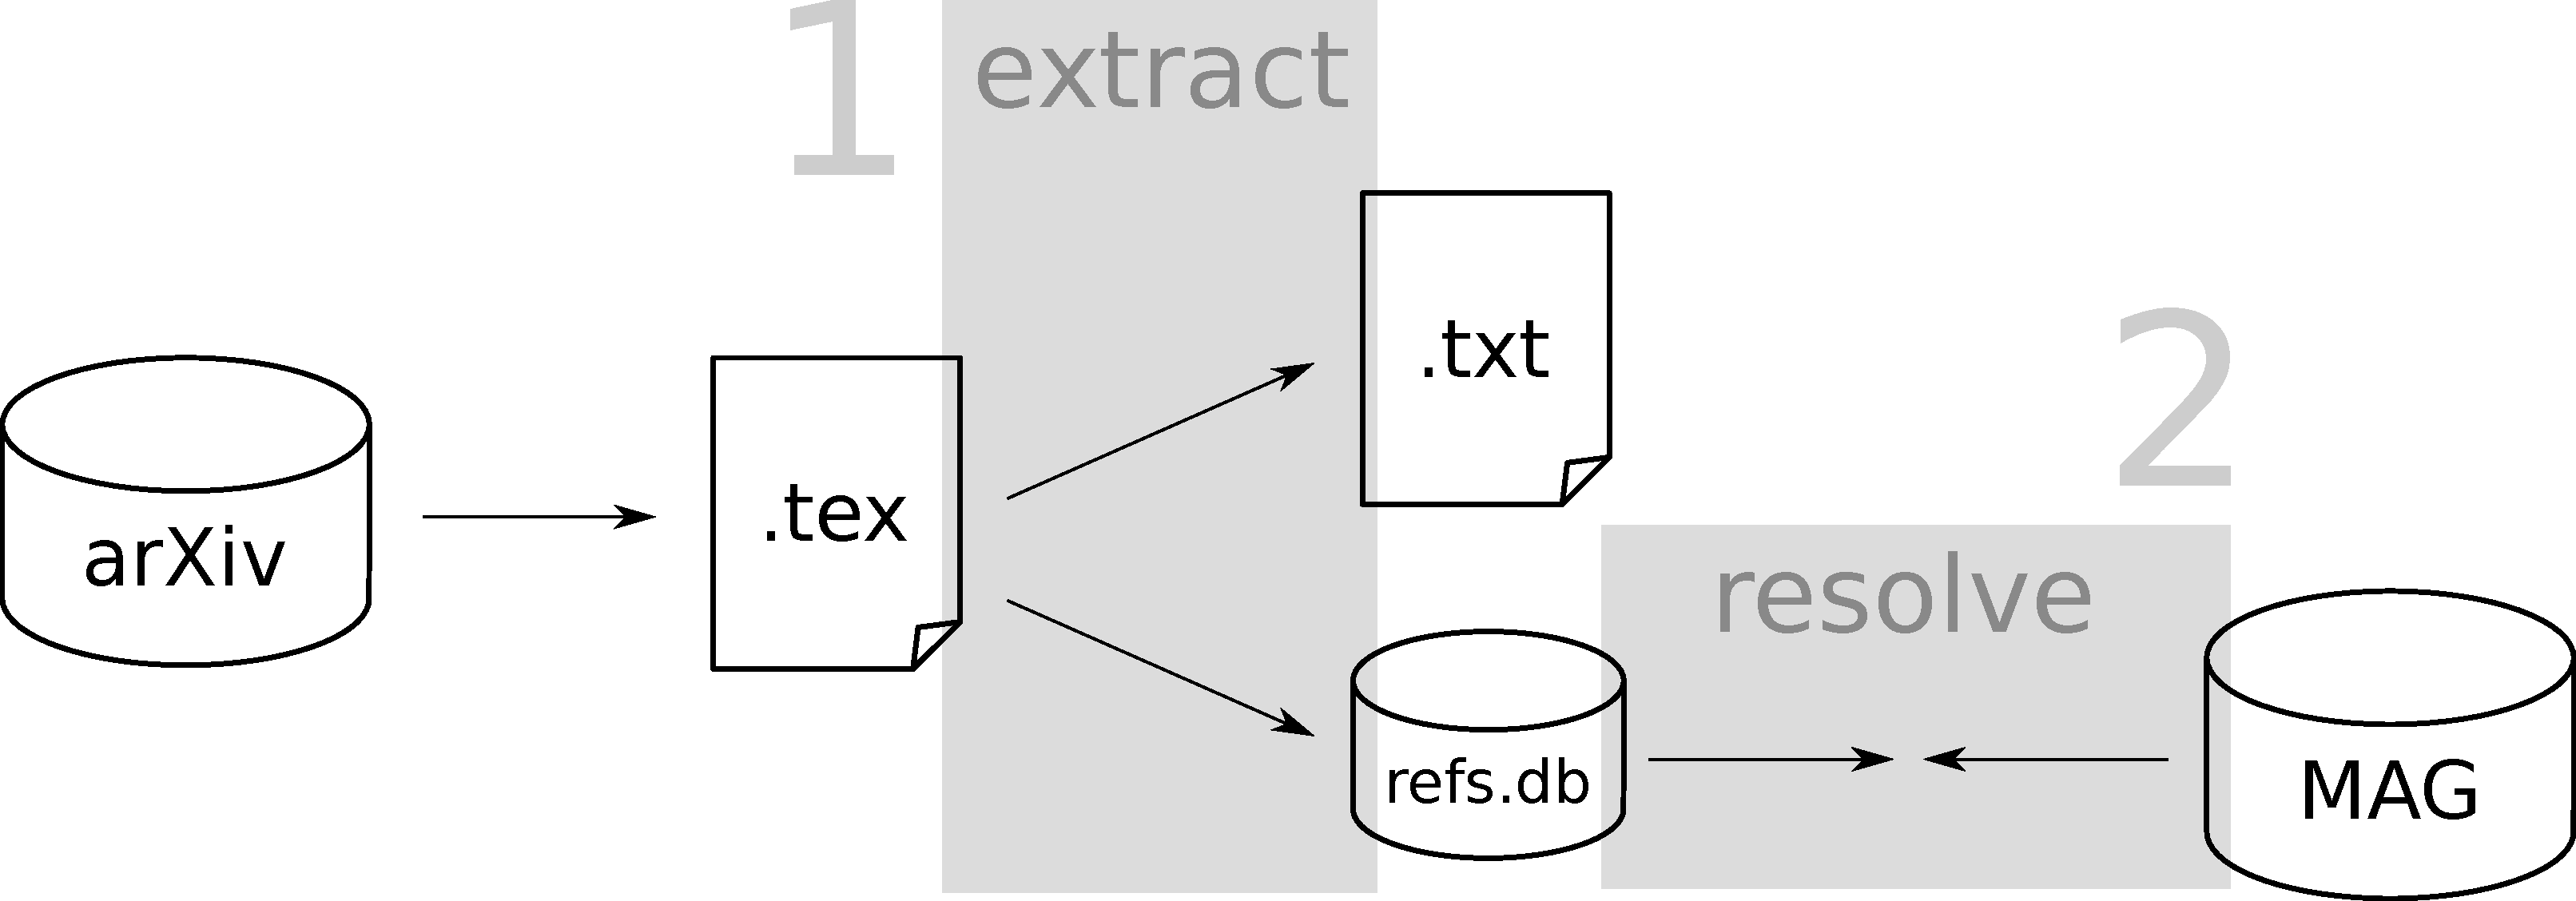
\includegraphics[width=.7\textwidth]{figures/corpus/Fig1.pdf}
  \caption[Schematic representation of the data set generation process]{Schematic representation of the data set generation process.}
  \label{fig:datagen}
\end{figure}

To create the data set, we start out with arXiv sources (see Figure~\ref{fig:datagen}). From these we generate, per publication, a plain text file with the document's textual contents and a set of database entries reflecting the document's reference section. Association between reference strings and in-text citation locations are preserved by placing citation markers in the text. In a second step, we then iterate through all reference strings in the database and match them against paper metadata records in the MAG. This gives us full-text arXiv papers with (word level precision) citation links to MAG paper IDs. As a final step, we enrich the data with MAG IDs on the citing paper side (in addition to the already present arXiv IDs) and arXiv IDs on the cited paper side (in addition to the already present MAG IDs)---this is a straightforward process, because the paper metadata in the MAG includes source URLs, meaning papers found on arXiv have an arXiv.org source URL associated with them, such that a mapping from arXiv IDs to MAG IDs can be created.

Listing~\ref{lst:formatall} shows how our data set looks like. In the following, we describe the main steps of the data set creation process in more detail.

\subsection{\LaTeX{} Parsing}
In the following, we will describe the tools considered for parsing \LaTeX{}, the challenges we faced in general and with regard to arXiv sources in particular, and our resulting approach.

\subsubsection{Tools}

\begin{table}[tb]
\centering
  \caption[Comparison of tools for parsing \LaTeX{}]{Comparison of tools for parsing \LaTeX{}.}
  \label{tbl:tools}
\begin{small}
\begin{threeparttable}
\begin{tabular}{llll}
\toprule
    Tool & Output & Robust & Usable as is \\
   \midrule
    plastex\tnote{a} & DOM & no & yes\\
    TexSoup\tnote{b} & document tree & no & yes\\
    opendetex\tnote{c}\,/detex\tnote{d} & plain text & no & yes\\
    GrabCite~\cite{Faerber2018LREC} & plain\hphantom{ }text\hphantom{ }+ resolved ref. & yes & no\\
    \LaTeXML{}\tnote{e} & XML & yes & yes\\
    Tralics\tnote{f} & XML & yes & yes\\
  \bottomrule
\end{tabular}  \begin{tablenotes}
    \item[a] See \refurlinline{https://github.com/tiarno/plastex}{2023-11-06}.
    \item[b] See \refurlinline{https://github.com/alvinwan/texsoup}{2023-11-06}.
    \item[c] See \refurlinline{https://github.com/pkubowicz/opendetex}{2023-11-06}.
    \item[d] See \refurlinline{https://www.freebsd.org/cgi/man.cgi?query=detex}{2023-11-06}.
    \item[e] See \refurlinline{https://github.com/brucemiller/LaTeXML}{2023-11-06}.
    \item[f] See \refurlinline{https://www-sop.inria.fr/marelle/tralics/}{2023-11-06}.
  \end{tablenotes}
\end{threeparttable}
\end{small}
\end{table}

We took several tools for a direct conversion from \LaTeX{} to plain text or to intermediate formats into consideration and evaluated them. Table~\ref{tbl:tools} gives an overview of our results. Half of the tools failed to produce any output for a large amount of arXiv documents we used as test input and were therefore deemed not robust enough. \textit{GrabCite}~\cite{Faerber2018LREC} is able to parse 78.5\%
of arXiv CS documents but integrates resolving references (see Section~\ref{sec:refresol}) against DBLP into the parsing process and therefore would require significant modification to fit our new system architecture. \textit{\LaTeXML{}} and \textit{Tralics} are both robust and can be used as \LaTeX{} conversion tools as is. Based on subsequent tests, we observed that \textit{LaTeXML} needs on average 7.7 seconds (3.3 if formula environments are heuristically removed beforehand) to parse an arXiv paper, while \textit{Tralics} needs 0.09. Because the quality of their output seemed comparable, we chose to use \textit{Tralics}.

\subsubsection{Challenges}\label{sec:refresolchallenges}
Apart from the general difficulty of parsing \LaTeX{} due to its feature richness and people's free-spirited use of it, we especially note difficulty in dealing with extra packages not included in documents' sources.\footnote{The arXiv guidelines specifically suggest the omission of such (see \refurlinline{https://arxiv.org/help/submit_tex\#wegotem}{2023-11-06}).} While \textit{Tralics}, for example, is supposed to deal with \textit{natbib} citations,\refurl{https://www-sop.inria.fr/marelle/tralics/packages.html\#natbib}{2023-11-06} normalization of such citations leads to a decrease of citation markers not being able to be matched to an entry in the document's reference section from 30\% to 5\% in a sample of 565,613 citations we tested.

\subsubsection{Resulting Approach}
Our \LaTeX{} parsing solution consists of three steps: flattening, parsing, and output generation. First, we flatten each arXiv document's sources to a single \LaTeX{} file using \textit{latexpand}\refurl{https://ctan.org/pkg/latexpand}{2023-11-06}\textsuperscript{,}\footnote{We also tested flatex (\refurlinline{https://ctan.org/pkg/flatex}{2023-11-06}) and flap (\refurlinline{https://github.com/fchauvel/flap}{2023-11-06}) but got the best results with latexpand.} and normalize citation commands (e.g.\ \texttt{\textbackslash citep*}, \texttt{\textbackslash citet[see]}, \texttt{\textbackslash citealt}, etc. to \texttt{\textbackslash cite}) to prevent parsing problems later on. In the second step, we then generate an XML representation of the \LaTeX{} document using \textit{Tralics}. Lastly, we go through the generated XML structure and produce two types of output---(i)~an annotated plain text file with the document's textual contents and (ii)~database entries reflecting the document's reference section. For (i) we replace XML nodes that represent formulas, figures, tables, as well as intra-document references with replacement tokens and turn XML nodes originating from citation markers in the \LaTeX{} source (i.e., \texttt{\textbackslash cite}) into plain text citation annotation markers. For (ii), each entry in the document's reference section is assigned a unique identifier, its text is stored in a database, and the identifier put into the corresponding annotation in the plain text (see Listing~\ref{lst:formatall}).

\subsection{Reference Resolution}
\label{sec:refresol}
Resolving references to globally consistent identifiers (e.g.\ detecting that the reference strings (1), (2), and (3) in Listing~\ref{lst:refitems} all reference the same document) is a challenging and still unsolved task~\cite{Nasar2018}. Given it is the most distinctive singular part of a publication, we base our reference resolution on the title of the cited work and use other pieces of information (e.g., the authors' names) only in secondary steps. In the following, we will describe the challenges we faced, matching arXiv documents' reference strings against MAG paper records, and how we approached the task.

\subsubsection{Challenges}
Reference resolution can be challenging when reference strings contain only minimal amounts of information, when formulas or other special notation is used in titles, or when they refer to non publications (e.g., Listing~\ref{lst:refitems}, (4)--(6)).  Another problem we encountered was noise in the MAG. One such case are the MAG papers with IDs \texttt{2167727518} and \texttt{2763160969}. Both are identically titled \emph{``Observation of a new boson at a mass of 125 GeV with the CMS experiment at the LHC''} and dated to the year 2012. But while the former is cited 17k times and cites 112 papers within the MAG, the latter is a neither cited nor cites any other papers.\footnote{The MAG record with ID \texttt{2763160969} appears to be a noisy duplicate caused by a web source with easily misinterpretable author information (only a partial list is displayed).} Taking the number of citations into account when matching references, reduced the number of mismatches in this particular case from 2,918 to 0 and improved the overall quality of matches in general.

\begin{lstlisting}[caption={Examples of reference strings.},label={lst:refitems}]
(1) V. N. Senoguz and Q. Shafi, arXiv:hep-ph/0412102
(2) V.N. Senoguz and Q. Shafi, Phys. Rev. D 71 (2005) 043514.
(3) V. N. Senoguz and Q. Shafi, ''Reheat temperature in supersymme
    tric hybrid inflation models,'' Phys. Rev. D 71, 043514 (2005)
     [hep-ph/0412102].
(4) V.Sauli, JHEP 02, 001 (2003).
(5) Aaij, Roel, et al. "Search for the $B^{0}_{s} \to \eta^{\prime
    }\phi$ decay" Journal of High Energy Physics 2017.5 (2017): 15
    8.
(6) According to the numerous discussions with my colleagues <remo
    ved> and <removed> an experimental verification of our theoret
    ical predictions is feasible.
\end{lstlisting}

\subsubsection{Resulting Approach}
Our reference resolution procedure can be broken down in two steps: title identification and matching. If contained in the reference string, title identification is performed based on an arXiv ID or DOI (where we retrieve the title from an arXiv metadata dump or via crossref.org\refurl{https://www.crossref.org/}{2023-11-06}); otherwise we use Neural ParsCit~\cite{neuralparscit}.\footnote{For title identification we also considered two other state of the art~\cite{Tkaczyk2018} tools, namely CERMINE~\cite{Tkaczyk2015} and GROBID~\cite{Lopez2009}. However, we found CERMINE to be considerably slower than the other tools. And while GROBID showed comparable speed and output quality in preliminary tests, Neural ParsCit's tag based output format was more straightforward to integrate than the faceted TEI format structures that GROBID's reference parser module returns.}
The identified title is then matched against the normalized titles of all publications in the MAG. Resulting candidates are considered, if at least one of the author's names (as given in the MAG) is present in the reference string. If multiple candidates remain, we judge by the citation count given in the MAG---this particularly helps mitigate matches to rouge almost-duplicate entries in the MAG, which often have few to no citations, like paper \texttt{2763160969} mentioned in the previous section.

\subsection{Result format}
Listing~\ref{lst:formatall} shows some example content from the data set. In addition to the paper plain text files and the references database, we also provide the citation contexts of all successfully resolved references extracted to a CSV file as well as a script to create custom exports.\footnote{See Python script \texttt{extract\_contexts.py} bundled with the data set for details.} For the provided CSV export, we set the citation context length to 3 sentences---the sentence containing the citation as well as the one before and after---as used by~\cite{Tang2014} and~\cite{Huang2015fixed}. Each line in an export CSV has the following columns: cited MAG ID, adjacent cited MAG IDs, citing MAG ID, cited arXiv ID, adjacent cited arXiv IDs, citing arXiv ID, text (see bottom of Listing~\ref{lst:formatall}). Citations are deemed adjacent, if they are part of a citation group or are at most 5 characters apart (e.g.\ ``\emph{[27,42]''}, \emph{``[27], [42]''} or \emph{``[27] and [42]''}). The IDs of adjacent cited documents are added, because those documents are cited in an almost identical context (i.e., only a few characters to the left or right).
% Sentence tokenization for the extraction is performed with NLTK's pre-trained PunktSentenceTokenizer.

\begin{lstlisting}[caption={Excerpts from (top to bottom) a paper's plain text, corresponding entries in the references database, entries in the MAG, and extracted citation context CSV.},label={lst:formatall}]
It has over 79 million images stored at the resolution of FORMULA 
. Each image is labeled with one of the 75,062 non-abstract nouns 
in English, as listed in the Wordnet{{cite:9ad20b7d-87d1-47f5-aeed
-10a1cf89a2e2}}{{cite: 298db7f5-9ebb-4e98-9ecf-0bdda28a42cb}} lexi
cal database.
------------------------------------------------------------------
[uuid]         [citing..] [cited..]   ...  [reference_string]
9ad20b7d-87d1  1412.3684  2081580037  ...  George A. Miller (1995)
-47f5-aeed-..                              . WordNet: A Lexical ..
298db7f5-9ebb  1412.3684  2038721957  ...  Christiane Fellbaum (19
-4e98-9ecf-..                              98), ""WordNet: An El..
------------------------------------------------------------------
[paperid]   [originaltitle]                           [publ..]  ..
2038721957  WordNet : an electronic lexical database  MIT Press ..
2081580037  WordNet: a lexical database for English   ACM       ..
------------------------------------------------------------------
2131463865|2038721957|2081580037|1412.3684|||It has over 79 millio
n images stored at the resolution of FORMULA . Each image is label
ed with one of the 75,062 non-abstract nouns in English, as listed
 in the Wordnet CIT MAINCIT lexical database. It has been noted th
at many of the labels are not reliable CIT .
\end{lstlisting}

\section{Statistics and Key Figures}
\label{sec:statistics}

In this section we present the data set and its creation process in terms of numbers. Furthermore, insight into the distribution of references and citation contexts is given.

\subsection{Creation Process}
We used an arXiv source dump containing all documents up until the end of 2018 (1,492,923 documents). 114,827 of these were only available in PDF format, leaving 1,378,096 sources. Our pipeline output 1,283,584 (93.1\%) plain text files, 1,139,790 (82.7\%) of which contained citation markers. The number of reference strings identified is 39,694,083, for which 63,633,427 citation markers were placed within the plain text files. This first part of the process took 67 hours to run, unparallelized on an 8 core Intel Core i7-7700 3.60GHz machine with 64 GB of memory.

Of the 39,694,083 reference strings, we were able to match 16,926,159 (42.64\%) to MAG paper records. For 31.32\% of the reference strings we could neither find an arXiv ID or DOI, nor was Neural ParsCit able to identify a title.\footnote{To assess whether or not the large percentage of reference strings without identified title is due to Neural ParsCit missing a lot of them, we manually check its output for a random sample of 100 papers (4027 reference strings). We find that 99\% of cases with no title identified actually do not contain a title---like for example items (1), (2) and (4) in Listing~\ref{lst:refitems}. These kinds of references seem to be most common in physics papers. The 1\% where a title was missed were largely references to non-English titles and books. We therefore conclude that the observed numbers largely reflect the actual state of reference strings rather than problems with the approach taken.} For the remaining 26.04\% a title was identified, but could not be matched to the MAG.
Of the matched 16.9 million items' titles, 52.60\% were identified via Neural ParsCit, 28.31\% by DOI and 19.09\% by arXiv ID. Of the identified DOIs, 32.9\% were found as is, while 67.1\% were heuristically determined. This was possible because the DOIs of articles in journals of the American Physical Society follow predictable patterns. The matching process took 119 hours, run in 10 parallel processes on a 64 core Intel Xeon Gold 6130 2.10GHz machine with 500 GB of memory.

Comparing the performance of our approach using all papers (1991--2018) to using only the papers from 2018 (i.e., recent content), we note that the percentage of successfully extracted plain texts goes up from 93.1 to 95.9\% (82.7 to 87.8\% only counting plain text files containing citation markers) and the percentage of successfully resolved references increases from 42.64 to 59.39\%. A possible explanation for the latter would be, that there is more and higher quality metadata coverage (MAG, crossref.org, etc.) of more recent publications.

\begin{figure}[!ht]
  \centering
  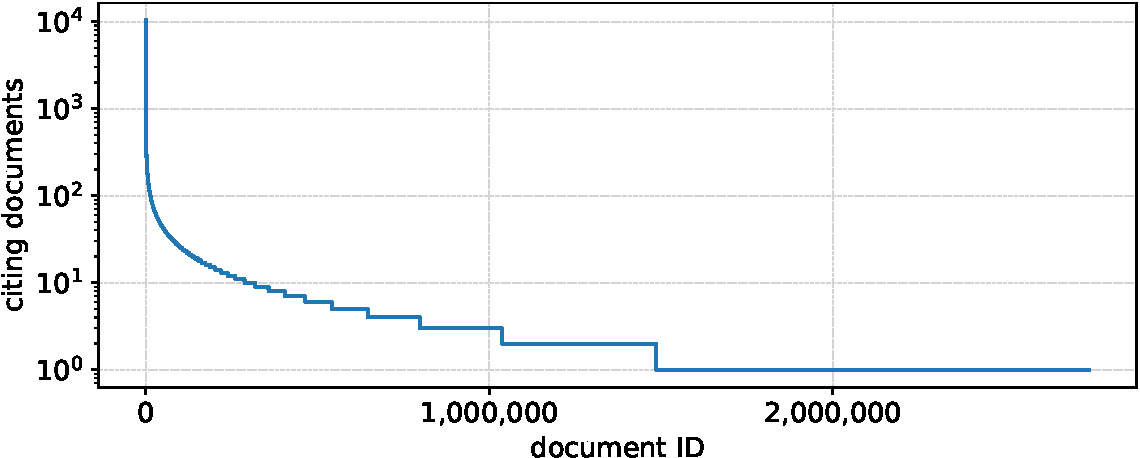
\includegraphics[width=0.92\linewidth]{figures/corpus/Fig2.pdf}
  \caption[Number of citing documents per cited document]{Number of citing documents per cited document.}
  \label{fig:numcitdoc}
  \vspace{1em}
%\end{figure}
%\begin{figure}[ht]
%  \centering
  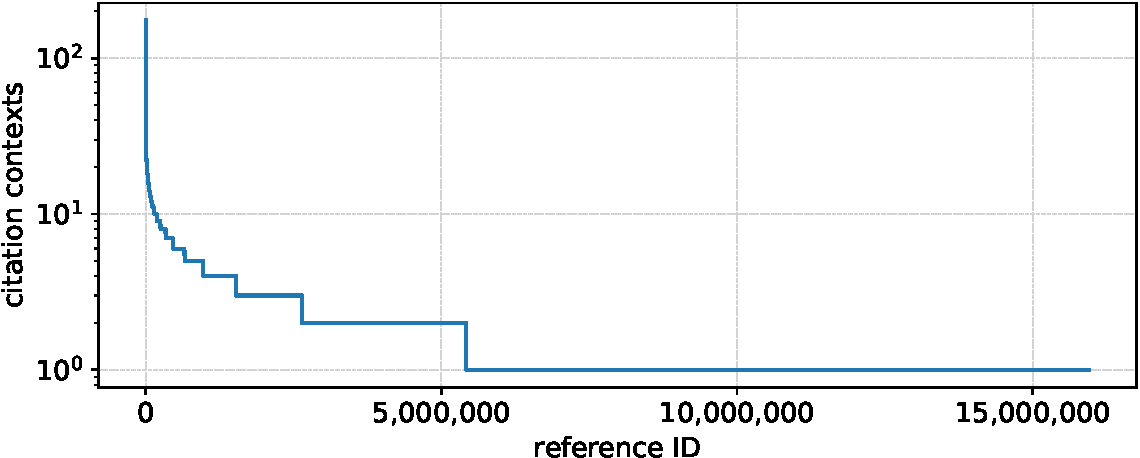
\includegraphics[width=0.92\linewidth]{figures/corpus/Fig3.pdf}
  \caption[Number of citation contexts per reference]{Number of citation contexts per reference.}
  \label{fig:numcontref}
    \vspace{1em}
\end{figure}

\subsection{Resulting Data Set}
Our data set consists of \emph{2,746,288 cited papers, 1,043,126 citing papers, 15,954,664 references and 29,203,190 citation contexts}.\footnote{References that were successfully matched to a MAG record but have no associated citation markers (due to parsing errors; see Section~\ref{sec:refresolchallenges}) are not counted here.} 
% DB entry figures (not excluding cases where no marker is present):
% cited: 2,820,381
% citing: 1,192,097
% references: 16,802,498

\begin{figure}[tb]
  \centering
    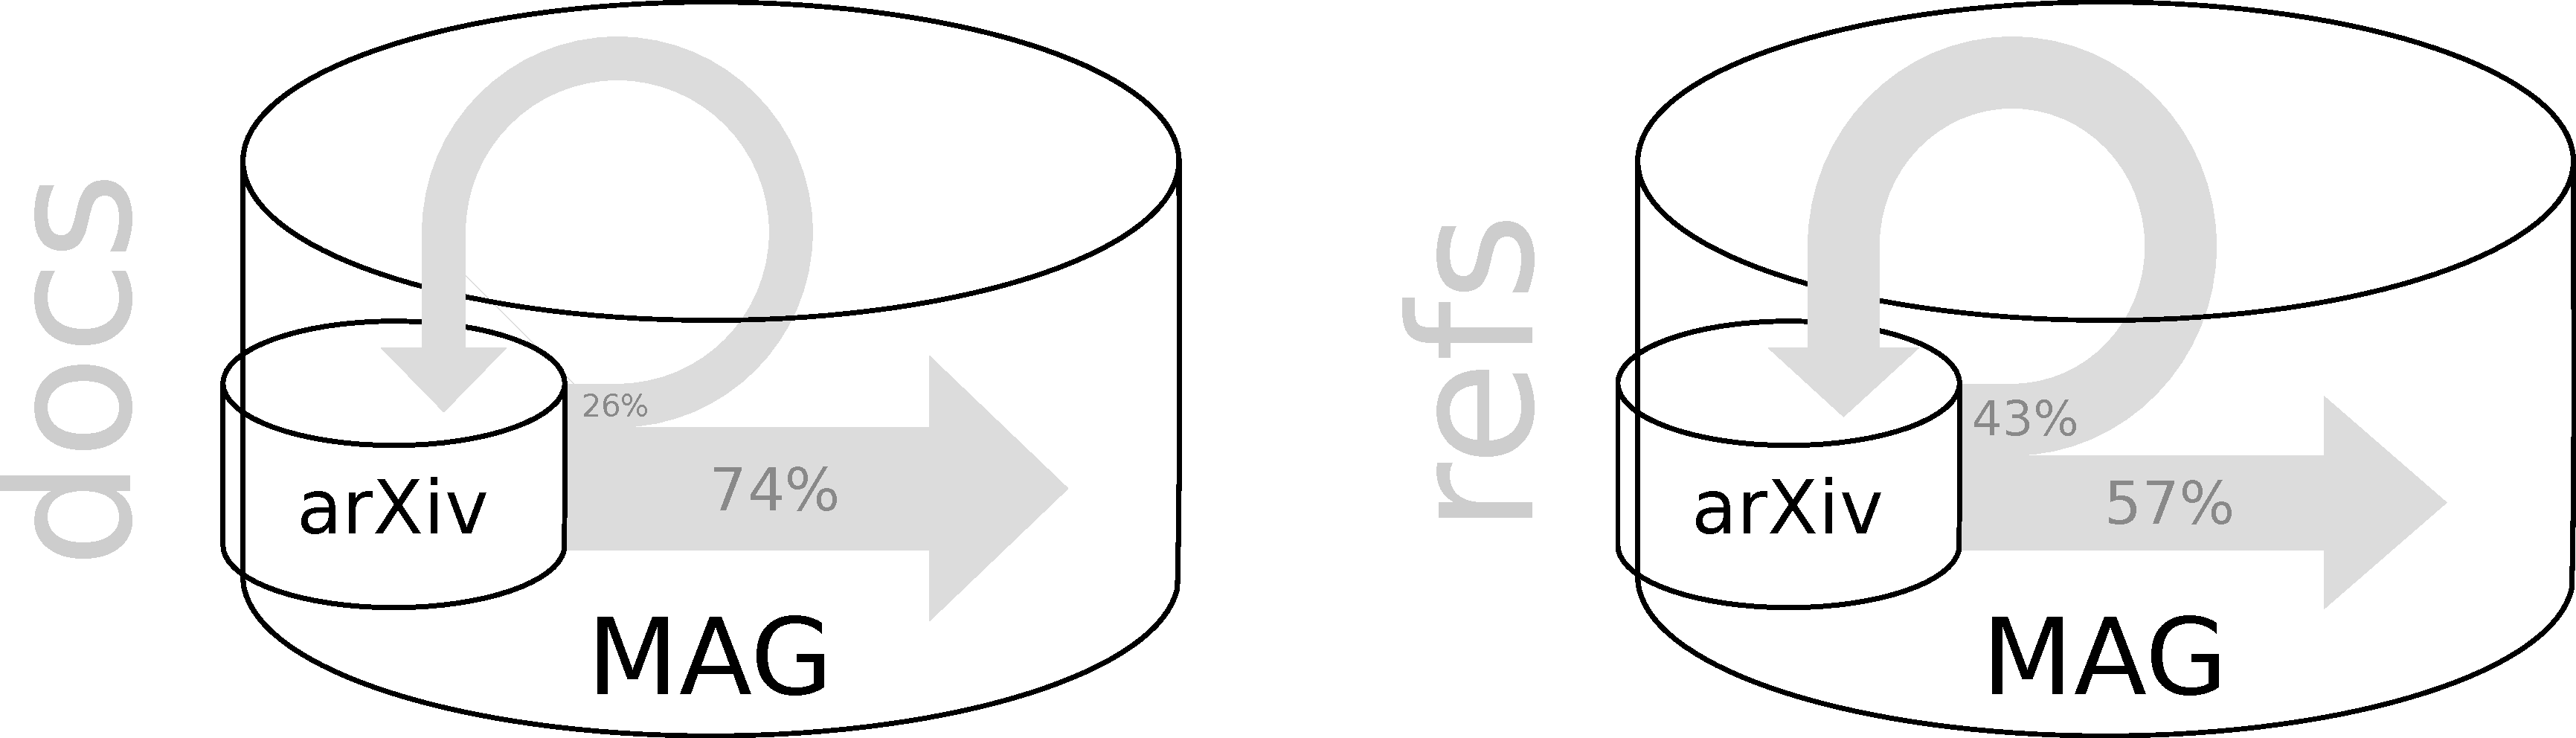
\includegraphics[width=.9\textwidth]{figures/corpus/Fig4.pdf}
  \caption[Visualization of the citation flow in terms of documents and references from arXiv to the MAG]{Visualization of the citation flow in terms of documents and references from arXiv to the MAG.}
  \label{fig:inflow}
\end{figure}

Figure~\ref{fig:numcitdoc} shows the number of citing documents for all cited documents. There is one cited document with over 10,000 citing documents, another 8 with more than 5,000 and another 14 with more than 3,000. 1,485,074 (54.07\%) of the cited documents are cited at least two times, 646,509 (23.54\%) at least five times. The mean number of citing documents per cited document is 5.81 (SD 28.51). Figure~\ref{fig:numcontref} shows the number of citation contexts per entry in a document's reference section. 10,537,235 (66.04\%) entries have only one citation context, the maximum is 278, the mean 1.83 (SD 2.00).

Because not all documents referenced by arXiv papers are hosted on arXiv itself, we additionally visualize the citation flow with respect to the MAG in Figure~\ref{fig:inflow}. 95\% of our citing documents are contained in the MAG. Of the cited documents, 26\% are contained in arXiv and therefore included as full-text, while 74\% are only included as MAG IDs. On the level of references, this distribution shifts to 43/57. The high percentages of citation links contained within the data set can be explained due to the fact, that in physics and mathematics---which make up a large part of the data set---it is common to self-archive papers on arXiv.

\section{Evaluation of Citation Data Validity and Coverage}
\label{sec:evaluation-validity-and-coverage}

\subsection{Citation Data Validity}
\label{sec:evaluation-reference-resolution}
To evaluate the validity of our reference resolution results, we take a random sample of 300 matched reference strings and manually check for each of them, if the correct record in the MAG was identified. This is done by viewing the reference string next to the matched MAG record and verifying, if the former actually refers to the latter.\footnote{Further details can be found at \refurlinline{https://github.com/IllDepence/unarXive/tree/legacy_2020/doc/matching_evaluation}{2023-11-06}.} Given the 300 items, we observed 3 errors, giving us an accuracy estimate of 96\% at the worst, as shown in Table~\ref{tbl:confvals}. Table~\ref{tbl:mismatches} shows the three incorrectly identified documents. In all three cases the misidentified document's title is contained in the correct document's title, and there is a large or complete author overlap between correct and actual match. This shows that authors sometimes title follow-up work very similarly, which leads too hard to distinguish cases.

\begin{table}[tb]
  \caption[Confidence intervals for a sample size of 300]{Confidence intervals for a sample size of 300 with 297 positive results as given by Wilson score interval and Jeffreys interval~\cite{Brown2001}.}
  \label{tbl:confvals}
  \centering
  \begin{small}
\begin{tabular}{c@{\hspace{0.1in}}c@{\hspace{0.1in}}c@{\hspace{0.1in}}c}
\toprule
    Confidence level & Method & Lower limit & Upper limit \\
\midrule
    0.99 & Wilson & 0.9613 & 0.9975 \\\noalign{\smallskip}
    \ & Jeffreys & 0.9666 & 0.9983 \\\noalign{\smallskip}
    \hline\noalign{\smallskip}
    0.95 & Wilson & 0.9710 & 0.9966 \\\noalign{\smallskip}
    \ & Jeffreys & 0.9736 & 0.9972 \\
    \bottomrule
\end{tabular} 
\end{small}
\end{table}

\begin{table}[tb]
  \caption[Mismatched documents]{Mismatched documents.}
  \label{tbl:mismatches}
  \centering
  \begin{small}
\begin{tabular}{c@{\hspace{0.1in}}l@{\hspace{0.1in}}m{10cm}}
\toprule
    \# & \  & Document \\
\midrule
    1 & matched & \emph{``The Maunder Minimum''} (John A. Eddy; 1976) \\\noalign{\smallskip}
    \ & correct & \emph{``The Maunder Minimum: A reappraisal''} (John A. Eddy; 1983) \\\noalign{\smallskip}
    \hline\noalign{\smallskip}
    2 & matched & \emph{``Support Vector Machines''} (Gareth James, Daniela Witten, Trevor Hastie, Robert Tibshirani; 2013) \\\noalign{\smallskip}
    \ & correct & \emph{``1-norm Support Vector Machines''} (Ji Zhu, Saharon Rosset, Robert Tibshirani, Trevor J. Hastie; 2003) \\\noalign{\smallskip}
    \hline\noalign{\smallskip}
    3 & matched & \emph{``The Putative Liquid-Liquid Transition is a Liquid-Solid Transition in Atomistic Models of Water''} (David Chandler, David Limmer; 2013) \\\noalign{\smallskip}
    \ & correct & \emph{``The putative liquid-liquid transition is a liquid-solid transition in atomistic models of water. II''} (David T. Limmer, David Chandler; 2011) \\\noalign{\smallskip}
    \bottomrule
\end{tabular} 
\end{small}
\end{table}

\subsection{Citation Data Coverage}
For the 95\% of our data set, where citing as well as cited document have a MAG ID, we are able to compare our citation data directly to the MAG. The composition of reference section coverage (i.e., how many of the references are reflected in each of the data sets) of all 994,351 citing documents can be seen in Figure~\ref{fig:citcomp}.  Of the combined 26,205,834 reference links, 9,829,797 are contained in both data sets (orange), 5,918,128 are in unarXive only (blue), and 10,457,909 are in the MAG only (green). On the document level we observe, that for 401,046 documents unarXive contains more references than the MAG, and for 545,048 it is the other way around. The striking difference between reference and document level\footnote{While the number of reference links exclusive to the MAG is about twice as high as the number of reference links exclusive to unarXive, the number of documents for which either of the data sets has better coverage is on a comparable level.} suggests, that the MAG has better coverage of large reference sections. This is supported by the fact that citing papers, where the MAG contains more references, cite on average 34.28 documents, while the same average for citing papers, where unarXive contains more references, is 17.46. Investigating further, in Figure~\ref{fig:citcount2balance} we look at the number of citing documents in terms of reference section \emph{size} (x-axis) and \emph{exclusive coverage in unarXive and MAG}\footnote{Calculated as $\frac{\text{\#citations only in unarXive }-\text{ \#citations only in MAG}}{\text{\#citations in both }+\text{ \#citations only in unarXive }+\text{ \#citations only in MAG}}$.} (y-axis). As we can see (and as the almost exclusively blue area on the right hand side of Figure~\ref{fig:citcomp} suggests), there is a large number of papers, citing $\leq 50$ documents, where $\geq 80\%$ of the reference section are only contained in unarXive. Put differently, there is a large portion of documents, where the reference section is covered to some degree by unarXive, but has close to no coverage in the MAG. The number of citing documents, where the MAG contains $0$ references whereas unarXive has $\ge 1$, is 215,291---these have an average of 15.1 references in unarXive.\footnote{Manually looking into a sample of 100 of these documents, we find the most salient commonality to be irregularities w.r.t. to the reference section headline. 58 of the papers (55 physics, 2 quantitative biology, 1 CS) have no reference section headline, 2 have a double reference section headline and further 2 have the headline directly followed by a page break. The reason for the large number of MAG documents with no references might therefore be, that the PDF parser used can not yet deal with such cases.} The number of citing documents (within the 994,351 at hand), where unarXive contains $0$ references whereas the MAG has $\ge 1$, is 0.

\begin{figure}[tb]
  \centering
    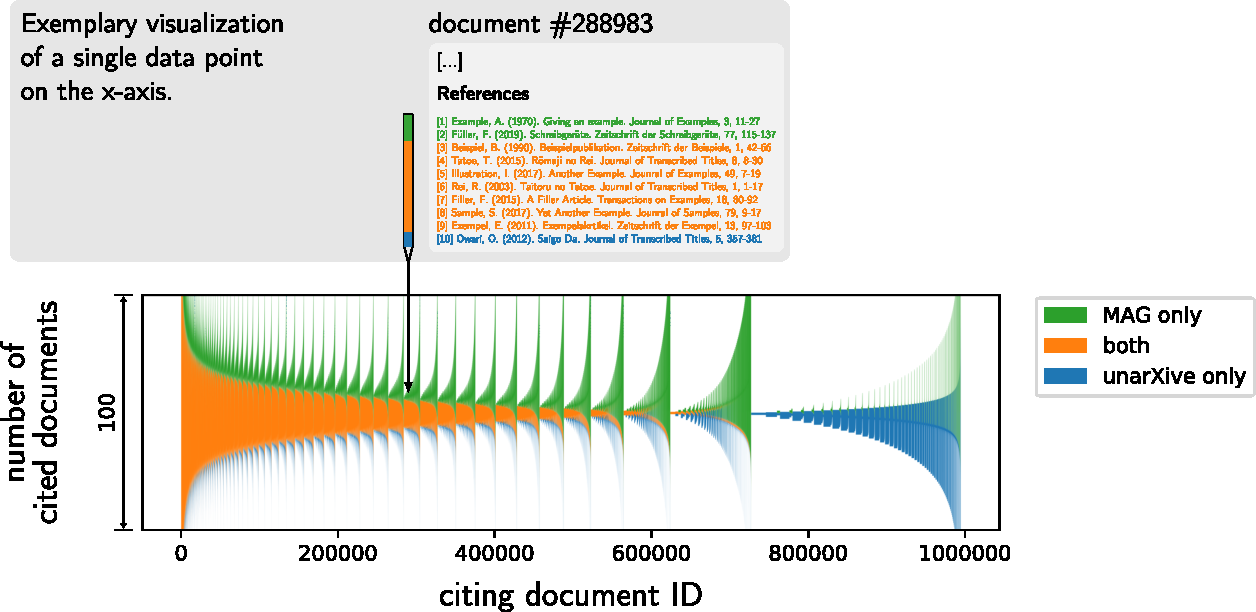
\includegraphics[width=\textwidth]{figures/corpus/Fig5.pdf}
  \caption[Composition of reference section coverage for all citing documents]{Composition of reference section coverage for all citing documents (cut off at 100 cited documents).}
  \label{fig:citcomp}
\end{figure}

\begin{figure}[tb]
  \centering
    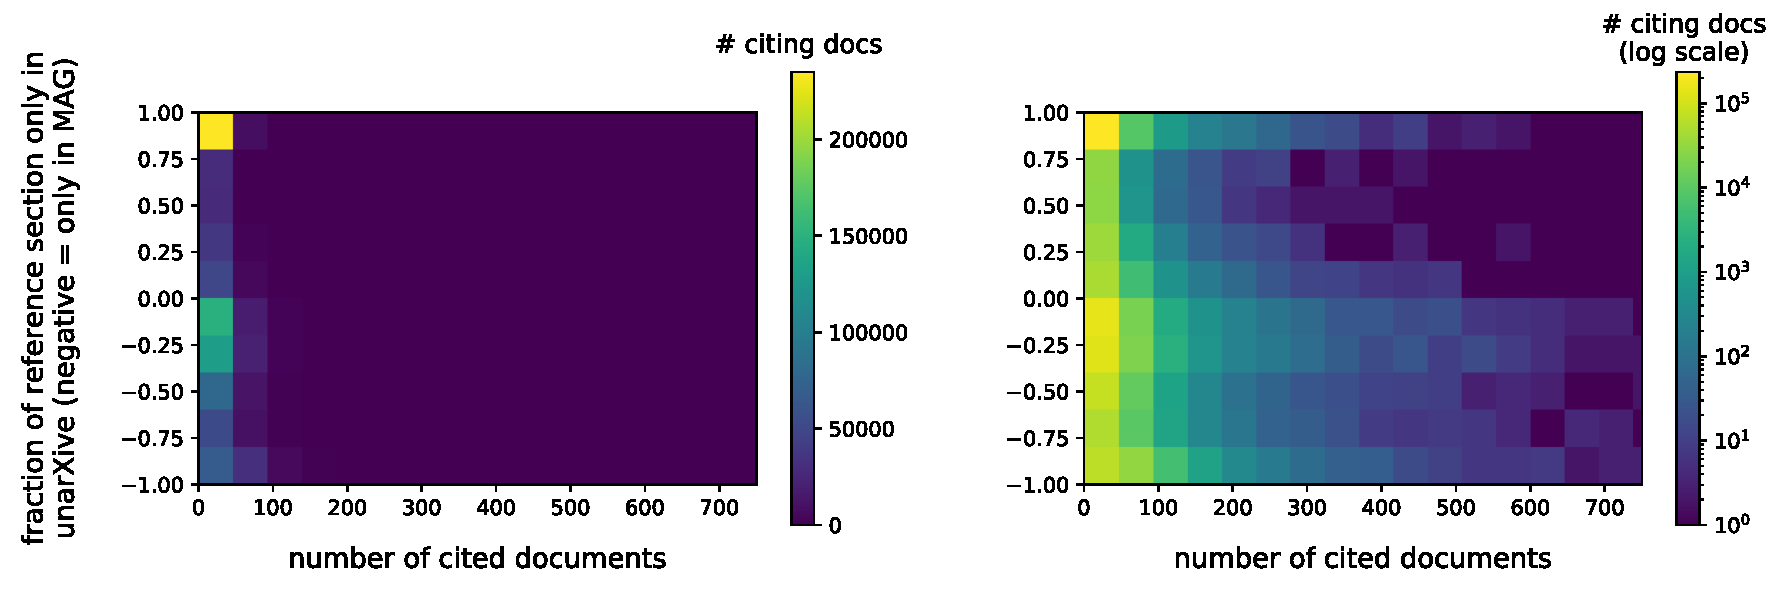
\includegraphics[width=\textwidth]{figures/corpus/Fig6.pdf}
  \caption[Distribution of citing documents in terms of reference section size and their coverage in unarXive and MAG]{Distribution of citing documents in terms of reference section size and their coverage in unarXive and MAG (cut off at 750 cited documents).}
  \label{fig:citcount2balance}
\end{figure}

Needless to say, additional references are only of value if they are valid. From both the citation links only found in unarXive, as well as those only found in the MAG, we therefore take a sample of 150 citing paper cited paper pairs and manually verify, if the former actually references the latter. This is done by inspecting the citing paper's PDF and checking the entries in the reference section against the cited paper's MAG record.\footnote{Further details can be found at \refurlinline{https://github.com/IllDepence/unarXive/tree/legacy_2020/doc/coverage_evaluation}{2023-11-06}.} On the unarXive side, we observe 4 invalid links, all of which are cases similar to those showcased in Table~\ref{tbl:mismatches}. On the MAG side, we observe 8 invalid links. Some of them seem to originate from the same challenges as the ones we face, e.g.\ similarly titled publications by same authors, leading to misidentified \emph{cited} papers. Other error sources are, for instance, an invalid source for a \emph{citing} paper being used and its reference section parsed (e.g.\ paper ID \texttt{1504647293}, where one of the PDF sources is the third author's Ph.D. thesis instead of the described paper). Given that the citation links exclusive to unarXive appear to be half as noisy as those exclusive to the MAG, we argue that the 5,918,128 links only found in unarXive could be useful for citation and paper based tasks using MAG data. This would especially be the case for the field of physics, as it makes up a significant portion of our data set.

\section{Analysis of Citation Flow and Citation Contexts}
\label{sec:analysis}

Because the documents in unarXive span multiple scientific disciplines, interdisciplinary analyses, such as the calculation of the flow of citations between disciplines, can be performed. Furthermore, the fact that documents are included as full-text and citation markers within the text are linked to their respective cited documents, makes varied and fine-grained study of citation contexts possible. To give further insight into our data set, we therefore conduct several such analyses in the following. Note that, for interdisciplinary investigations, disciplines other than physics, mathematics, and computer science are combined into \emph{other} for space and legibility reasons, as they are only represented by a small number of publications. On the citing documents' side, these span the fields of economics, electrical engineering and systems science, quantitative biology, quantitative finance, and statistics. Combined on the cited documents' side are chemistry, biology, engineering, materials science, economics, geology, psychology, medicine, business, geography, sociology, political science, philosophy, environmental science, and art.

\subsection{Citation Flow}

\begin{figure}
  \centering
    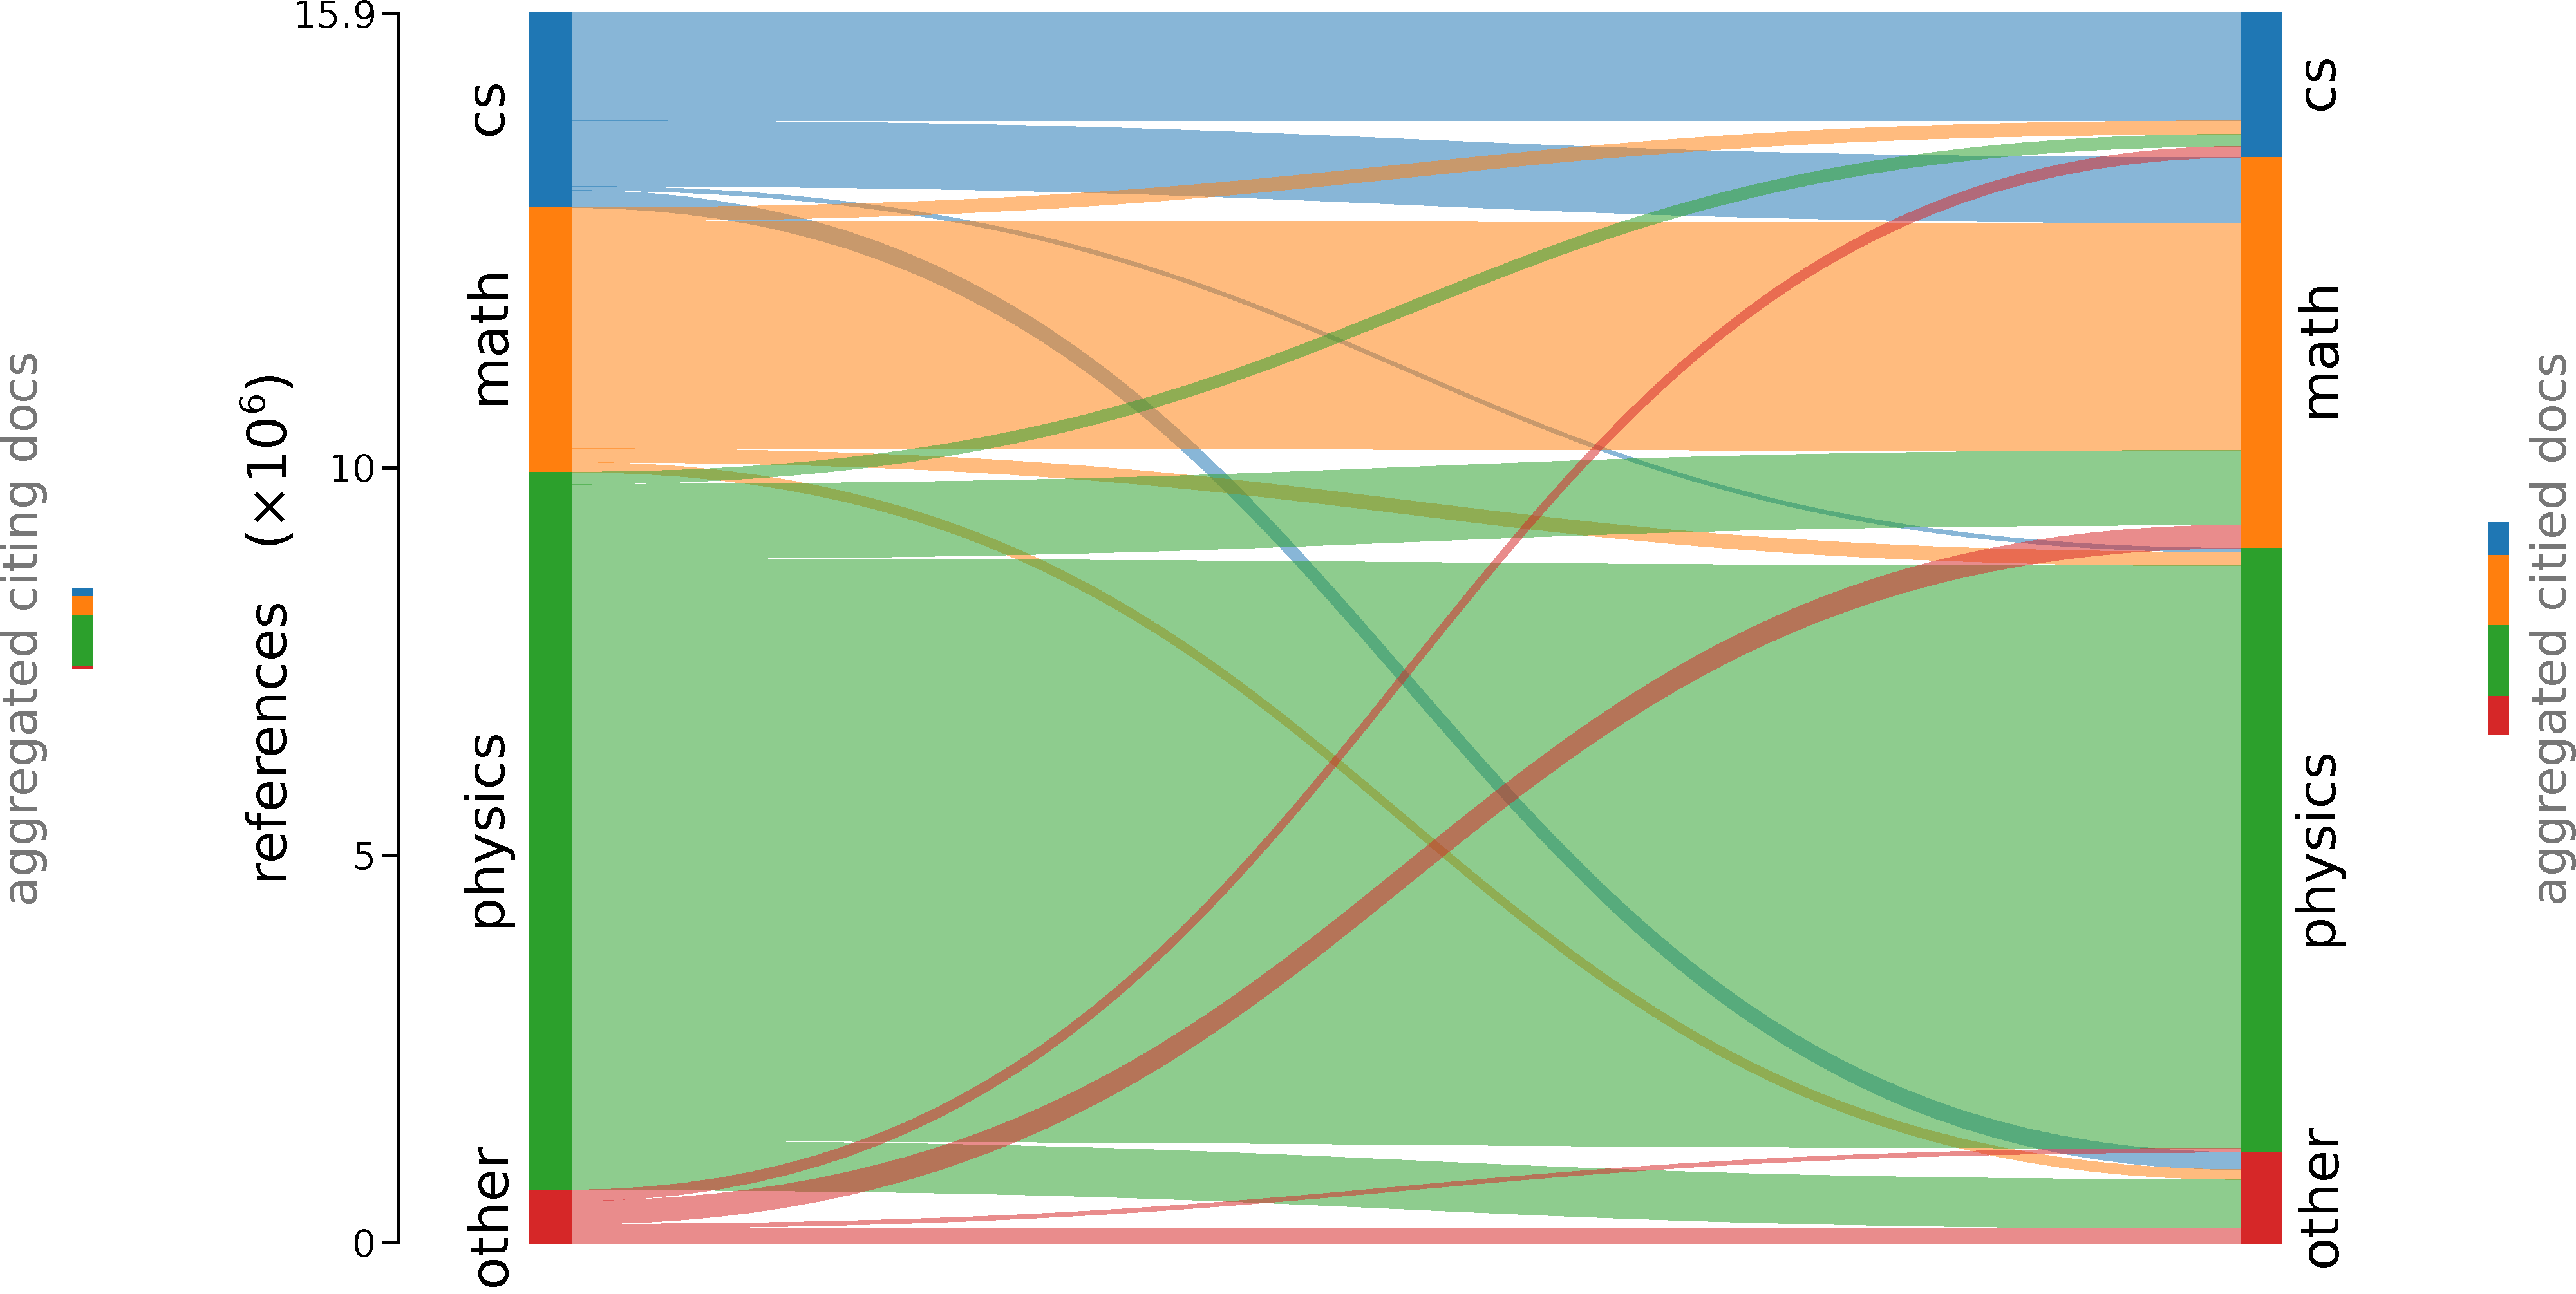
\includegraphics[width=0.97\textwidth]{figures/corpus/Fig7.pdf}
  \caption[Citation flow by discipline for 15.9 million references]{Citation flow by discipline for 15.9 million references (the number of citing and cited documents per discipline are plotted on the sides).}
  \label{fig:sankey}
\end{figure}

Figure~\ref{fig:sankey} depicts the flow of citations by discipline for all 15.9 million matched references. As one would expect, publications in each field are cited the most from within the field itself. Notable is, that the incoming citations in mathematics are the most varied (physics and computer science combined make up 35\% of the citations). As citation contexts are useful descriptive surrogates of the documents they refer to~\cite{Elkiss2008}, a composition as varied as mathematics in Figure~\ref{fig:sankey} bears the question whether a distinction by discipline could be worth considering, when using citation contexts as descriptions of cited documents. That is, computer scientists and physicists might refer to math papers in a different way than mathematicians do. Borders between disciplines are, however, not necessarily clear-cut, meaning that such a distinction might not be as straight forward as the color coding in Figure~\ref{fig:sankey} suggests.

\subsection{Availability of Citation Contexts}

\begin{figure}
  \centering
    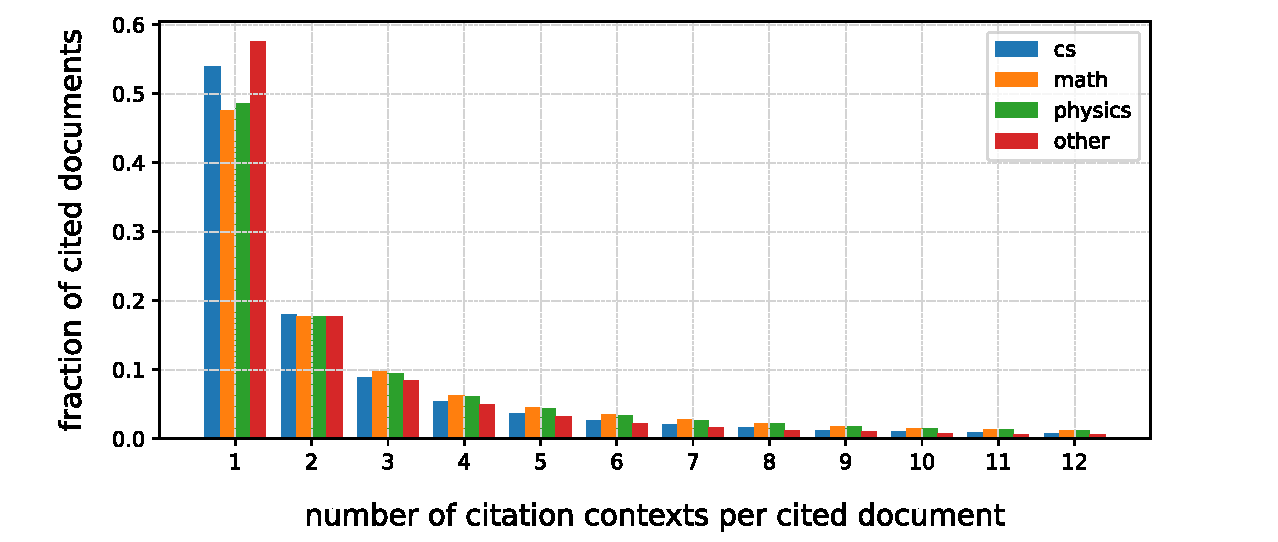
\includegraphics[width=\textwidth]{figures/corpus/Fig8.pdf}
  \caption[Normalized distribution of the number of citation contexts per cited document]{Normalized distribution of the number of citation contexts per cited document.}
  \label{fig:citcontextdist}
\end{figure}

Another aspect that becomes relevant, when using citation contexts to describe cited documents, is the number of citation contexts available per cited publication. Figure~\ref{fig:citcontextdist} shows, that the distribution of the number of citation contexts per cited document is similar across disciplines. In each discipline, around half of the cited documents are just mentioned once across all citing documents, 17.5\% exactly twice, and so on. The tail of the distribution drops a bit slower for physics and mathematics. The mean values of citation contexts per cited document are 9.5 (SD 50.3) in physics, 7.0 (SD 28.8) in mathematics, 5.1 (SD 31.1) in computer science and 3.5 (SD 11.0) for the combined other fields. This leads to two conclusions. First, it suggests that a representation relying solely on citation contexts may only be viable for a small fraction of publications. Second, the high dispersion in the number of available citation contexts shows that means might not be very informative when it comes to citation counts aggregated over specific sets of documents.

\subsection{Characteristics of Citation Contexts}
For our analysis of the contents of citation contexts, we focus on three aspects: whether or not citations are (1)~integral, (2)~syntactic and (3)~target section specific. These aspects were chosen, because they give particular insights into the citing behavior of researchers, as explained alongside the following definition of terms.

\subsubsection{``Integral'', ``Syntactic'' and ``Target Section Specific'' Citations}\label{sec:termdefs}
We first discuss the terms \emph{``integral''} and \emph{``syntactic''}, which are both established in existing literature. An integral citation is one, where the name of the cited document's author appears within the citing sentence \emph{and} has a grammatical role~\cite{Swales1990,Hyland1999} (e.g.\ ``Swales [73] has argued that ...''). Similarly, a citation is syntactic, if the \emph{citation marker} has a grammatical role within the citing sentence~\cite{Whidby2011,Abujbara2012} (e.g.\ ``According to [73] it is ...''). Integral citations are seen as an indication of emphasis towards the cited author (where the opposite direction would be towards the cited work)~\cite{Swales1990,Hyland1999}. Syntactic citations are of interest, when determining how a citation relates to different parts of the citing sentence~\cite{Whidby2011,Abujbara2012}. Both qualities are relevant when studying the role of citations~\cite{Faerber2019TPDL}.

\begin{table}
\centering
    \caption[Examples of citations and their categorization into integral/non-\allowbreak integral as well as syntactic/non-syntactic]{Examples of citations and their categorization into integral/non-\allowbreak integral as well as syntactic/non-syntactic (``\checkmark''=yes, ``$\times$''=no, ``?''=unclear).}
    \label{tab:integralsyntactic}
\begin{center}
    \begin{tabular}{llll|ll}
    \toprule
    \ & \rotatebox{90}{\cite{Swales1990}} & \rotatebox{90}{\cite{Hyland1999}} & \rotatebox{90}{\cite{Lamers2018}} & \rotatebox{90}{\cite{Whidby2011}} & \rotatebox{90}{\cite{Abujbara2012}} \\
    \ & \ & \ & \ & \ & \ \\
    Context excerpt (citation marker {\color{UniBlue}highlighted}) & \multicolumn{3}{c|}{\textbf{integral}} & \multicolumn{2}{l}{\textbf{syntactic}} \\
    \midrule
    ``Swales {\color{UniBlue}(1990)} has argued that ...''                 & \checkmark & \checkmark & \checkmark & $\times$ & ? \\
    ``{\color{UniBlue}Swales (1990)} has argued that ...''                 & \checkmark & \checkmark & $\times$ & \checkmark & \checkmark \\
    ``Swales {\color{UniBlue}[73]} has argued that ...''                   & \checkmark & \checkmark & \checkmark & $\times$ & $\times$ \\
    ``Swales has argued that ... {\color{UniBlue}[73]}''                   & \checkmark & \checkmark & \checkmark & $\times$ & $\times$ \\
    ``It has been argued {\color{UniBlue}(Swales, 1990)} that ...''        & $\times$ & $\times$ & $\times$ & $\times$ & $\times$ \\
    ``It has been argued {\color{UniBlue}[73]} that ...''                  & $\times$ & $\times$ & $\times$ & $\times$ & $\times$ \\
    ``According to {\color{UniBlue}(Swales, 1990)} it is ...''             & ? & ? & $\times$ & \checkmark & \checkmark \\
    ``According to {\color{UniBlue}[73]} it is ...''                       & $\times$ & $\times$ & $\times$ & \checkmark & \checkmark \\
    ``... has been shown (see {\color{UniBlue}(Swales, 1990)}).''          & $\times$ & $\times$ & $\times$ & \checkmark & $\times$ \\
    \bottomrule
    \end{tabular}
\end{center}
\end{table}

Table~\ref{tab:integralsyntactic} gives a more detailed account of both terms' use in literature. Note that~\cite{Lamers2018} provide a classification algorithm for integral and non-integral citations that slightly differs from Swales' original definition depending on the interpretation of a citation marker's scope, but also gives a clear classification in an edge case where Swales' definition is unclear. Furthermore note, that the two ways for distinguishing syntactic and non-syntactic citations found in literature are not identical. This is in part because the method given by~\cite{Abujbara2012} is kept rather simple. For the intents and purposes of our analysis we follow the definitions of Lamers et al.\ and Whidby et al.\ for \emph{``integral''} and \emph{``syntactic''} respectively.

\begin{table}
\centering
    \caption[Examples of target section specific citations]{Examples of target section specific citations.}
    \label{tab:secspec}
\begin{center}
    \begin{tabular}{l}
    \toprule
    Context excerpt ({\color{UniBlue}concerns citing document} / {\color{RandomRed}concerns cited document}) \\
    \midrule
    ``See [73], {\color{RandomRed}Section 3}.'' \\
    ``This improves {\color{RandomRed}Lemma 2} of [73], which is ...'' \\
    ``Due to this, the proof is now similar to that of {\color{RandomRed}Theorem 6.4} from [73].'' \\
    ``The copolymer version of {\color{UniBlue}Theorem 7} was derived in [73], {\color{RandomRed}Theorem 3.2}.''  \\
    ``{\color{UniBlue}Figure 1} is qualitatively similar to {\color{RandomRed}Figure 3} in [73].'' \\
    \bottomrule
    \end{tabular}
\end{center}
\end{table}

As a third aspect for analysis, we define \emph{``target section specific''} citations as those citations, where a specific section within the citation's target (i.e., the cited document) is referred to. Examples are given in Table~\ref{tab:secspec}. Target section specific citations are of interest for two reasons. First, in a similar fashion to integral citations, they are a particular form of citing behavior that might be used to infer characteristics of the relationship between citing author and cited document (e.g.\ a focus on the document rather than authors, or in-depth engagement or familiarity with the cited document's contents). Second, when using citation contexts as descriptions of cited documents, such as in citation context-based document summarization, target section specific citations might benefit from special handling, as their contexts only describe a (sometimes very narrow) part of the cited document.

In the following we will analyze all three aspects (integral, syntactic, target section specific) with respect to the different scientific disciplines covered by our data set.

\subsubsection{Manual Analysis of Citation Contexts}

\begin{table}[tb]
\centering
  \caption[Per discipline number of citations labeled integral, syntactic, imultaneously integral and syntactic, target section specific]{Per discipline number of citations labeled (1)~integral, (2)~syntactic, (3)~simultaneously integral and syntactic, (4)~target section specific (sample size = 300).}
  \label{tbl:integralsyntacticsecspec}
\begin{small}
\begin{tabular}{lrrrr}
\toprule
   Discipline & Integral & Syntactic & Integral+Syntactic & Target Section Specific \\
   \midrule
   Computer Science & 23 & 88 & 1 & 5 \\
   Mathematics & 48 & 200 & 13 & 17 \\
   Physics & 12 & 80 & 2 & 4 \\
   Other & 14 & 113 & 1 & 7 \\
  \bottomrule
\end{tabular}
\end{small}
\end{table}

For each of the disciplines computer science, mathematics, physics, and other, we take a random sample of 300 citation contexts and manually label them with respect to being integral, syntactic, and target section specific. The result of this analysis is shown in Table~\ref{tbl:integralsyntacticsecspec}. Each of the assigned labels is most prevalent in mathematics papers, which is furthermore true for the co-occurrence of the labels integral and syntactic. Mathematics is also the only discipline, in which citations are more likely to be syntactic than not. The difference in frequency of integral and syntactic citations might be due to variations in writing culture between the different disciplines. We think that the comparatively high frequency of target section specific citations in mathematics could be due to the fact, that in mathematics intermediate results like corollaries and lemmata are immediately reusable in related work. We further investigate target section specific citations in the following section.

\subsubsection{Automated Analysis of Target Section Specific Citations}\label{sec:specrevautoeval}
Sentences including a target section specific citation often follow distinct and predictable patterns. For example, a capitalized noun (e.g.\ \emph{``Corrolary''}, \emph{``Lemma''}, \emph{``Theorem''}) is followed by a number and a preposition (e.g.\ \emph{``in''},  \emph{``of''}), and then followed by the citation marker (e.g.\ \emph{``Corrolary 3 in [73]''}). Another pattern is the citation marker followed by a capitalized noun and a number (e.g.\ \emph{``[73] Lemma 7''}). This lexical regularity allows us to identify target section specific citations in an automated fashion. Specifically, we search the entirety of our 29 M citation contexts for word sequences, that match either of the part of speech tag patterns \texttt{NNP~CD~IN~<citation~marker>} and \texttt{<citation~marker>~NNP~CD}. Doing this, we find 365,299 matches (1.25\% of all contexts). This is less than the 2.31\% one would expect due to the manual analysis\footnote{Because disciplines are not equally represented in the data set, the expected value is not simply the average of values in Table~\ref{tbl:integralsyntacticsecspec} ($\frac{5+17+4+7}{4}\times 300^{-1}=0.0275$), but a weighted average $(5\times w_\text{cs}+17\times w_\text{math}+4\times w_\text{phys}+7\times w_\text{other})\times 300^{-1}$, with $\sum w_{\langle\text{discipline}\rangle}=1$. This gives a value of $\approx 0.0231$.} and suggests, that above two patterns are not exhaustive. Nevertheless, we can use the identified contexts to further analyze them with respect to their distribution of disciplines.

% normalization factors:
%
% 15,954,664/...
%
% citing:              cited:
% math: 3,426,117      5,062,033
% cs:   2,526,656      1,876,401
% phys: 9,300,576      7,827,072
% other:  701,315      1,189,158
%
% pairs:
%
%    phys→phys 7,543,495
%    phys→math 967,263
%    phys→cs 157,338
%    math→phys 177,502
%    math→math 2,947,360
%    math→cs 173,168
%    cs→phys 51,942
%    cs→math 847,932
%    cs→cs 1,402,081

\begin{table}[tb]
\centering
  \caption[Occurrence of target section specific citations by discipline]{Occurrence of target section specific citations by discipline (pairs annotated as follows, \textsuperscript{\textdagger}:~Mathematics citing document, \textsuperscript{\textdaggerdbl}:~Mathematics cited document, \underline{X$\rightarrow$X}:~Citing and cited document are from the same discipline).}
  \label{tbl:secref}
\begin{small}
\begin{tabular}{llrrr}
\toprule
   \ & Discipline & Count & Normalization factor & Normalized ratio (\%) \\ % "normalized count"
   \midrule
   \textbf{Citing} & Mathematics & 298,009 & 4.66 & 8.70 \\ % 1,388,722
   \ & CS & 9,123 & 6.31 & 0.36 \\ % 57,608
   \ & Physics & 30,593 & 1.72 & 0.33 \\ % 52,480
   \midrule
   \textbf{Cited} & Mathematics & 313,651 & 3.15 & 6.20 \\ % 988,574
   \ & CS & 12,179 & 8.50 & 0.65 \\ % 103,556
   \ & Physics & 31,087 & 2.04 & 0.40 \\ % 63,368
   \midrule
   \textbf{Pairs} & \underline{Math\textsuperscript{\textdagger}$\rightarrow$Math\textsuperscript{\textdaggerdbl}} & 200,859 & 5.41 & 6.81 \\ % 1,087,290
   \ & Math\textsuperscript{\textdagger}$\rightarrow$CS & 5,134 & 92.13 & 2.96 \\ % 472,995
   \ & Math\textsuperscript{\textdagger}$\rightarrow$Phys & 3,114 & 89.88 & 1.75 \\ % 279,900
   \ & CS$\rightarrow$Math\textsuperscript{\textdaggerdbl} & 3,456 & 18.82 & 0.41 \\ % 65,028
   \ & Phys$\rightarrow$Math\textsuperscript{\textdaggerdbl} & 3,859 & 16.49 & 0.40 \\ % 63,653
   \ & \underline{CS$\rightarrow$CS} & 2,500 & 11.38 & 0.18 \\ % 28,448
   \ & \underline{Phys$\rightarrow$Phys} & 10,374 & 2.12 & 0.14 \\ % 21,941
   \ & CS$\rightarrow$Phys & 50 & 307.16 & 0.10 \\ % 15,358
   \ & Phys$\rightarrow$CS & 137 & 101.40 & 0.09  \\ % 13,892
  \bottomrule
\end{tabular}
\end{small}
\end{table}

Table~\ref{tbl:secref} shows the results of this subsequent analysis. Because our data set does not contain equal numbers of citations from each discipline (see Figure~\ref{fig:sankey}), we normalize the absolute numbers of pattern occurrences. Rows are then sorted by normalized ratio in decreasing order. Looking at the citing documents (those in which the pattern was found), we see a similar picture to the one in our manual analysis (shown in Table~\ref{tbl:integralsyntacticsecspec}). Namely, mathematics with the highest count of target section specific citations by far, and a similar count for computer science and physics, where the latter is slightly lower. Counting by the cited documents (the document in which a specific part is being referenced), the differences decrease a little bit, but mathematics still occurs most frequently by far.

An interesting pattern emerges, when taking an even more detailed look and breaking these citations down by the disciplines on \emph{both} sides of the citation relation. We then can observe the following.
\begin{itemize}
 \item The most determining factor for target section specific citations seems to be, that a mathematician is writing the document.\textsuperscript{\textdagger} As with integral and syntactic citations, the writing culture of the field might play a role here.
 \item The second most determining factor then appears to be, that a mathematical paper is being cited.\textsuperscript{\textdaggerdbl}. Mathematics documents might lend themselves to being cited in this way.
 \item The third most determining factor is an \underline{intra-discipline citation} (i.e., the citing document is from that same discipline as the cited). This supports the interpretation of target section specific citations as a sign of familiarity with what is being cited (see Section~\ref{sec:termdefs}).
\end{itemize}

Math$\rightarrow$Math pairs, where all three of the above factors come into play simultaneously, consequentially show the highest occurrence of target section specific citations by far.

To summarize the results of our analysis of citation flow and citation contexts, we note the following points.

\begin{itemize}
    \item Publications in mathematics are cited from ``outside the field'' (e.g.\ by computer science or physics papers) to a comparatively high degree. Distinguishing citation contexts referring to mathematics publications by discipline might therefore be beneficial in certain applications (e.g.\ citation-based automated survey generation).
    \item For most publications, only one or a few citation contexts are available.
    \item Integral citations appear to be about twice as common in computer science as they are in physics, and again twice as common in mathematics as they are in computer science. Going with Swale's interpretation of the phenomenon, this would mean the focus put on authors in mathematics is higher than in computer science, and higher in computer science than in physics.
    \item In mathematics, syntactic citations seem to be more common that non-syntactic citations. This is beneficial for reference scope identification~\cite{Abujbara2012} and any sophisticated approaches based on citation contexts (like context-aware citation recommendation), as citation markers in syntactic citations stand in a grammatical relation to their surrounding words.
    \item We define target section specific citations as those citations, where a specific section within the cited document is referred to. This type of citation is the most common in mathematics (comparing mathematics, computer science and physics). Through a subsequent analysis of 365k target section specific citations, we find that they are more common in intra-discipline citations than in inter-discipline citations. This supports our assumption that they are an indicator for familiarity with the cited document.
\end{itemize}

Our work regarding the five aspects outlined in the beginning, namely \emph{size}, \emph{cleanliness}, \emph{global citation annotations}, \emph{data set interlinkage}, \emph{cross-domain coverage}, enabled above results. Without sufficient size, our results would be less informative. If our documents contained too much noise, the quality of reference resolution would have deteriorated. Global citation annotations, especially because of their word level precision, make fine-grained lexical analyses of citation contexts like the one in Section~\ref{sec:specrevautoeval} possible. Without interlinking our data set to the MAG, available metadata would have been scarce. While we mainly focused on the scientific discipline information in the MAG, there is much more (authors, venues, etc.) that can be worked with in future analyses. Lastly, if our data set would have only covered a single scientific discipline, an analysis of citation flow, as well as interdisciplinary comparisons of citation context criteria would not have been possible.

\section{Conclusion}
\label{sec:conclusion}

Evaluating and applying approaches to research paper-based and citation-based tasks typically requires large, high-quality, citation-annotated, interlinked data sets. In this chapter, we proposed a new data set with over one million papers' full-text, 29.2 million annotated citations, and 29.2 million extracted citation contexts (of three sentences each), ready to be used by researchers and practitioners.
We provide the data set and the implementation for creating the data set from arXiv source files online for further usage.

% For the future, we plan to use the data set for a variety of tasks. Among others, we will develop a citation recommendation system based on all arXiv papers. Furthermore, we plan to perform additional analyses on citations and citation contexts across scientific disciplines, and to use the differences in citing behavior for enhanced citation recommendation.

\section*{Author Contributions}  % see https://casrai.org/credit/
Tarek Saier: Conceptualization, Data curation, Formal analysis, Investigation, Methodology, Software, Visualization, Writing -- original draft, Writing -- review \& editing. Michael F{\"a}rber: Supervision, Writing -- review \& editing.

\section{Result Assessment}
\label{sec:corpus-assessment}

The work in this chapter primarily addresses the following research task.

\begin{rtlist}
    \item \textit{Base Methodology} - establish a base methodology for generating a large-scale, high-quality scholarly data set, that is on par with or improving upon existing data sets.
\end{rtlist}

The presented methodology and resulting corpus \emph{unarXive} are on par or improve upon the identified related work both in terms of scale and quality. Regarding scale, \emph{unarXive} (1\,M documents) is among the top three alongside CiteSeerX (1\,M) and the PMC OAS (2.3\,M). Considering quality, using \LaTeX{} source files ensures less noisy full-text compared to data sets generated from PDFs, and the established citation network links proved to be highly accurate in a manual evaluation. Accordingly, we deem \rtmark{1} successfully achieved.

The work presented in this chapter furthermore makes contributions to the following research task.

\begin{rtlist}
    \item[\rtmark{2}:] \textit{Citation Network Completeness} - develop a method to link literature references, that is able to link more references than are linked in existing data sets, while not compromising on link correctness or processing efficiency.
\end{rtlist}

% \cite{Faerber2018LREC}
% @Sec 4
% All papers reference 277,227 unique papers using
% 2,448,826 citation markers in total (i.e., on average 27.1
% citation markers per citing paper). Of these references,
% 962,084 could be found on DBLP and we could assign
% them a DBLP URL.
% 962,084/2,448,826 = 0,3928

The reference linking method developed for \emph{unarXive} is able to link 42.6\% of references successfully to the MAG. While no data set with which a direct comparison would be possible existed at the time of publication, the number compares favorably to arXiv CS achieving 39.3\%\footnote{962,084 out of 2,448,826 references are reported to be successfully linked in the arXiv CS paper~\cite{Faerber2018LREC}.}, and also can be considered an improvement over the PMC OAS with no consistent citation network as well as CiteSeerX with no assessment resented for its citation network. Accordingly, we deem this a significant contribution to \rtmark{2}.

In terms of the overarching research goal of enabling higher-quality scholarly data (see Table~\ref{tab:scholdataquali} in Chapter~\ref{chp:foundations}), the work presented in this chapter makes the following contributions.

\begin{infobox-progress}
      \textbf{Scholarly Data Quality Contributions - \cite{Saier2020}}\vspace{0.5em}

      \begin{tabular}{lp{10.9cm}}
        \toprule
        Crit. & Contribution \\
        \midrule
        $\mathbf{Rel_{CN}}$ & First data set based on all of arXiv with a citation network \\
        $\mathbf{Acc_{CN}}$ & $>96$\% accurate reference matching method (SOTA) \\
        $\mathbf{Acc_{SDR}}$ & Low-noise text extraction by using \LaTeX{} as data source \\
        $\mathbf{Tim_{C/S}}$ & Publications included up until end of the most recent full year \\
        $\mathbf{Coy_{CN}}$ & MAG and arXiv IDs included; DOIs linked through MAG records \\
        $\mathbf{Cos_{CN}}$ & 42.6\% reference matching success rate (SOTA) \\
        $\mathbf{Cos_{SDR}}$ & Full-text of documents included \\
        \bottomrule
      \end{tabular}
\end{infobox-progress}

$\mathbf{Rel_{CN}}$ We provide the first data set based on all of arXiv with a citation network. Previous data sets only cover part of arXiv~\cite{Faerber2018LREC}, or do not include a citation network~\cite{arXMLiv}. By covering all of arXiv, the data is of high relevance for use cases focussing on physics, mathematics, or computer science. % Could additionally mention that, because maths is cited a lot in physics and CS, the data also includes data on relevant closely related documents
Because documents submitted to arXiv undergo a moderation process\refurl{https://info.arxiv.org/help/moderation/index.html}{2024-02-03} in which they are assigned to a topic according to the arXiv taxonomy,\refurl{https://arxiv.org/category_taxonomy}{2024-02-03} a fine-granular and reliable determination of relevance to a subject of study is possible. While documents on arXiv are by designation preprints, most of them are self-archived author copies which later appear in peer-reviewed venues---between 75\% and 80\% averaged over all disciplines, measured on all papers from 2008 to 2017~\cite{Lin2020}, and at 90.1\% in computer science measured on a sample of 18 thousand papers from 2022~\cite{Bagchi2024} .

$\mathbf{Acc_{CN}}$ Our reference linking method is evaluated at an accuracy of $>96$\%. By comparison, CiteSeerX~\cite{Wu2015,Wu2016,Patel2021} provides no assessment of their citation network accuracy, and S2ORC~\cite{Lo2020} (published shortly after unarXive) only achieves a matching accuracy of 92\% on arXiv papers. Our work accordingly achieves state-of-the-art citation network accuracy.

$\mathbf{Acc_{SDR}}$ We create document representations not from PDF files but from papers' \LaTeX{} sources. Text extraction from \LaTeX{} has been used to generate ground truths for the evaluation of from PDF documents~\cite{Bast2017}. Accordingly, we argue that our method constitutes an improvement for the accuracy of document representations compared to PDF based approaches.

$\mathbf{Tim_{C/S}}$ We apply our method for generating scholarly data on all documents on arXiv until end of the most recent full year. Accordingly, the resulting corpus contains more recent documents than data sets released earlier.

$\mathbf{Coy_{CN}}$ We provide MAG IDs and arXiv IDs for the documents in our corpus. Furthermore, DOIs are available through the liked MAG paper records. Enabling the use of three different types of unique identifiers makes our data a versatile target for comparing and combining it with other data. Other data sets of comparable size only provide their own identifiers (CiteSeerX) or only feature a heterogeneous set of identifiers (PMC OAS).

$\mathbf{Cos_{CN}}$ We are able to successfully link 42.6\% of all reference in our data. This makes our citation network more complete than that of comparable existing data sets. Other approaches do not provide an assessment of their citation network completeness (CiteSeerX), or only achieve a lower percentage (arXiv CS achieving 39.3\%).

$\mathbf{Cos_{SDR}}$ For all documents in our data set we provide their full-text content. This means our document representations are more complete that those in metadata sets like the MAG, and on par with other data sets providing full-text such as CiteSeerX and PMC OAS. \\

% quantification / good enough

% $\mathbf{Rel_{CN}}$ Improved relevance, by providing extensive coverage of physics, mathematics, and computer science papers \\
% numbers from arXiv? / mby 80/20 rule ppr?

% $\mathbf{Acc_{CN}}$ Improved citation network accuracy, by introducing $>96$\% accurate reference matching method \\
% ✓ / ?

% $\mathbf{Acc_{SDR}}$ Improved document representation accuracy, due to low noise through using \LaTeX{} as the data source \\
% Bast ppr? / ?

% $\mathbf{Tim_{C/S}}$ Improved coverage, by including publications up until the end of the most recent full year \\
%  ✓ / ? depends on use case lel

% $\mathbf{Coy_{CN}}$ Improved comparability, by providing MAG and arXiv IDs, as well as DOIs through the linked MAG records \\
% #of records IDd? / 

% $\mathbf{Cos_{CN}}$ Improved citation network completeness, by achieving 42.6\% reference matching success rate (SOTA) \\
% ✓ / probably not

% $\mathbf{Cos_{SDR}}$ Improved document representation completeness, by providing full-text \\
% 


% = @ topic fit
% - arXiv moderation process \refurl{https://info.arxiv.org/help/moderation/index.html}{2024-02-03}
%   - "guaranteed" topic fit
%   - topic fit given in metadata according to taxonomy -> better than venue/journal b/c often not that granular
%
% = @ how much of arXiv later published ("precision")
% - \cite{Lariviere2014}
%   - 474,011 out of the 744,583 arXiv e-prints (63.7%) were matched with a WoS-indexed journal article, note, or review (2014)
% - \cite{Lin2020}
%   - ~75-80% overall (data from 2008-2017)
%   - 77.1% of CS,
% - \cite{Bagchi2024}
%   - 90.1% of CS papers put on arXiv in 2022 (from 48.6% in 2013) (18,113 article data set)
%
% = @ how much of all publications on arXive ("recall")
% - \cite{Sutton2017}
%   - arXiv 23% CS coverage in 2017 (from 1% in 2007) (82,427 paper data set)
%   - in theoretical CS and ML, over 60% of top conf pprs on arXiv

\chapter{Reference Coverage and Granularity}
\label{chp:covgran}

This chapter is based on the following publications.
\begin{infobox-pub}
\fullcite{Saier2022ULITE}
\end{infobox-pub}

\begin{infobox-pub}
\fullcite{Saier2023unarXive}
\end{infobox-pub}

\section{Overview}
In this chapter, we introduce improvements for our corpus creation methodology in two areas.
First, we present in Section~\ref{sec:covgran-blocking} a blocking and matching method applied on the set of references in a corpus. With this matched references as well as bibliographic couplings can significantly be increased. % Furthermore, it removes the reliance of a ...
Second, we present in Section~\ref{sec:covgran-ux22} an improved conversion method for \LaTeX\ source files, and with it an update of the \emph{unarXive} corpus. The improved corpus creation method enables fine-granularly structured document representations, and achieves a new state-of-the-art reference matching success rate.\footnote{After the publication of our initial corpus creation methodology in \cite{Saier2020} (see Chapter~\ref{chp:corpus}), the now widely used corpus S2ORC~\cite{Lo2020} adapted our document conversion methodology for the \LaTeX\ subset of their data set. While they do not achieve a reference matching success rate as high as ours, they made advances regarding the structured document representation. With the work presented in this chapter, we follow and improve upon their example, establishing a fine-granular structured document representation for the \emph{unarXive} corpus.}

In terms of the overarching research goal of enabling higher-quality scholarly data (see Table~\ref{tab:scholdataquali} in Chapter~\ref{chp:foundations}), the work presented in this chapter makes the following contributions.

\begin{infobox-progress}
      \textbf{Scholarly Data Quality Contributions - \cite{Saier2022ULITE,Saier2023unarXive}}\vspace{0.5em}

      \begin{tabular}{cp{11.3cm}}
        \toprule
        Crit. & Explanation \\
        \midrule
        \textbf{C2} & Improved relevance, by adding mathematical notation as well as figure and table captions to the document representation \\
        \textbf{C5} & Improved coverage, by including publications up until the end of the most recent full year \\
        \textbf{C6} & Improved comparability, by providing OpenAlex and arXiv IDs, as well as DOIs through the linked OpenAlex records \\
        \textbf{C8} & Improved citation network completeness, by introducing blocking and matching procedure \\
        \textbf{C9} & Improved document representation completeness, by providing full-text with mathematical notation preserved as \LaTeX \\
        \bottomrule
      \end{tabular}
\end{infobox-progress}

% \begin{abstract}
% Analyses and applications based on bibliographic references are of ever increasing importance. However, reference linking methods described in the literature are only able to link around half of the references in papers. To improve the quality of reference linking in large scholarly data sets, we propose a blocking-based reference linking approach that utilizes a rich set of reference fields (title, author, journal, year, etc.) and is independent of a target collection of paper records to be linked to. We evaluate our approach on a corpus of 300,000 references. Relative to the original data, we achieve a 90\% increase in papers linked through references, a five-fold increase in bibliographic coupling, and a nine-fold increase in in-text citations covered. The newly established links are of high quality (85\% $\text{F}_1$ score). We conclude that our proposed approach demonstrates a way towards better quality scholarly data.
% \end{abstract}

% \section{A Blocking-Based Approach to Enhance Large-Scale Reference Linking}
\section{Reference Linking by Inter-Reference Blocking}\label{sec:covgran-blocking}

\subsection{Introduction}
% % Motivation
Scholarly data is becoming increasingly important and with it its quality and coverage. Connections between publications in the form of literature references are of particular importance, as they are used as a basis for various analyses, decision making, and applications. Some examples are research output quantification~\cite{Hirsch2005}, trend detection~\cite{Chen2006}, summarization~\cite{Elkiss2008}, and recommendation~\cite{Ma2020,Faerber202x}.

% Problem
%However, in current data sets providing interlinked publications, only around half of the references contained in the original papers are linked\footnote{We use ``link[ing/ed] references'' w.r.t. to connections to cited papers rather than in-text citation markers.} to the cited publications~\cite{Lo2020,Saier2020}. This lack in coverage is especially affecting references to non-English publications~\cite{Saier2021}, which are in general underrepresented in scholarly data~\cite{Vera-Baceta2019,Liu2019,Moed2018,Moskaleva2019} along with publications in the humanities~\cite{Colavizza2019,Kellsey2004}.
However, reference linking methods\footnote{In the following, we use ``link[ing/ed] references'' to refer to connections to cited papers rather than in-text citation markers.} described in the literature are only able to link around half of the references contained in the original papers to the cited publications~\cite{Lo2020,Saier2020}. This lack in coverage is especially affecting references to non-English publications~\cite{Saier2021}, which are in general underrepresented in scholarly data~\cite{Vera-Baceta2019,Liu2019,Moed2018,Moskaleva2019} along with publications in the humanities~\cite{Colavizza2019,Kellsey2004}.

We see the reason for this lack in linked references in two key shortcomings of current methods.
First, references are linked using simple string similarity measures that are often relying \emph{only} on publications' title and author information (which is not always contained in references; see Figure~\ref{fig:hardmatch}). %Note: maybe add sth. along the lines of “relying on title (and mby authors) is deemed sufficient”
Second, references are exclusively linked to a target collection of paper records---usually a large metadata set like DBLP\refurl{https://dblp.org/}{2023-11-10} or OpenAlex,\refurl{https://openalex.org/}{2023-11-10} or a set of IDs like DOIs or PMIDs. This means references to literature which is not contained in the target collection, as well as to non-source items~\cite{Chi2014}, cannot be linked (see ``?'' markers in Figure~\ref{fig:approach}).

\begin{figure}[tb]
  \centering
  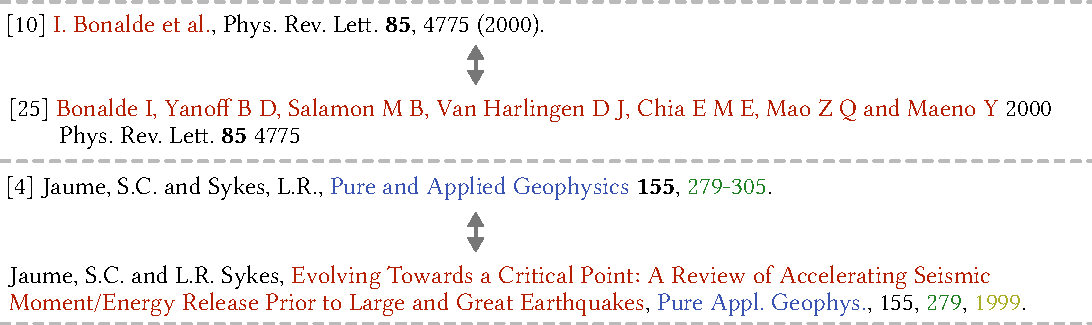
\includegraphics[width=\linewidth]{figures/ref_covgran/hardmatch_examples.pdf}
  \caption[Examples of challenging reference pairs from our evaluation that where successfully matched]{Examples of challenging reference pairs from our evaluation that where successfully matched. \textbf{Top:} references from \texttt{arXiv:cond-mat/0503317} (no title, first author only) and \texttt{arXiv:cond-mat/0104493} (no title, all authors). \textbf{Bottom:} references from \texttt{arXiv:cond-mat/0104341} (no title, full venue, page rage, no year) and \texttt{arXiv:physics/0504218} (with title, venue abbreviation, start page only, with year).}
  \label{fig:hardmatch}
\end{figure}

\begin{figure}[tb]
  \centering
  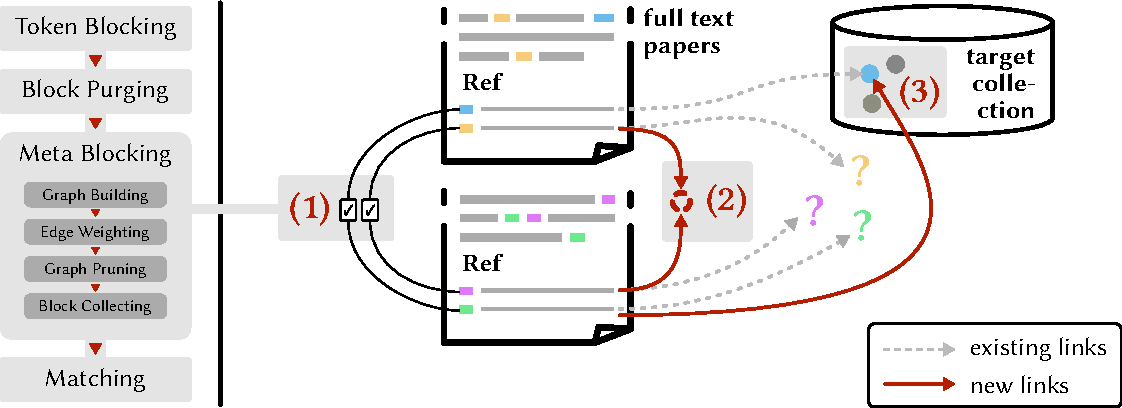
\includegraphics[width=\linewidth]{figures/ref_covgran/approach_withblocking_10pvar.pdf}
  \caption[Schematic depiction of the use case]{Schematic depiction of the use case. A corpus of full-text papers, where some references are already linked to a target collection (blue), and some are not (orange, pink, green). At \textbf{(1)} we apply our blocking and matching approach to identify all references that point to the same publication. In doing so, we establish new links in the form of \textbf{(2)} bibliographic coupling and \textbf{(3)} links to the target collection.}
  \label{fig:approach}
\end{figure}

%ER related work
Linking references can be seen as a task of entity resolution (ER)~\cite{Christophides2015ERdef}, which is concerned with identifying entities referring to the same object within or between large data sets. Because the task requires a one-to-one comparison between each of the involved entities, it is inherently of quadratic complexity. To make approaches scalable, entities are assigned into groups of likely matching candidates prior to comparison, a technique called blocking~\cite{Papadakis2020survey}.
While blocking-based approaches are used in the domain of scholarly data to, for example, identify duplicate paper records~\cite{Simonini2016blast,Sefid2019,Lo2020} (where information such as abstracts are used) and authors~\cite{FaerberLin2022}, they are not utilized for bibliographic references.

% Our solution
We therefore address both of the aforementioned problems with current reference linking approaches, (1)~the use of simple matching methods based on title and authors, as well as (2)~the reliance on a target collection of paper records, by proposing (1)~the use of a blocking and matching process utilizing seven reference fields (title, author, journal, year, etc.) that (2)~operates \emph{within} the set of bibliographic references of a corpus, and is thereby \emph{independent} of a target collection of papers (see marker ``(1)'' in Figure~\ref{fig:approach}).

We showcase the feasibility and benefits of our approach, implementing a pre-processing, blocking, and matching pipeline and evaluating it on a corpus containing 300,000 references.
We show that relative to the original data, our approach gives us a \textbf{90\% increase} in papers linked to the target collection, a \textbf{five-fold increase} in bibliographically coupled~\cite{Boyack2010} papers (see marker ``(2)'' in Figure~\ref{fig:approach}), and a \textbf{nine-fold increase} in in-text citation markers covered.\footnote{With the ``coverage'' of in-text citation markers we refer to markers associated with linked references, relative to markers belonging to unlinked references.} The new links are furthermore of high quality (85\% $\text{F}_1$ score). This paves the way towards higher quality scholarly data, especially regarding the coverage of so far underrepresented literature and non-source items.

In summary, we make the following contributions.

\begin{itemize}
    \item We propose a blocking-based approach for matching bibliographic references that is independent of a target collection of paper records.
    \item We perform a large-scale evaluation showing that our approach results in a manifold increase in high quality reference links.
    \item We make our data and code publicly available.\refurl{https://github.com/IllDepence/ulite2022}{2023-11-10}
\end{itemize}

\subsection{Related Work}
Blocking-based approaches have been used in the domain of scholarly data, though to the best of our knowledge not for bibliographic references. We therefore report on (1) exemplary uses of blocking in the scholarly domain for entities other than references, and (2) approaches to linking bibliographic references using methods other than blocking.

Simonini et al.~\cite{Simonini2016blast} develop BLAST (Blocking with Loosely-Aware Schema Techniques) which adapts Locality-Sensitive Hashing. Among data sets from other domains, they also evaluate their approach for the task of linking 2,600 DBLP paper records to the ACM\refurl{https://dl.acm.org/}{2023-11-10} and Google Scholar.\refurl{https://scholar.google.com/}{2023-11-10} 
Sefid~\cite{Sefid2019} proposes several models to match paper records utilizing the papers' title, header, and citation information. The models are evaluated in three scenarios matching 1,000 paper records from CiteSeer$^x$~\cite{CiteSeerX2019} to IEEE, DBLP, and Web of Science.
Lastly, Färber et al.~\cite{FaerberLin2022} detect duplicates among 243 million author records in the Microsoft Academic Knowledge Graph~\cite{MAKG} and evaluate their approach using ORCiD IDs.

%                        GROBID | LaTeX
% Bibliography entries   27.6M  | 21.9M*
% Linked bib. entries    19.3M  |  6.8M*
%
% *The lower number of linked bibliography entries in latex parses is due to large numbers of papers (mostly in the field of physics) for which the bibliography entries are formatted without paper titles. Our linking algorithm strongly depends on titles and fails to link these entries.
Lo et al.~\cite{Lo2020} introduced the data set S2ORC, which contains 9.6 million open access papers and has recently seen extensive use in area of scholarly document processing. The authors link references to papers within their data set using a heuristic similarity measure based on n-grams and the Jaccard similarity, which only uses the paper title. Using this method, 26 million out of 50 million references  (52\%) are successfully linked. The authors report that the low number is \textit{``due to large numbers of papers (mostly in the field of physics) for which the bibliography entries are formatted without paper titles.''} Saier et al.~\cite{Saier2020} introduce unarXive, a data set created from papers' \LaTeX\ sources containing over 1 million publications. Bibliographic references in the data set are linked to the Microsoft Academic Graph~\cite{Sinha2015,Wang2019}. The linking procedure is based on string similarity of papers' titles and author information. With this procedure 17 million out of 40 million references (42\%) are successfully linked.
Lastly, CiteSeer$^x$~\cite{CiteSeerX2015,CiteSeerX2019} in another large data set containing paper records. Similar to S2ORC, references are linked to paper records within the data set itself. In the case of CiteSeer$^x$ the linking is performed through a heuristic assignment based on title and author information.  We are not aware of information on the percentage of references that are successfully linked in CiteSeer$^x$.

%ad hoc~\cite{Kokash2022}
%web services often just link to search (lmgtfy)

\subsection{Approach}

Our approach consists of the following three steps: (1) \emph{pre-processing} to convert references into a normalized, structured format, (2) \emph{blocking} to allow us to process large amounts of references, and (3) \emph{matching}. These steps are explained in more detail below.

%Our approach consists of the following three steps: (1)~\emph{pre-processing} to convert references into a normalized, structured format, (2)~\emph{blocking} to allow us to process large amounts of references, and (3)~\emph{matching} to determine references that refer to the same publication. Conceptually the steps operate on the level of (1)~single entities, (2)~blocks (sets of entities or entity pairs), and (3)~entity pairs. Below the steps are explained in more detail.

\paragraph{Pre-processing}
References as they appear in papers are hard to match for several reasons, such as the variety of citation styles, variants of author names, venue abbreviations, sparsity of information, and typing errors~\cite{Christen2012} (see Figure~\ref{fig:hardmatch}). To mitigate these issues, we pre-process references in three steps: first, we apply GROBID's~\cite{Lopez2009} reference string parsing module,\refurl{https://grobid.readthedocs.io/en/latest/Grobid-service/\#apiprocesscitation}{2023-11-10}\textsuperscript{,}\footnote{GROBID was chosen according to the results of~\cite{Tkaczyk2018}.} then we expand journal and conference abbreviations, and lastly all strings are lowercased and Unicode normalized. For the abbreviation expansion we use a mapping for 47.6k journal titles provided by JabRef\refurl{https://github.com/JabRef/abbrv.jabref.org}{2023-11-10} and 2.6k conference titles crawled from various web sources. Following~\cite{Koo2011} we select seven reference fields for the blocking step: title, author, year, volume, journal, booktitle, and pages.

\paragraph{Blocking}
%Blocking is an essential technique in the field of ER~\cite{Papadakis2020survey} used to reduce the number of necessary one-to-one comparisons in or between large data sets. 
%Following~\cite{Papadakis2016}, we build our pipeline with two blocking components, namely  (1)~block building, and (2)~block cleaning. In the subsequent matching step a third component, (3)~comparison cleaning, is applied. As shown in Figure~\ref{fig:approach}, we use token blocking, block purging, and meta-blocking respectively for each of the three steps.
Following~\cite{Papadakis2016}, we build our blocking pipeline from components for (1) block building, (2) block cleaning, and (3) comparison cleaning. As shown in Figure~\ref{fig:approach}, we use token blocking, block purging, and meta-blocking respectively for each of the steps.

\emph{Token blocking} is chosen for the block building step because it is schema-agnostic and therefore robust against the varying level of information contained in or missing from bibliographic references. In this step, references are assigned to blocks based on all tokens (i.e., words) contained in the identified and normalized reference fields. As a result, references at this point are associated with multiple blocks, which leads to a high level of redundancy.

\emph{Block purging}~\cite{Papadakis2011blockpurging} removes oversized blocks based on a comparison cardinality metric, which we determine heuristically and set it to 0.01. Intuitively, the removed blocks originate from common tokens, meaning that matched reference strings within them are highly likely to also share smaller blocks. Purging therefore reduces the number of overall comparisons with minimal effect on the final result quality.

\emph{Meta-blocking}~\cite{Papadakis2014}, our comparison cleaning step, reduces unnecessary comparisons within blocks by generating a weighted graph of entities (references in our case) based on their shared blocks, removing edges based on a pruning scheme, and lastly creating a new block collection based on the reduced graph. For both the weighting and the pruning of edges several schemes exist. In Section~\ref{sec:eval} we describe how we determined the most suitable combination of schemes for our use case. Here, we briefly mention the schemes involved. Available graph weighting schemes include the Common Blocks Scheme (CBS), the Enhanced Common Blocks Scheme (ECBS), the Aggregate Reciprocal Comparisons Scheme (ARCS), and the Jaccard Scheme (JS). For graph pruning, we consider Cardinality Node Pruning (CNP), which relies on cardinality to select the top edges for each node, as well as Weight Edge Pruning (WEP), which removes edges based on their assigned weight.

% \emph{Meta-blocking}~\cite{Papadakis2014}, our comparison cleaning step, reduces unnecessary comparisons within blocks and consists of four sub-steps: graph building, edge weighting, graph pruning, and block collecting.

% In the \emph{graph building} step, the block collection is transformed in a blocking graph, where an entity (i.e. reference string) is represented as a node, and the co-occurrence of two entities in a common block is conveyed by an edge connecting them. Since a new edge is only created for a pair of entities that hasn’t appear yet. If a pair of entities share more than one block, they will only be connected by one edge and will not appear repeatedly in the blocking graph. 

% The information conveyed through the number of blocks shared by a pair of entities is entailed in the weight of the edge between the pair, which is determined in the \emph{edge weighting} step relying on a weighting scheme. There are five weighting schemes available: (1)	Aggregate Reciprocal Comparisons Scheme(ARCS), (2)	Common Blocks Scheme(CBS), (3) Enhanced Common Blocks Scheme(ECBS), (4)	Jaccard Scheme(JS), and (5)	Enhanced Jaccard Scheme(EJS).

% In the next step, \emph{graph pruning} depends on a pruning scheme to prune the weighted blocking graph. There are four pruning schemes available: (1)    Weight Edge Pruning(WEP), examines all the edges in the blocking graph and remains those, whose weight reaches a minimum edge weight, (2)    Cardinality Edge Pruning(CEP), only those top edges with the highest weight in the blocking graph are remained according to a cardinality threshold, (3)    Weight Node Pruning(WNP), set a local weight threshold for each node to discard edges that linked to the node, and (4)    Cardinality Node Pruning(CNP), relies on a cardinality threshold to select the top edges for each node from all the edges that linked to the node.

% As the last step of blocking, \emph{block collecting} creates a new block collection with all remaining reference strings based on the pruned blocking graph.

\paragraph{Matching}

To determine which references within a block refer to the same publications, we utilize a weighted average of Jaccard similarities across our seven reference fields. Based on~\cite{Foufoulas2017} as well as preliminary experiments, we set the weights for title, author, journal, booktitle, year, volume, and pages to $8$, $6$, $5$, $5$, $3$, $3$, and $2$ respectively, and set the threshold for a match to $0.405$.

% \paragraph{Matching}
% After blocking, whether reference strings within the same blocks match the same document or not should be determined. Among various similarity measures~\cite{Christen2012}, token-based metrics are better suited to comparing long strings involving multiple tokens. We apply Jaccard similarity metric for computing similarity between reference strings,which measures the percentage of common tokens shared by both strings and is calculated as the common tokens within both strings divided by the number of all distinct tokens in both strings.  

% Based on~\cite{Foufoulas2017} and preliminary experiments, we assign different weight to different metadata fields, and compute the similarity for each metadata field separately to avoid mismatch when the same token appears in different fields and at the same time, to consider the different importance of different metadata fields. 
% Taking the coverage of metadata fields into account, we calculate the value of $SumSim$ by adding the weighted Jaccard similarity value of all the selected fields together.
% \begin{equation}
%   \begin{aligned}
%   {SumSim}=8\times{sim}_{Jaccard}(title)+6\times{sim}_{Jaccard}(author)+5\times{sim}_{Jaccard}(journal)\\
%   +5\times{sim}_{Jaccard}(booktitle)+3\times{sim}_{Jaccard}(year)\\
%   +3\times{sim}_{Jaccard}(volume)+2\times{sim}_{Jaccard}(pages)
%   \end{aligned}
% \end{equation}

% In order to ensure that the value of final similarity falls in the interval [0,1], the final similarity between a pair of reference strings $p_j$ and $p_k$ is defined as the value of $SumSim(p_{j},p_{k})$ divided by the maximum value of the function $SumSim$ (i.e., $MaxVal$ below):

% \begin{equation}
%   {sim}(p_{j},p_{k})= \dfrac{{SumSim}(p_{j},p_{k})}{MaxVal}
% \end{equation}

% After calculating the similarity between all pairs in the resulting block collection, if the similarity value reaches the matching threshold (set to 0.405 based on preliminary experiments), the pair is thus recognized as a match. Otherwise, they are decided as non-match. 

\subsection{Evaluation}\label{sec:eval}

We use a large corpus of scholarly publications to perform two types of evaluations. (1)~A large-scale evaluation utilizing the corpus' existing reference links as ground truth, and (2)~a manual evaluation to also assess the correctness of newly created reference links. In the following, we describe the data used, evaluations performed, and results obtained.

\paragraph{Data}
For our evaluation we use the data set unarXive~\cite{Saier2020}. We chose this data set over similar data sets such as S2ORC~\cite{Lo2020}, because it not only contains paper's full-text with annotated in-text citation markers, but also a dedicated database of all raw references in plain text. From unarXive we sample the 300,000 most recent references to conduct our evaluation. The 300,000 references originate from 9,917 papers from the disciplines of physics (7,347), mathematics (1,686), computer science (789), and other STEM fields (95). The publications cited through the references cover publication years from 1743 up to 2020. Four examples of references used in the evaluation are shown in Figure~\ref{fig:hardmatch}.

% \paragraph{Result}
% As a first step, token blocking generates 116,826 blocks in total with a minimum size of 2 and a maximum size of 70,372. 
% % mention through a heuristic attempt of different purging thresholds?
% In the blocking purging step, the purging threshold is calculated as 0.01. In consequence, the maximum block size is 22 and the number of comparisons after block purging is 16,585,773.
% Since meta-blocking involves five weighting schemes as well as four pruning algorithms, there exists 20 different combinations in total. 



\paragraph{Large-Scale Evaluation}

%Common Blocks Scheme(CBS)
%Enhanced Common Blocks Scheme(ECBS)
%Aggregate Reciprocal Comparisons Scheme(ARCS)
%Jaccard Scheme(JS)
%  (Enhanced Jaccard Scheme(EJS))

%Cardinality Node Pruning (CNP)
%Weight Edge Pruning (WEP)
%  (Cardinality Edge Pruning (CEP))
%  (Weight Node Pruning (WNP))

%Pair Completeness (PC)
%Pairs Quality (PQ)
%Reduction Ratio (RR)

\begin{table*}
   \caption{Performance of five graph weighting and graph pruning scheme combinations for meta-blocking.}
   \label{tab:evaluation}
   \begin{small}
   \begin{threeparttable}
   \begin{tabular}{ccccccc}
     \toprule
     Weighting scheme & Pruning scheme & \#Comparisons & \#Matches & RR\tnote{1} \ (\%) & PC\tnote{2} \ (\%) & PQ\tnote{3} \ (\%) \\
     \midrule
     CBS\tnote{4} & CNP\tnote{8} & 39,050 & 3,053 & 99.96 & 54.47 & 7.82\\
     ECBS\tnote{5} & CNP & 39,050 & 3,201 & 99.96 & \textbf{57.11} & \textbf{8.20}\\
     ARCS\tnote{6} & CNP & 39,050 & 2,890 & 99.96 & 51.56 & 7.40\\
     ARCS & WEP\tnote{9} & 24,175 & 1,285 & \textbf{99.98} & 22.93 & 5.32\\
     JS\tnote{7} & WEP & 42,919 & 2,272 & 99.96 & 40.54 & 5.29\\
   \bottomrule
 \end{tabular}
    \begin{footnotesize}
    \begin{tablenotes}
      \item[] \textit{Metrics:} \footnotemark[1]Reduction Ratio, \footnotemark[2]Pair Completeness, \footnotemark[3]Pairs Quality
      \item[] \textit{Weighting schemes:} \footnotemark[4]Common Blocks Scheme, \footnotemark[5]Enhanced Common Blocks Scheme, \footnotemark[6]Aggregate Reciprocal Comparisons Scheme, \footnotemark[7]Jaccard Scheme
      \item[] \textit{Pruning schemes:} \footnotemark[8]Cardinality Node Pruning, \footnotemark[9]Weight Edge Pruning
   \end{tablenotes}
   \end{footnotesize}
  \end{threeparttable}
  \end{small}
\end{table*}

Our large-scale evaluation is performed in two steps. First, we determine the most suitable configuration of graph weighting and pruning scheme for our meta-blocking step, then we apply our pipeline to the evaluation corpus and determine the number of additionally linked entities.

To chose a graph weighting and pruning scheme, we use the 13,976 references in our corpus which are are already linked to the target collection as ground truth. Following~\cite{Papadakis2014}, we select five combinations of schemes to evaluate. The combinations are evaluated using the metrics pair completeness (PC), which expresses the ratio of detected matches with respect to all true matches, pair quality (PQ), which estimates the portion of true matches within all executed comparisons in the block collection, and reduction ratio (RR), which measures the number of unnecessary comparisons that are saved through blocking. Table~\ref{tab:evaluation} shows the results of our evaluation. We achieve the best results using ECBS weighting and CNP pruning. Accordingly, we apply our pipeline with this configuration on the full evaluation corpus of 300k references, where our approach performs 496,051 comparisons after blocking and identifies 71,826 matches.

\begin{table*}
   \centering
   \caption{Number of linked papers, references, and in-text citations given in the original corpus and newly created through the application of our approach.}
   \label{tab:newlinks}
   \begin{small}
   \begin{threeparttable}
   \begin{tabular}{rccc}
     \toprule
     \ & \multicolumn{3}{c}{Linked to target collection} \\
     \midrule
     \ & \#Papers & \#Referencecs & \#In-text Citations \\
     Given & 1,590 & 13,975 & 23,707 \\
     New & 1,443 & 2,442 & 7,824 \\
     \midrule
     \ & \multicolumn{3}{c}{Linked through bibliographic coupling} \\
     \midrule
     \ & \#Papers & \#Referencecs & \#In-text Citations \\
     Given & - & - & - \\
     New & 8,895 & 53,940 & 219,630 \\
     \midrule
     \ & \multicolumn{3}{c}{Combined (linked in either way)\tnote{1}} \\
     \midrule
     \ & \#Papers & \#Referencecs & \#In-text Citations \\
     Given & 1,590 & 13,975 & 23,707 \\
     New & 8,931 & 55,197 & 227,454 \\
   \bottomrule
 \end{tabular}
    \begin{footnotesize}
    \begin{tablenotes}
      \item[1] Note that the combined entity counts are not simply the sum of the numbers above, because a single entity can be linked in both ways.
  \end{tablenotes}
   \end{footnotesize}
  \end{threeparttable}
  \end{small}
\end{table*}

%As shown earlier in Figure~\ref{fig:approach}, we can use the matches identified by our pipeline to create two types of new links. First, new links to the target collection (see marker ``(3)'' in Figure~\ref{fig:approach}), and second, links between references created through bibliographic coupling (see marker ``(2)'' in Figure~\ref{fig:approach})
As shown earlier in Figure~\ref{fig:approach}, we can use the matches identified by our pipeline to create two types of new links. First, new links to the target collection, and second, links between references created through bibliographic coupling. New links to the target collection are established whenever a reference with no existing link is matched to a reference with an existing link (see marker ``(3)'' in Figure~\ref{fig:approach}). In cases where neither of the references in a match have an existing link, we create a bibliographic coupling (see marker ``(2)''  in Figure~\ref{fig:approach}).
In Table~\ref{tab:newlinks} we show on the level of papers, references, and in-text citations how many links were already given in our corpus and how many new links we are able to establish. Regarding links to the target collection, we are able to link \emph{1,443 new papers} (90.75\% increase) through \emph{2,442 references} (17.47\% increase), which are connected to \emph{7,824 in-text citation markers} (33.00\% increase). As for bibliographic coupling, we connect \emph{8,895 papers} through \emph{53,940 references} connected to \emph{219,630 in-text citation markers}. Comparing the number of given links to the combined number of new links, we see a 90\% increase in papers linked to the target collection, a five-fold increase in bibliographically coupled papers, and a nine-fold increase in in-text citation markers covered.

% # ## increase
% # (1) citation graph (newly linked to the MAG)
% # - papers:             1,590 + 1,443 -> 90.75% increase
% # - references:         13,975 + 2,442 -> 17.47% increase
% # - in-text markers:    23,707 + 7,824 -> 33.00% increase
% # (2) couplings (not linked to MAG, but linked to each other)
% # - papers:             1,590 vs 8,895 -> 5.59 times of linked
% # - references:         13,975 vs 53,940 -> 3.86 times of linked
% # - in-text markers:    23,707 vs 219,630 -> 9.26 times of linked
% #
% # (3) connected (=resolved or coupled =both of the above)
% # - papers:             1,590 vs 8,931 -> 5.62 times of linked
% # - references:         13,975 vs 55,197 -> 3.95 times of linked
% # - in-text markers:    23,707 vs 227,454 -> 9.59 times of linked 

\paragraph{Manual Evaluation}
To assess the quality of our newly linked references, we take a random sample of 500 reference comparisons from the matching procedure and manually verify if our approach correctly labeled each pair as a match or non-match. This is done by inspecting both original reference strings (prior to pre-processing) and determining whether they refer to the same publication or not. Because in some disciplines such as physics it is common to see references without a title given, this process involves looking up and verifying publications' details online.\footnote{For further details see \refurlinline{https://github.com/IllDepence/ulite2022/tree/master/5_manual_evaluation}.} Examples of two reference pairs are shown in Figure~\ref{fig:hardmatch}. Comparing our predicted matches with the manually established ground truth, we measure a precision of 93.20\% and a recall of 79.34\%. Accordingly the $\text{F}_1$ score is 85.71\%.
This shows us that our newly established links are of good quality, suggesting our approach facilitates the creation of more accurate scholarly data and, accordingly, higher quality analyses and downstream applications based scholarly data sets.
%This shows us that most of our newly established links are correct and that the number of missed links is (false negatives) is not very high.\footnote{Note that, due to the nature of our evaluation, the recall value concerns comparisons \emph{within} blocks. This means further missing links for matching references which were not placed together in any block can exist. An evaluation is unfortunately only feasible using comparisons within blocks rather than any random pairs of references in the corpus, because in the latter case the chances are very low that a random sample contains any reference pairs which were considered after blocking.}

\subsection{Discussion and Future Work}
To improve the quality of reference linking in large scholarly data sets, we proposed a blocking-based reference linking approach that is independent of a target collection of paper records. In a large-scale evaluation, we first determined the most suitable meta-blocking scheme for our particular application case. Subsequently applying our approach to a corpus of 300,000 references, we saw a manifold increase in linked papers, references, and in-text citation markers. The newly established links are of high precision and have a high recall, which we confirmed through a manual evaluation on a sample of our results. This demonstrates the benefits and quality of our approach.

Key limitations of the work presented are (1)~the size and discipline coverage of the evaluation corpus, (2)~the usage of a comparatively basic blocking technique, and (3)~the lack of a thorough evaluation of time performance.

In the future we want to address these points by expanding our work through using more advanced blocking methods such as progressive blocking~\cite{Simonini2019,Galhotra2021}, using larger evaluation corpora such as the whole unarXive data set, including data from more diverse disciplines such as the humanities, and evaluating the time performance of our approach.
%Because in our evaluation corpus references are linked to in-text citation markers in the paper full-text, we furthermore plan to explore possible application scenarios using the full-text such as citation context analysis for non-source items.
Because references in our evaluation corpus are linked to in-text citation markers, we furthermore plan to explore application scenarios utilizing the paper full-text. %, such as citation context analysis for non-source items.

% Discussion:
% - Limitations:
%    - not full unarXive corpus
%    - current approach too slow
%    - only evaluated in STEM area
% - Impact:
%    - analyses (more complete citation graph, bibl. coupling of non-source items, ...)
% Future work:
% - More recent blocking/matching approach
% - include target collection into blocking&matching
%   (mby two-step s.t. from b&m in refs a "canonical representation" emerges)
% - whole unarXive corpus
% - other corpora (esp. humanities)

\subsection*{Author Contributions}  % cf. https://casrai.org/credit/
Tarek Saier: Conceptualization, Data curation (support), Formal analysis, Investigation (support), Methodology (support), Software (final evaluation), Visualization, Supervision, Writing -- original draft (lead), Writing -- review \& editing. Meng Luan: Data curation, Formal analysis, Investigation, Methodology, Software, Writing -- original draft (support). Michael F{\"a}rber: Supervision, Writing -- review \& editing.


% \section{unarXive 2022: All arXiv Publications Pre-Processed for NLP, Including Structured Full-Text and Citation Network}
\section{Reference \& Text Granularity - a Corpus Update}\label{sec:covgran-ux22}

% \begin{abstract}
% Large-scale data sets on scholarly publications are the basis for a variety of bibliometric analyses and natural language processing (NLP) applications. Especially data sets derived from publication's \emph{full-text} have recently gained attention.
% While several such data sets already exist, we see key shortcomings in terms of their domain and time coverage, citation network completeness, and representation of full-text content.
% To address these points, we propose a new version of the data set unarXive.
% We base our data processing pipeline and output format on two existing data sets, and improve on each of them. Our resulting data set comprises 1.9 M publications spanning multiple disciplines and 32 years. It furthermore has a more complete citation network than its predecessors and retains a richer representation of document structure as well as non-textual publication content such as mathematical notation. In addition to the data set, we provide ready-to-use training/test data for citation recommendation and IMRaD classification. All data and source code is publicly available at \refurlinline{https://github.com/IllDepence/unarXive}{2023-111-10}.
% \end{abstract}

\subsection{Introduction}
% - - - - - Why are full-text scholarly data sets relevant? - - - - -

% paper motivation: since the release of unarXive, and S2ORC shortly afterwards, both paper full-text datasets have been used for various applications, sich as x, y, z. S2ORC has seen more active utilization, and while it initially covered arXiv, based on the unarXive implantation, it excluded arXiv as a data source in 2020. (why this is problematic). To fill this gap and improve upon the current version of unarXive based on user feedback and lessons learned over the years, we present ...

% --

%Large data sets derived from the full-texts of academic publications are of ever-increasing importance. They are the basis of analyses and evaluation of scholarly activity, such as (name one/two impactful analyses/eval results). They furthermore enable the development of approaches and systems facilitating the automated processing of scientific text, such as (name one/two methods (SciBert, ...) and a system).

% --

% Large-scale metadata on scholarly publications is the basis for bibliometric analyses, research output quantification~\cite{Hirsch2005}, and various applications such as trend detection~\cite{Chen2006}. Beyond metadata, large data sets reflecting the \emph{full-text} content of papers have recently enabled more sophisticated analyses and applications, such as scientific language models~\cite{scibert}, claim verification~\cite{wadden2020}, and knowledge graph generation~\cite{luan2018scierc}.

% The creation of scholarly \emph{full-text} data sets requires information extraction (IE) from papers. In terms of their form, papers pose two key challenges for IE. First, papers are commonly distributed in PDF format, which can introduce noise in extracted text~\cite{Bast2017}. This can be avoided in certain domains by using papers' \LaTeX\ source~\cite{Saier2020,Lo2020,chen2021-scixgen}. Secondly, papers are multimodal---that is, information is not only presented in running plain text, but also in figures, tables, and mathematical notation.

% Publications in many scientific disciplines communicate key information through numbers and formulae. Accordingly, the extraction of such information has recently gained attention~\cite{semeval21_task8,semeval22_task12}. While some data sets exist that can be used as a basis for such applications, they come with various limitations, namely coverage, ... % TODO: rewrite s.t. the **CITATION NETWORK** stays relevant.

Large data sets derived from the full-texts of academic publications are of ever-increasing importance. Beyond large-scale metadata, which is the basis for bibliometric analyses, research output quantification~\cite{Hirsch2005}, and various applications such as trend detection~\cite{Chen2006}, data sets reflecting the \emph{full-text} content of papers have recently enabled more sophisticated analyses and applications, such as scientific document summarization~\cite{citesum}, claim verification~\cite{wadden2020}, and knowledge graph generation~\cite{luan2018scierc}.

\begin{figure}[tb]
  \centering
  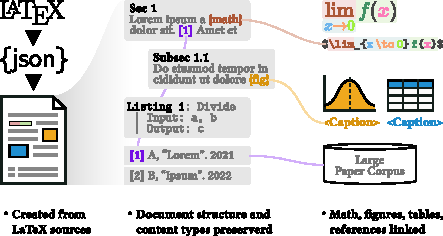
\includegraphics[width=\linewidth]{figures/ref_covgran/schema}
  % \caption{Schematic of our data set.\\
  %   \footnotesize\normalfont Created from arXiv.org \LaTeX\ sources, our data set preserves document \emph{sctructure} (sections, subsections, ...) and \emph{content types} (paragraphs, listings, ...). In-text positions of mathematical notation, figures, tables and citation markers are linked to \LaTeX\ math content, figure/table captions, and bibliographic references respectively. Bibliographical references are linked to the large paper corpus OpenAlex.
  % }
  \caption[Schematic of our data set]{Schematic of our data set. (Created from arXiv.org \LaTeX\ sources, our data set preserves document sctructure (sections, subsections, ...) and content types (paragraphs, listings, ...). In-text positions of mathematical notation, figures, tables and citation markers are linked to \LaTeX\ math content, figure/table captions, and bibliographic references respectively. Bibliographical references are linked to the large paper corpus OpenAlex.}
  \label{fig:schema}
\end{figure}

% - - - - - What are key shortcomings of current data sets? (research gap)

Key aspects of such data sets are (1)~basic measures such as quality, size, and temporal as well as disciplinary coverage, (2)~their citation network, and (3)~handling of non-textual content. (1)~Quality is affected by the source material (e.g. PDF or \LaTeX) and parsing method. (2)~The citation network is important to allow for bibliometric analyses. (3)~Non-textual content such as tables, figures, and mathematical notation often contain important information.

Across these key aspects, we see significant shortcomings in currently available data sets, as shown in Table~\ref{tab:comparison}. For example, (1)~limited size (SciXGen), (2)~omission of a citation network (arXMLiv), and (3)~no or limited handling of mathematical notation (S2ORC, unarXive 2020).

% NOTES
%
% S2ORC (PDF) math
% - convert to unicode -> error-prone & limited
%
% SciXGen
% - focus on text generation
% - demo domain expired, undocumented data on GitHub
% - https://aclanthology.org/2021.findings-emnlp.128/
% - https://github.com/sairin1202/SciXGen
%
%
% PMC-OAS
% get file list CSVs from here: https://ftp.ncbi.nlm.nih.gov/pub/pmc/oa_bulk/oa_comm/xml/
% $ ls oa_comm_xml.PMC00*xxxxxx.baseline.2023-02-08.filelist.csv
%    oa_comm_xml.PMC000xxxxxx.baseline.2023-02-08.filelist.csv
%    oa_comm_xml.PMC001xxxxxx.baseline.2023-02-08.filelist.csv
%    oa_comm_xml.PMC002xxxxxx.baseline.2023-02-08.filelist.csv
%    oa_comm_xml.PMC003xxxxxx.baseline.2023-02-08.filelist.csv
%    oa_comm_xml.PMC004xxxxxx.baseline.2023-02-08.filelist.csv
%    oa_comm_xml.PMC005xxxxxx.baseline.2023-02-08.filelist.csv
%    oa_comm_xml.PMC006xxxxxx.baseline.2023-02-08.filelist.csv
%    oa_comm_xml.PMC007xxxxxx.baseline.2023-02-08.filelist.csv
%    oa_comm_xml.PMC008xxxxxx.baseline.2023-02-08.filelist.csv
%    oa_comm_xml.PMC009xxxxxx.baseline.2023-02-08.filelist.csv
% $ cat oa_comm_xml.PMC00*xxxxxx.baseline.2023-02-08.filelist.csv | wc -l
%    3296051

% - - - - - How is this research gap closed? (conceptional) - - - - -

To address these issues, we propose a new version of the data set unarXive, %\footnote{The \LaTeX\ based data set for NLP on Academic Text}
which comprises 1.9 M publication across several disciplines, includes a more complete citation network than its predecessors, and retains structured mathematical notation as well as table and figure captions (see Figure~\ref{fig:schema}).  % captions = “textual surrogates”
Apart from the data set itself, we furthermore provide ready-to-use training and test data for two NLP tasks. Overall, we make the following contributions.

% - - - - - List of contributions, shared data, etc. (name numbers, facts, links to data, etc.) - - - - -

\begin{itemize}
    \item We provide a 1.9 M document scholarly data set, containing structured full-text, annotated in-text citations, linked table and figure captions, structured mathematical notation, and a hight quality citation network.
    \item We provide ready-to-use training/test data for the development and evaluation of approaches to two NLP tasks, namely citation recommendation and IMRaD classification.
    \item We distribute our data in accordance to the FAIR principles~\cite{Wilkinson2016} and share our source code freely available under a permissive license.
\end{itemize}

\afterpage{  % - - - start of afterpage
\begin{landscape}
\begin{table}
  % \caption{
  %   Comparison of large data sets derived from paper full-texts\\
  %   {\footnotesize\normalfont
  %    $^\dagger$Cit. network completeness is reported is two ways. ``general'': the whole data set; not directly comparable. ``compare'': for arXiv.org data from 1991--2020; directly comparable.\\
  %    $^\ddagger$References in the PMC-OAS are partially linked to a mixed set of IDs (PubMed, MEDLINE, DOI)~\cite{Gipp2015}. Therefore there is no single, comprehensive number for its completeness.
  %   }
  %  }
  \caption[Comparison of large data sets derived from paper full-texts]{Comparison of large data sets derived from paper full-texts ($^\dagger$Cit. network completeness is reported is two ways. ``general'': the whole data set; not directly comparable. ``compare'': for arXiv.org data from 1991--2020; directly comparable. $^\ddagger$References in the PMC-OAS are partially linked to a mixed set of IDs (PubMed, MEDLINE, DOI)~\cite{Gipp2015}. Therefore there is no single, comprehensive number for its completeness.}
  \label{tab:comparison}
  \begin{tabular}{lccccccccc}
    \toprule
    \ & \multicolumn{2}{c}{Source} & \multicolumn{2}{c}{\hphantom{wi}Citation Network$^\dagger$} & \multicolumn{2}{c}{Structured} & \ & \ & \ \\
    Data Set & Data & Format & general & compare & Doc. & Math. & \# Docs & Disciplines & Purpose \\
    \midrule
    CORE~\cite{core} & multiple & PDF & 0\% & - & $\times$ & $\times$ & $>$100 M & various & general NLP \\
    S2ORC (PDF)~\cite{Lo2020} & multiple & PDF & 69.4\% & - & \checkmark & $\times$ & 12 M & various & general NLP \\
    % (19.3+6.8)/(27.8+21.9) = 53% overall, 69.4% GROBID parses, 31.1% LaTeX parses
    unarXive 2020~\cite{Saier2020} & arXiv.org & \LaTeX & 42.6\% & 42.6\% & $\times$ & $\times$ & 1.2 M & phys., maths, CS & general NLP \\
    \midrule
    S2ORC (\LaTeX)~\cite{Lo2020} & arXiv.org & \LaTeX & 31.1\% & 31.1\% & \checkmark & \checkmark & 1.5 M & phys., maths, CS & general NLP \\
    arXMLiv~\cite{arXMLiv} & arXiv.org & \LaTeX & 0\% & 0\% & \checkmark & \checkmark & 1.6 M & phys., maths, CS & maths linguistics \\
    SciXGen~\cite{chen2021-scixgen} & arXiv.org & \LaTeX & 41.6\% & - & \checkmark & \checkmark & 205 k & CS & text generation \\
    PMC-OAS\textsuperscript{13} & PubMed & XML & mixed$^\ddagger$ & - & \checkmark & \checkmark & \textbf{3.3 M} & \textbf{biomedical} & not NLP specific \\  % TODO: make sure this footnotemark still is correct in the end, or convert the table to a threeparttable with its own tablenotes
    \textbf{unarXive 2022} (ours) & arXiv.org & \LaTeX & 44.4\% & \textbf{44.4\%} & \textbf{\checkmark} & \textbf{\checkmark} & \textbf{1.9 M} & \textbf{phys., maths, CS} & general NLP \\
    % 0.4441 for 1991—2022, 0.4438 for 1991–2020
    \bottomrule
  \end{tabular}
\end{table}
\end{landscape}
}  % - - - end of afterpage

\subsection{Related Work}

In Table~\ref{tab:comparison} we give an overview of related work.
Excluded are data sets that are either just sets of PDFs, or only contain metadata.

CORE~\cite{core}, while being very large, does not contain a citation network, nor is document structure preserved.
S2ORC (PDF)~\cite{Lo2020} is second in size and, while not directly comparable due to different publications covered, has the most complete citation network. However, mathematical notation is only partially preserved as plaintext.
unarXive 2020~\cite{Saier2020} has the second highest citation network completeness in direct comparison, but lacks structured content.

The bottom part of the table are data sets with both document structure preserved and structured mathematical notation.
S2ORC (\LaTeX)~\cite{Lo2020} is a discontinued\footnote{Last release including the \LaTeX\ subset is 2019-09-28, see \refurlinline{https://github.com/allenai/s2orc}{2023-02-12}.} subset of S2ORC and has a limited citation network, 
arXMLiv~\cite{arXMLiv} offers the highest level of structure but no citation network, and 
SciXGen~\cite{chen2021-scixgen} is limited in size.
The PMC-OAS~\refurl{https://www.ncbi.nlm.nih.gov/pmc/tools/openftlist/}{2023-11-06} is comparable to unarXive 2022 in size and structure, but has a partial and mixed citation network.


Overall, unarXive 2022 has the most complete citation network as far as direct comparison is possible, preserves document structure as well as structured mathematical notation, and is the largest data set covering physics, mathematics and computer science.

\subsection{Approach}
% How the data sets was created

We base our data set creation approach in part on S2ORC (\LaTeX) and in part on unarXive 2020. This is motivated as follows.

As shown in Table~\ref{tab:comparison}, the majority of related data sets is based on paper's \LaTeX\ sources---which is less noise-prone than parsing PDFs~\cite{Bast2017}. Among these, S2ORC (\LaTeX) provides well structured full-text content usable for a wide variety of applications (see Section~\ref{sec:applications}), while arXMLiv and SciXGen are optimized for special purposes. We therefore base our structured document representation on S2ORC (\LaTeX). Regarding the citation network, however, unarXive 2020 achieves the most high quality results in direct comparison among existing data sets. We therefore base our citation network creation on unarXive 2020.

Regarding both S2ORC (\LaTeX) and unarXive 2020, we don't just copy, but also improve upon the existing work. To furthermore provide an up-to-date data set, we use as source data all papers on arXiv.org up until the end of 2022.

Conceptually, our overall data set creation process can be broken down into two major steps, namely document parsing and reference linking, In the following these are described in more detail.

\subsubsection{Document Parsing}
To convert the \LaTeX\ source of a paper into a format that is well suited for NLP applications and analyses, we follow S2ORC (\LaTeX) and unarXive 2020 and perform the following three steps. First, we flatten the paper's \LaTeX\ source into a single \texttt{.tex} document using latexpand.\refurl{https://ctan.org/pkg/latexpand}{2023-11-10} Next, we use the tool Tralics\refurl{https://www-sop.inria.fr/marelle/tralics/}{2023-11-10} to convert the \LaTeX\ source into XML. In the last step, we create an easy to handle JSON structure from the XML.

We adapt and extend the JSON structure of S2ORC as shown in Table~\ref{tab:formext}. Adding paper metadata facilitates easier analyses (e.g. for specific or across disciplines). Including information on section numbers and types reflects the document structure more closely (e.g. the nesting structure is not lost). Retaining URLs from embedded links helps with reference linking (see Section~\ref{sec:reflink}).

We mark the position of citation markers, tables, figures, and mathematical notation within the running text, and link citations markers to their references, tables and figures to their captions (i.e., textual surrogates of their content), and mathematical notation to its original \LaTeX\ content.

\begin{table}
  \centering
  \caption{Extension of S2ORC format}
  \label{tab:formext}
  \begin{tabular}{p{2cm}p{5cm}p{6.5cm}}
    \toprule
    Entity & S2ORC data & Added data \\
    \midrule
    \textbf{Paper} &
        \begin{minipage}[t]{\linewidth}
            \begin{itemize}[nosep,after=\strut,leftmargin=1mm]
                \item ID
                \item abstract
                \item full-text (list of paragraphs)
                \item bibliographic references
            \end{itemize}
        \end{minipage} &
        \begin{minipage}[t]{\linewidth}
            \begin{itemize}[leftmargin=1mm]
                \item Metadata (title, list of authors, discipline, license, version history)
            \end{itemize}
        \end{minipage}\\
    %\midrule
    \textbf{Paragraph} &
        \begin{minipage}[t]{\linewidth}
            \begin{itemize}[leftmargin=1mm]
                \item Section title 
                \item text
            \end{itemize}
        \end{minipage} &
        \begin{minipage}[t]{\linewidth}
            \begin{itemize}[leftmargin=1mm]
                \item Section number 
                \item Section type (e.g. \textit{section}, \textit{subsection}) 
                \item Content type (e.g. \textit{paragraph}, \textit{listing}, \textit{proof})
            \end{itemize}
        \end{minipage}\\
    %\midrule
    \textbf{Bib\-li\-o\-gra\-phic reference} &
        \begin{minipage}[t]{\linewidth}
            \begin{itemize}[leftmargin=1mm]
                \item Parsed reference
                \item ID of cited document
            \end{itemize}
        \end{minipage} &
        \begin{minipage}[t]{\linewidth}
            \begin{itemize}[leftmargin=1mm]
                \item Raw reference string
                \item List of contained arXiv IDs
                \item List of embedded links (i.e. URLs of clickable links not rendered as text when viewing the document)
            \end{itemize}
        \end{minipage}\\
  \bottomrule
\end{tabular}
\end{table}

\subsubsection{Reference Linking}\label{sec:reflink}

To add a citation network to the data set, bibliographical references---which at this point are just raw strings of text---need to be associated with the cited documents they're referencing. We follow the methodology of unarXive 2020 and link references to a large corpus of publication metadata. To do this, references are first parsed to determine the contained information (title, authors, year, venue, etc.), which is then matched against the paper records in the large metadata corpus. For these two steps, we make the following changes and improvements of the unarXive 2020 approach.

\paragraph{Parsing} unarXive 2020 utilizes the tool Neural Parscit~\cite{neuralparscit} for reference parsing and furthermore uses a heuristic procedure to determine identifiers such as DOIs or arXiv IDs found within reference string. We use GROBID~\cite{Lopez2009}, a more commonly used and actively developed tool. Additionally, we extend the identifier determination heuristics to be more robust and versatile by refining matching patterns and extending them to more citation styles.

\paragraph{Matching} unarXive 2020 matches references to paper records in the Microsoft Academic Graph (MAG)~\cite{Sinha2015MAG}, which is no longer publicly available. Instead of the MAG, we use OpenAlex~\cite{openalex}, the MAG's open successor provided by the nonprofit organization OurResearch.\refurl{https://ourresearch.org/}{2023-11-10} Chosing OpenAlex allows us to also match references to recent papers, which would not be contained in legacy versions of the MAG. Additionally, the fact that OpenAlex paper records contain a variety of identifiers (e.g. DOI and PubMed ID) facilitates combined and comparative analyses of our data with others. Furthermore, OpenAlex has been deemed better suited for bibliographic analyses than the MAG~\cite{openalex-vs-mag}.

% if we need scientific foundation for the decision to choose OpenAlex:
% a recent research comparing MAG's and OpenAlex suitability for bibliometric work concludes: " OpenAlex seems to be more suited for bibliometric analyses than MAG"
% see: https://arxiv.org/abs/2206.14168 

% OpenAlex contains metadata on scholarly documents and related entities, such as authors and institutions. Regular (biweekly) updates, extensive coverage (of more than 247 million documents) and an emphasis on standardized document identifiers (, specifically DOI, PubMed ID and PMC ID,) make the use of OpenAlex for our reference matching promising~\cite{openalex}.

% OurResearch website: https://ourresearch.org/ (in footnote?)
% today: 247,826,959 documents in OpenAlex. Retrieved through API call: https://api.openalex.org/works 
% DOI rate: 143,111,972 of all docs have DOI maintained = 57\.8%
% for recent years much higher: 2020 : 0.74, 2021 : 0.86, 2022 : 0.98 (higher than in MAG)

\subsection{Results}

In the following, we first present key statistics of our proposed data set. Following that, we explain how the data set can be used for analyses as well as the development of NLP applications, and introduce training/test data for two NLP tasks. Lastly, we describe how the data set is distributed to facilitate easy adoption by the community of researchers and practitioners.

\subsubsection{Data Set}

% Stats and figures, exemplary findings/interesting obsevations as

Our data set comprises \emph{1,881,346 papers}, which contain a combined \emph{182,586,547} paragraphs, \emph{63,367,836 references} and \emph{133,744,613 in-text citation markers}. The distribution across disciplines is 57\% physics, 20\% mathematics, 17\% computer science, and a combined 5\% for others. %statistics, electrical engineering and systems science, quantitative biology, quantitative finance, and economics.
We are able to link 28,135,565 references (44.4\%) and 64,547,944 (48.3\%) in-text citation markers to OpenAlex. As shown in Table~\ref{tab:comparison}, this makes our citation network more complete than that of existing data sets.

In Listing~\ref{lst:datasample} we show an excerpt of our document representation for one paper, showcasing the extracted plain text and structured content.

\begin{lstlisting}[language=json,caption=Data example.,label=lst:datasample,breaklines=true,captionpos=b,frame=single,showlines=true,basicstyle=\tiny]
/* - - - - - - - example paper (arXiv:2105.05862) - - - - - - - */
{ "paper_id": "2105.05862",
  "metadata": {...},
  "abstract": {...},
  "body_text": [...],
  "ref_entries": {...},
  "bib_entries": {...} }
/* - - - - - - - one of the sections in body_text - - - - - - - */
{ "section": "Memory wave form",
  "sec_number": "2.1",
  "sec_type": "subsection",
  "content_type": "paragraph",
  "text": "The gauge choice leading us to this solution does not fix
           completely all the gauge freedom and an additional constraint
           should be imposed to leave only the physical degrees of freedom.
           This is done by projecting the source tensor {{formula:7fd88bcd-
           9013-433d-9756-b874472530d9}} into its transverse-traceless (TT)
           components (see for example {{cite:80dbb6c8b9c12f561a8e585faceac5f
           4e104d60d}}). Doing this and without loss of generality, we will
           use the following very well known ansatz for the source term
           proposed in {{cite:bc9a8ca19785627a087ae0c01abe155c22388e16}}\n" }
/* - - - - - - - ref_entries entry for {{formula:7fd88...}} - - - - - - - */
{ "latex": "S_{\\mu \\nu }",
  "type": "formula" }
/* - - - - - - - bib_entries entry for {{cite:80dbb...}} - - - - - - - */
{ "bib_entry_raw": "R. Epstein, The Generation of Gravitational Radiation by Esc
                    aping Supernova Neutrinos, Astrophys. J. 223 (1978) 1037.",
  "contained_links": [
    { "url": "https://doi.org/10.1086/156337",
      "text": "Astrophys. J. 223 (1978) 1037.",
      "start": 87,
      "end": 117 }
  ],
  "ids" {...} }
\end{lstlisting}

In Figure~\ref{fig:numpprs} we show the number of papers across all disciplines over all years covered. We can see that yearly arXiv.org submissions in computer science are likely to surpass those in physics in 2023. As a simple showcase of the use of structured full-text content, we show in Figure~\ref{fig:refdensity} how the average number of bibliographic references per paragraph developed over time for the three major disciplines represented in the data set. Dividing by paragraphs is done to account for variation in paper length. We can see that the density of references is increasing more rapidly in physics and computer science, than it is in mathematics.

\begin{figure}
  \centering
  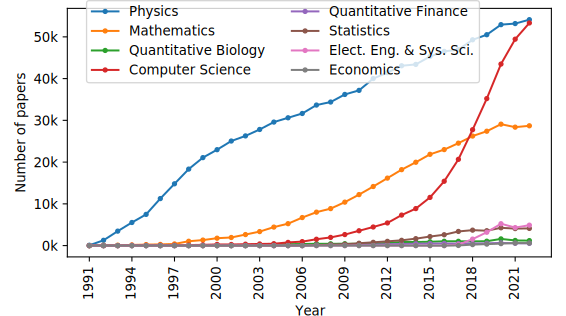
\includegraphics[width=0.7\linewidth]{figures/ref_covgran/numpprs}
  \caption{Number of papers per year.}
  \label{fig:numpprs}
% \end{figure}

% \begin{figure}
%   \centering
  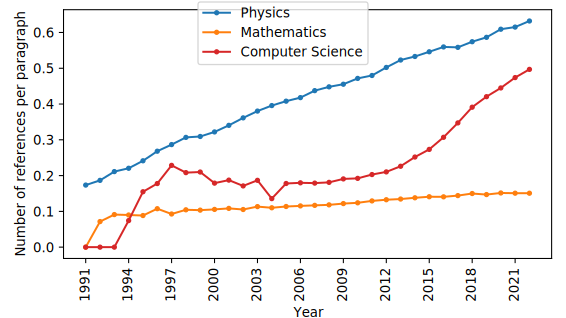
\includegraphics[width=0.7\linewidth]{figures/ref_covgran/refdensity}
  \caption{Reference density per year.}
  \label{fig:refdensity}
\end{figure}

% Physics: 1080760
% Mathematics: 380362
% Quantitative Biology: 16638
% Computer Science: 327207
% Quantitative Finance: 7933
% Statistics: 36717
% Electrical Engineering and Systems Science: 28212
% Economics: 3517

\subsubsection{Applications}\label{sec:applications}
% Applications and concrete examples how the research community benefits
% from this data set and what has been done to facilitate this

% \item Application cases/tasks
% \begin{itemize}
%     \item Citation recommendation
%     \item IMRaD classification
%     \item ...
% \end{itemize}

As is evident by the past use of our data set's predecessors unarXive 2020 and S2ORC, large-scale scholarly data sets created with NLP research in mind have broad applicability. Example uses are analyses of citation behavior across languages~\cite{Saier2021} or disciplines~\cite{Veneri2022} and the development of models for claim verification~\cite{wadden2020}, document retrieval~\cite{Parisot2022}, summarization~\cite{citesum}, or information extraction~\cite{viswanathan2021}.

Due to its similarities in structure and contained information, unarXive 2022 is equally suitable for the applications named above. Beyond these, we provide data for two NLP tasks on unarXive 2022, namely content based citation recommendation and IMRaD classification, which are described in the following.

\paragraph{Content Based Citation Recommendation}
Given a piece of text and a citation-marker position, the task of content based citation recommendation entails identifying publications which are suitable to cite in the given text at the given position~\cite{Bhagavatula2018,Faerber2020a}. Large full-text corpora of publications with a citation network provide a rich source for supervision of machine learning (ML) models for this task. That is, human made citations are used as training examples, or for evaluating models in a citation re-prediction setting.
From the premissively licensed papers in our data set we use all in-text citation markers with a linked reference cited at least three times, to allow splitting into train, dev, and test data.
The result is 2.5 M items consisting of (1) a paragraph and citation marker position (model input), and (2) the ID of the cited document (desired model output). % maybe add some stats on # of cited docs, etc.
% The data is available at \refurlinline{https://huggingface.co/datasets/saier/unarXive_citrec}.

\paragraph{IMRaD Classification}
Scientific publications are usually structured into sections commonly summarized as ``Introduction, Methods, Results, and Discussion'' (IMRaD). Classifying sections of scientific text into these four classes is done, for example, in fine-grained citation classification. % ---to answer, for example, if a publication was cited as background information in the introduction, or as an influence on the methodology in the methods section.
Because conventions differ between disciplines, we prepare data for this task for computer science papers only. To aforementioned four classes we add the common ``Related Work'' section as a fifth class. From the premissively licensed computer science papers in our data, we use those that are unambiguously assignable to one of the five classes. The result is 530~k items consisting of (1) the paragraph text (model input), and (2) the class (desired model output). An exemplary application scenario for a model trained on this data is a paper writing assistant that can detect parts in a manuscript, which might be better placed in a different section (e.g. discussion rather than results).
% The data is available at \refurlinline{https://huggingface.co/datasets/saier/unarXive_imrad_clf}{2023-11-10}.


% 277388 CS papers
% 1604694 non CS papers
% defaultdict(<class 'int'>,
%             {'discussion': 555271,
%              'introduction': 1826742,
%              'methods': 424280,
%              'other': 19323579,
%              'related_work': 385052,
%              'results': 273471})
% 3464816 IMRaDR papras

\subsubsection{Distribution}

% - Zenodo
% - Permissively licenced subset
%     - CC: 197315
%     - public domain: 9779
%     -> 207094
%     207094/1881346 = 11.0078 %
% - Huggingface dataloader

Under consideration of the FAIR principles, we chose the following well established distribution channels and licenses for our data set, aforementioned NLP task data, as well as our source code.

\begin{itemize}
    \item The \textbf{data set} is distributed on \texttt{Zenodo}.\\
        \begin{small}
        $\rightarrow$\refurlinline{https://doi.org/10.5281/zenodo.7752615}{2023-11-10} (open subset)\\
        $\rightarrow$\refurlinline{https://doi.org/10.5281/zenodo.7752754}{2023-11-10} (full)\\
        \end{small}
        In accordance with the licensing terms of our source data, we share our data set in two versions.\\
        (1) The subset generated from permissively licensed source data (165 k publications, 9\%) is openly accessible.\\
        (2) The full data set, generated partially from source data under arXiv.org's ``non-exclusive license to distribute,''\refurl{http://arxiv.org/licenses/nonexclusive-distrib/1.0/}{2023-11-10} is accessible through Zenodo's ``restricted access'' policy,\refurl{https://about.zenodo.org/policies/}{2023-11-10}
making it possible to grant access to the data on request given the intended use is in accordance with the license terms.
    \item The \textbf{NLP task data} is provided on the \texttt{Hugging Face Hub}.\\
        \begin{small}
        $\rightarrow$\refurlinline{https://hf.co/datasets/saier/unarXive_citrec}{2023-11-10}\\
        $\rightarrow$\refurlinline{https://hf.co/datasets/saier/unarXive_imrad_clf}{2023-11-10}\\
        \end{small}
        This facilitates easy access and use by the NLP community.
    \item The \textbf{source code} for creating the data set is shared on \texttt{GitHub} under the MIT License.\\
        \begin{small}
        $\rightarrow$\refurlinline{https://github.com/IllDepence/unarXive}{2023-11-10}\\
        \end{small}
        Sharing the code openly and permissively licensed allows anyone to freely modify and extend the code to their needs. This makes, for example, integration into other NLP projects such as benchmarks and frameworks possible.
\end{itemize}

\subsection{Conclusion}
We propose unarXive 2022, a data set generated from 1.9 M \LaTeX\ paper sources and suitable for a wide variety of analyses and NLP applications. We base our approach to data set creation and format on existing works, while also addressing their shortcomings. Improving upon these tried and tested predecessors, unarXive 2022 offers the most complete citation network and most structured content compared to existing data sets, and is surpassed in size only by the PMC-OAS, which covers a different set of disciplines.

With our data set we provide data for two NLP tasks, content based citation recommendation and IMRaD classification, to facilitate its usage. We furthermore distribute our work under consideration of the FAIR principles, sharing it through well established channels and permissively licensed, thereby ensuring proper accessibility, easy use, and possibilities for adaption and extension.

We plan to incrementally update our data set with new arXiv.org submissions. For future developments, we note the importance of mathematical notation in academic publications, as reflected by recent SemEval tasks in 2021 and 2022~\cite{semeval21_task8,semeval22_task12}. Similar to existing projects,\refurl{https://github.com/PierreSenellart/theoremkb}{2023-11-10} we plan to investigate novel analyses and applications based on the combination of our data set's citation network and structured mathematical notation.

% Possible addition: \cite{Meuschke2023} -> PDF extraction still struggles w/ mathematical notation across the board, so mathematical notation is not only important but also hard to get by

% Publications in many scientific disciplines communicate key information through numbers and formulae. Accordingly, the extraction of such information has recently gained attention~\cite{semeval21_task8,semeval22_task12}

% In [10]: np.sum(mtrs['num_para_type_proof'])
% Out[10]: 2014983.0

% \cite{delemazure2020}

\subsection*{Author Contributions}  % cf. https://credit.niso.org/
Tarek Saier: Conceptualization, Data curation (lead), Formal analysis, Methodology, Software (lead), Visualization, Writing -- original draft, Writing -- review \& editing. Johan Krause: Data curation (support), Software (support). Michael F{\"a}rber: Writing -- review \& editing.

%%
%% The acknowledgments section is defined using the "acks" environment
%% (and NOT an unnumbered section). This ensures the proper
%% identification of the section in the article metadata, and the
%% consistent spelling of the heading.
\subsection*{Acknowledgements}
This work was partially supported by the German Federal Ministry of Education and Research (BMBF) via [KOM,BI], a Software Campus project (01IS17042).
The authors acknowledge support by the state of Baden-W{\"u}rttemberg through bwHPC.
We thank Johannes Reber for supporting early stages of the software development.

\chapter{References Across Languages}
\label{chp:xling}

This chapter is based on the following publications.
\begin{quote}
\fullcite{Saier2020xling}\\
\\
\fullcite{Saier2021}
\end{quote}

% \begin{abstract}
% Citation information in scholarly data is an important source of insight into the reception of publications and the scholarly discourse. Outcomes of citation analyses and the applicability of citation based machine learning approaches heavily depend on the completeness of such data. One particular shortcoming of scholarly data nowadays is that non-English publications are often not included in data sets, or that language metadata is not available.
% Because of this, citations between publications of differing languages (cross-lingual citations) have only been studied to a very limited degree. In this paper, we present an analysis of cross-lingual citations based on over one million English papers, spanning three scientific disciplines and a time span of three decades.
% Our investigation covers differences between cited languages and disciplines, trends over time, and the usage characteristics as well as impact of cross-lingual citations. Among our findings are an increasing rate of citations to publications written in Chinese, citations being primarily to local non-English languages, and consistency in citation intent between cross- and monolingual citations.
% To facilitate further research, we make our collected data and source code publicly available.
% \end{abstract}

\section{Introduction}

\begin{figure}[tb]
\centering
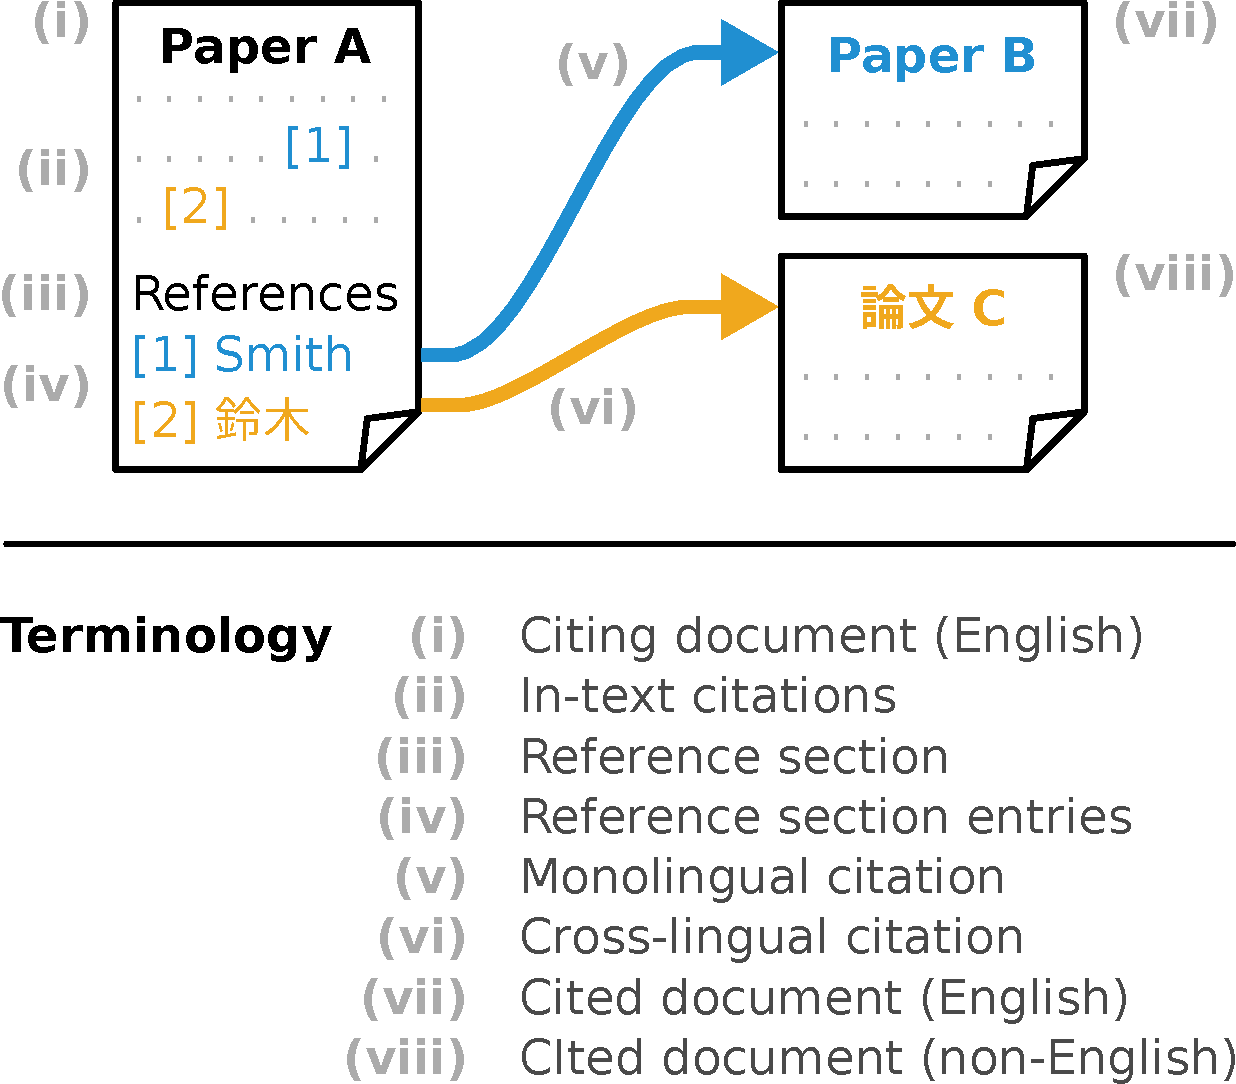
\includegraphics[width=0.5\linewidth]{figures/ref_xling/terminology_with_text_twocolumn.pdf}
\caption{Schematic explanation of terminology.} \label{fig:terminology}
\end{figure}

Citations are an essential tool for scientific practice. By allowing authors to refer to existing publications, citations make it possible to position one's work within the context of others', critique, compare, and point readers to supplementary reading material. In other words, citations enable scientific discourse. Because of this, citations are a valuable indicator for the academic community's reception of and interaction with published works. Their analysis is used, for example, to quantify research output~\cite{Hirsch2005}, qualify references~\cite{Abujbara2013}, and detect trends~\cite{Chen2006}. Furthermore, citations can be utilized to aid researchers through, for example, summarization~\cite{Elkiss2008} or recommendation~\cite{Ma2020,Faerber202x} of papers, and through applications driven by document embeddings in general~\cite{Cohan2020}.

As such analyses and applications require data to be based on, the availability of citation data or lack thereof is decisive with regard to the areas, in which respective insights can be gained and approaches developed. Here, the literature points 
in two major directions of lacking coverage---namely the humanities~\cite{Colavizza2019,Kellsey2004} and non-English publications~\cite{Vera-Baceta2019,Liu2019,Moed2018,Moskaleva2019}.
Because most large scholarly data sets are either artificially limited to few languages (e.g., English only) or do not provide language metadata,
a particular practice not well researched so far is cross-lingual citation. That is, references where the citing and cited documents are written in different languages (see \textit{(vi)} in Figure~\ref{fig:terminology}).
Cross-lingual citations are, however, important bridges between otherwise insufficiently connected ``language silos''~\cite{Shu2019,Moskaleva2019}.

Because English is currently the de facto academic lingua franca~\cite{Montgomery2013}, citations from non-English languages to English are significantly more prevalent than the other way around. This dichotomy is reflected in existing literature, where usually either citations from English~\cite{Kellsey2004,Lillis2010}, or to English~\cite{Tang2014,Jiang2018,Jiang2018b,Schrader2019} are analyzed. As both directions involve a non-English document on one side of the citation, the analysis of either is challenging with today's Anglocentric state of citation data.

Setting our focus to cross-lingual citations \emph{from English}, we perform a large-scale analysis on over one million documents.
In line with existing literature we determine the prevalence of cross-lingual citations across multiple dimensions. Additionally, we investigate the citation's usage as well as impact. In particular, the following research questions are addressed.

\begin{enumerate}[align=left]
\item[RQ1)] How prevalent are English to non-English references? We consider prevalence in general, in different disciplines, across time, and within publications that use them.
\item[RQ2)] In what circumstances are cross-lingual citations in English papers used? Here we consider self-citation, geographic origin, as well as citation function and sentiment.
\item[RQ3)] What is the impact of cross-lingual citations in English documents? We consider the aspects of acceptance, data mining challenges, as well as impact on the success of a publication.
\end{enumerate}

\noindent Through our analysis, we make the following contributions.

\begin{enumerate}
\item We conduct an analysis of cross-lingual citations in English papers that is considerably more extensive than existing literature in terms of corpus size as well as covered languages, time, and disciplines. This not only makes the results more representative of the areas covered, but also enables the use of our collected data for machine learning based applications such as cross-lingual citation recommendation.
\item We propose an easy and reliable method for identifying cross-lingual citations from English papers to publications in non-Latin script languages (e.g., Russian and Chinese).
\item We highlight key challenges for handling cross-lingual citations that can inform future developments in scholarly data mining.
\item To facilitate further research, we make our collected data, source code, and full results publicly available.\footnote{See \url{https://github.com/IllDepence/cross-lingual-citations-from-en}.}
\end{enumerate}

\noindent The remainder of the paper is structured as follows. After briefly addressing our use of terminology down below, we give an overview of related work in Section~\ref{sec:relwork}. In Section~\ref{sec:datacollection} we discuss the identification of cross-lingual citations, data sources considered, and our data collection process. Subsequent analyses with regard to our research questions are then covered in Section~\ref{sec:results}. We end with a discussion of our findings and concluding remarks in Section~\ref{sec:xling-conclusion}.

\subsection*{Terminology}
Because \textit{citation}, \textit{reference} and related terms are not used consistently in literature, we briefly address their use in this paper. As shown in Figure~\ref{fig:terminology}, a cit\emph{ing} document creates a bibliographical link to a cit\emph{ed} document. We use the terms \textit{citation} and \textit{reference} interchangeably for this type of link (e.g., ``\textit{(vi)} in Figure~\ref{fig:terminology} marks a cross-lingual reference,'' or ``Paper$^a$ makes two citations''). The textual manifestation of a bibliographic reference, often found at the end of a paper (e.g., ``[1] Smith'' in Figure~\ref{fig:terminology}), is referred to as \textit{reference section entry}, or sometimes \textit{reference} for short. We call the combined set of these entries \textit{reference section}. Lastly, parts within the text of a paper, which contain a marker connected to one of the reference section entries are called \textit{in-text citations}.

\section{Related Work}\label{sec:relwork}

\begin{table*}
\caption{Comparison of corpora}
 \label{tab:relworkcomp}
  \centering
  \begin{small}
 \begin{threeparttable}
 \begin{tabular}{lcrrrr}
 \toprule
   Work & Type\tnote{a} & \#Docs & \hphantom{m}\#References & \hphantom{m}\#Years & \hphantom{nn}\#Disciplines \\
   \midrule
   Kellsey and Knievel~\cite{Kellsey2004} & en$\rightarrow$* & 468 & 16k & 5\tnote{b} & 4 \\
   Lillis et al.~\cite{Lillis2010} & en$\rightarrow$* & 240 & 10k & 7 & 1 \\
   Schrader~\cite{Schrader2019} & *$\rightarrow$en & 403 & 5k & 2 & 1 \\
   Tang et al.~\cite{Tang2014} & zh$\rightarrow$en & 2k & 17k & 10 & 1 \\
   Jiang et al.~\cite{Jiang2018,Jiang2018b} & zh$\rightarrow$\{en,zh\} & 14k & 38k & n/a & 1 \\
   Kirchik et al.~\cite{Kirchik2012} & \{en,ru\}$\rightarrow$ru & 497k & n/a & 17 & (unrestricted) \\
   Ours & en$\rightarrow$* &  1.1M & 39M & 27 & 3 \\
   \bottomrule
 \end{tabular}
 \begin{tablenotes}
    \item[a] type$=$focus reference type (en$=$English, ru$=$Russian, zh$=$Chinese, *$=$any)
    \item[b] over a span of 40 years
 \end{tablenotes}
\end{threeparttable}
  \end{small}
\end{table*}

Existing literature on cross-lingual citations in academic publications covers analyses as well as approaches to prediction tasks. These are, however, only based on small corpora or restricted to specific language pairs. As shown in Table~\ref{tab:relworkcomp}, our work is based on a considerably larger corpus which is also more comprehensive in terms of the time span and disciplines that are covered.

In the following, we describe the works in Table~\ref{tab:relworkcomp} in more detail, reporting on the key corpus characteristics and findings. This is complemented by a short overview of existing literature on various types of cross-lingual interconnections in media other than academic publications.


\subsection{Cross-Lingual Citations in Academic Publications}

Literature concerning cross-lingual citations in academic publications can be found in the form of analyses and applications. In \cite{Kellsey2004} Kellsey and Knievel conduct an analysis of 468 articles containing 16,138 citations. The analysis spans 4 English language journals in the humanities (disciplines: history, classics, linguistics, and philosophy) over 5 particular years (1962, 1972, 1982, 1992, and 2002). They count cross-lingual citations to English, German, French, Italian, Spanish, Portuguese, and Latin, while further languages are grouped into a category ``other.''
The authors find that 21.3\% of the citations in their corpus are cross-lingual, but note strong differences between the covered disciplines. Over time, they observe a steady total, but declining relative number of cross-lingual citations per article. The authors furthermore find, that the ratio of publications that contain at least one cross-lingual citation is increasing.

Lillis et al.~\cite{Lillis2010} investigate if the global status of English is impacting the ``citability'' of non-English works in English publications. They base their analysis on 240 articles from 2000 to 2007 in psychology journals, and furthermore use the Social Sciences Citation Index and ethnographic records. Their corpus contains 10,688 references, of which 8.5\% are cross-lingual. Analyzing the prevalence of references in various contexts, they find that authors are more likely to cite a ``local language'' in English-medium national journals than in international journals. Further conducting analyses of e.g. in-text citation surface forms, they come to the conclusion that there are strong indicators for a pressure to cite English rather than non-English publications.

Similar observations are made by Kirchik et al.~\cite{Kirchik2012} concerning citations to Russian. Analyzing 498,221 papers in Thomson Reuters' Web of Science between 1993 and 2010, they find that Russian scholars are more than twice as likely to cite Russian publications when publishing in Russian language journals (21\% of citations) than when they publish in English (10\% of citations).

In \cite{Schrader2019} Schrader analyzes citations from non-English documents to English articles in open access and ``traditional'' journals. The corpus used comprises 403 cited articles published between 2011 and 2012 in the discipline of library and information science. The articles were cited 5,183 times (13.8\% by non-English documents). In their analysis the author observes that being open access makes no statistically significant difference for the ratio of incoming cross-lingual citations of an article, or the language composition of citations a journal receives.

Apart from analyses, there are also approaches to prediction tasks based on cross-lingual citations~\cite{Tang2014,Jiang2018,Jiang2018b,Ma2020}. Tang et al.~\cite{Tang2014} propose a bilingual context-citation embedding algorithm for the task of predicting suitable citations to English publications in Chinese sentences. To train and evaluate their approach, they use 2,061 articles from 2002 to 2012 in the Chinese Journal of Computers, which contain citations to 17,693 English publications. Comparing to several baseline methods, they observe the best performance for their novel system. Similarly, in \cite{Jiang2018} and \cite{Jiang2018b} Jiang et al. propose two novel document embedding methods jointly learned on publication content and citation relations. The corpus used in both cases consists of 14,631 Chinese computer science papers from the Wanfang digital library. The papers contain 11,252 references to Chinese publications and 27,101 references to English publications. For the task of predicting a list of suitable English language references for a Chinese query document, both approaches are reported to outperform a range of baseline methods.

\subsection{Cross-Lingual Interconnections in Other Types of Media}

Apart from academic publications, cross-lingual connections are also described in other types of media. Hale~\cite{Hale2012} analyzes cross-lingual hyperlinks between online blogs centered around a news event in 2010. In a corpus of 113,117 blog pages in English, Spanish, and Japanese, 12,527 hyperlinks (5.6\% of them cross-lingual) are identified. Analysis finds that less than 2\% of links in English blogs are cross-lingual, while the number in Spanish and Japanese blogs is slightly above 10\%. Hyperlinks between Spanish and Japanese are almost non-existent (7 in total). Further investigating the development of links over time, the author observes a gradual decrease in language group insularity driven by individual translations of blog content---a phenomenon described as ``bridgeblogging'' by Zuckerman~\cite{Zuckerman2008}.
Similar structural features are reported by Eleta et al.~\cite{Eleta2012} and Hale~\cite{Hale2014a} for Twitter, where multilingual users are bridging language communities.

Focusing on types of information diffusion that are not textually manifested through connections such as bibliographic references and hyperlinks, there also is literature on cross-lingual phenomena on collaborative online platforms, such as the study of cross-lingual information diffusion on Wikipedia~\cite{Kim2016,Samoilenko2016}.

Lastly, as with academic publications, there furthermore exists literature on link prediction tasks. In \cite{Jin2017} Jin et al. analyze cross-lingual information cascades and develop a machine learning approach based on language and content features to predict the size and language distribution of such cascades.

\section{Data Collection}\label{sec:datacollection}

In this section, we first discuss how to identify cross-lingual citations. Subsequently, we outline the steps of data source selection and corpus construction. Lastly, we describe the key characteristics of our corpus.

\subsection{Identification of Cross-Lingual Citations}
\label{sec:ident}
Identifying cross-lingual citations requires information about the language of the citing and cited document. However, this is often missing in scholarly data sets.\footnote{Details are provided in Section~\ref{sec:dataselect}.} Identifying the involved documents' language when it is not given in metadata, however, is challenging, because (a) the full text, especially of the cited documents, is not always available, (b) abstracts are not reliable because non-English publications often provide an additional English abstract, and (c) language identification on short strings (e.g., titles in references) does not achieve sufficient results with existing techniques~\cite{Jauhiainen2019}.

To nevertheless be able to conduct an analysis of cross-lingual citations on a large scale, we utilize the common practice of authors appending an explicit marker in the form of \textit{``(in $<$Language$>$)''} to such references. This shifts the requirements from language metadata or language identification to the existence of reference section entries in the data. This is because the language of the cited document is given by the \textit{``$<$Language$>$''} part of the marker, and the language the marker itself is written in (i.e., English) provides the citing document's language. For example, the reference section entry \textit{``M. Saitou, `Hydrodynamics on non-commutative space' (in Japanese), [...]''}\footnote{Found in \texttt{arXiv:1612.01831}.} by itself contains enough information to determine that the cited document is written in Japanese and the citing document is written in English.

The question then remains, how common the practice of using such explicit markers is---that is, to cite, for example, \textit{``A Modern Model Description of Magnetism (in Russian)''} instead of \textit{``\foreignlanguage{russian}{Современное модельное описание магнетизма}''}.\footnote{Referring to \texttt{arXiv:1103.5123}.} To answer this question, we perform a preliminary analysis on the data set unarXive~\cite{Saier2020}, which comprises 39 million reference section entries. Specifically, we conduct a large automated analysis on all reference section entries in the data set and additionally perform a smaller, manual analysis on a stratified sample of 5,000 references.

In the large automated analysis, we first identify the cited document's title within references using the state-of-the-art~\cite{Tkaczyk2018} reference string parser module of GROBID~\cite{Lopez2009}, and then determine the title's language using the language identification tool Lingua,\footnote{See \url{https://github.com/pemistahl/lingua}.} which is specialized for very short text.
Manually inspecting our results, we note that non-Latin script languages (e.g., Chinese, Japanese, Russian) are detected reliably,\footnote{To be more precise, no language that uses a script different to the Latin alphabet appears to be falsely identified as English. We are, however, not able to judge whether languages using the same non-Latin script---such as languages written in Cyrillic---are distinguished correctly by Lingua.} but Latin script languages (e.g., German and French) are not. For instance, many English titles are falsely identified as German.

\begin{table}
\caption{References to non-Latin script languages in the automated analysis}
 \label{tab:automatedresults}
  \centering
  \begin{small}
 \begin{threeparttable}
 \begin{tabular}{lrr}
 \toprule
   Cited Language & \#marked & \#unmarked \\
   \midrule
   Russian & 23,922 & 303 (1.3\%)\\
   Chinese & 2,351 & 10 (0.4\%) \\
   Japanese & 1,843 & 5 (0.3\%) \\
   Ukrainian & 876 & 15 (1.7\%)\\
   Bulgarian & 67 & 0 (0.0\%)\\
   Greek & 60 & 1 (1.7\%) \\
   \bottomrule
 \end{tabular}
\end{threeparttable}
  \end{small}
\end{table}

For non-Latin script languages, which we is shown in Table~\ref{tab:automatedresults}, only a small fraction of cross-lingual citations is not explicitly marked. We observe ratios of unmarked cross-lingual citations relative to explicit markers consistently below 2\%.\footnote{Because our analysis is based on language identification of the titles of cited publications, we cannot detect when a non-English work is cited with a translated title \emph{and} no explicit language marker.}

\begin{table}
\caption{Results of manual labeling}
 \label{tab:manualresults}
  \centering
  \begin{small}
 \begin{threeparttable}
 \begin{tabular}{lrr}
 \toprule
   Cited Language & \#references & \#marked \\
   \midrule
   (n/a)\tnote{a} & 2,737 & 0 \\
   English & 2,188 & 0 \\
   French & 33 & 1 \\
   German & 27 & 0 \\
   Russian & 8 & 6\tnote{b}\\
   Italian & 5 & 1 \\
   Chinese & 1 & 1 \\
   Japanese & 1 & 1 \\
   \bottomrule
 \end{tabular}
 \begin{tablenotes}
    \item[a] These references did not contain the title of the cited document, which is common in physics papers.
    \item[b] The two remaining unmarked references contained the cited publication's title only transliterated into the Latin alphabet.
  \end{tablenotes}
\end{threeparttable}
  \end{small}
\end{table}

To get a reliable estimate for Latin script languages as well, we additionally perform a smaller, manual analysis. To this end, we label a stratified sample\footnote{The sample was stratified according to the referencing document's discipline and month of publication.} of 5,000 references from unarXive with the reference's language as well as whether an explicit language marker was used or not. The results of our evaluation are shown in Table~\ref{tab:manualresults}.
In accordance with our automated large analysis, we observe that non-Latin script languages are generally explicitly marked. For Latin script languages, however, explicit marking appears to be considerably less common. We additionally evaluate the automated language identification results for our manually annotated references and measure F1 scores of 0.48, 0.46, and 0.60 for French, German, and Italian respectively. Notably, less than half of the references with German titles are detected (44\% recall) and more than half of the references identified as German are false positives (48\% precision).

The results of above preliminary investigations have two consequences for the findings in our main analyses, which are based on explicit language markers. First, a direct comparison between our results on non-Latin and Latin script languages is only valid for \emph{explicitly marked} cross-lingual citations, as there is a notable amount of undetected cross-lingual citations for Latin script languages. Second, the number of undetected cross-lingual citations for non-Latin script languages such as Chinese, Japanese, and Russian, is negligible. Accordingly, concerning these languages, our results are valid for cross-lingual citations \emph{regardless of language markers}.

\subsection{Data Source Selection}\label{sec:dataselect}

\begin{table}
\caption{Overview of data sets}
 \label{tab:datasets}
  \centering
  \begin{small}
 \begin{threeparttable}
 \begin{tabular}{lrlllc}
 \toprule
   Data set & \#Docs & Lang. Meta\tnote{a} & Refs. to\tnote{b} & Reference sections & Used \\
   \midrule
   MAG\tnote{c}~~\cite{Sinha2015,Wang2019} & 230M  & (48\%\tnote{d}~) & MAG & - & \checkmark\\
   CORE\tnote{e} & 123M & 1.79\% & CORE & - & \\
   S2ORC~\cite{Lo2020} & 81M & - & S2ORC & 34\% (in GROBID parse) & \\
   PubMed Central OAS\tnote{f} & 2M & - & mixed & 100\% (in JATS XML) & \\
   unarXive~\cite{Saier2020} & 1M & - & MAG & 100\% (dedicated entity) & \checkmark\\
   \bottomrule
 \end{tabular}
 \begin{tablenotes}
    \item[a] Language metadata
    \item[b] References resolved to
    \item[c] Using version 2019-12-26
    \item[d] Language given for source URLs (not always matching paper language)
    \item[e] See \url{https://core.ac.uk/}. Using version 2018-03-01
    \item[f] See \url{https://www.ncbi.nlm.nih.gov/pmc/tools/openftlist/}
  \end{tablenotes}
\end{threeparttable}
  \end{small}
\end{table}

As our data source we considered five large scholarly data sets commonly used for citation related tasks~\cite{Khan2017,Faerber202x}. Table~\ref{tab:datasets} gives an overview of their key properties. The Microsoft Academic Graph (MAG) and CORE are both very large data sets with some form of language metadata present. In the MAG the language is given not for documents themselves, but for URLs associated with papers. CORE contains a language label for 1.79\% of its documents. S2ORC, the PubMed Central Open Access Subset (PMC OAS), and unarXive do not offer language metadata, but all contain some form of reference sections (GROBID output, JATS~\cite{Huh2014} XML, and raw strings extracted from \LaTeX~source files respectively).

From these five, we decided to use unarXive and the MAG. This decision was motivated by two key reasons: (1)~metadata of cited documents, and (2)~evaluation of the acceptance of cross-lingual citations in English papers. As for (1), both S2ORC and the PMC OAS link references in their papers to document IDs within the data set itself (only partly in the PMC OAS, where also MEDLINE IDs and DOIs are found~\cite{Gipp2015}). This is problematic in our case, because S2ORC is restricted to English papers, and the PMC OAS is constrained to Latin script contents,\footnote{See \url{https://www.ncbi.nlm.nih.gov/pmc/about/faq/\#q16}.} which means metadata on non-English cited documents is non-existent (S2ORC) or very limited (PMC OAS). In unarXive, on the other hand, references are linked to the MAG, which contains metadata on publications regardless of language. Concerning reason (2), the fact that unarXive is built from papers on the preprint server arxiv.org, and the MAG contains metadata on paper's preprint \emph{and} published versions, allows us to analyze whether or not cross-lingual citations are affected by the peer review process.

With these two data sources selected, the extent of our analysis is over one million documents, across 3 disciplines (physics, mathematics, computer science), over a span of 27 years (1992--2019).

\subsection{Data Collection}\label{sec:datacollectionsub}
To identify references with \textit{``(in $<$Language$>$)''} markers, we iterate through the total of 39.7M reference section entries in unarXive and first filter for the regular expression \verb|\(\s*in\s+[a-zA-Z][a-z]+\s*\)|. This yields 51,380 matches with 207 unique tokens following \textit{``in''} within the parentheses. Within these 207 tokens we manually remove those referring to non-languages (e.g., ``press'' or ``preparation'') and correct misspellings (e.g., ``japanease'' or ``russain''), resulting in 44 unique language tokens. These are (presented in ISO 639-1 codes) be, bg, ca, cs, da, de, el, en, eo, es, et, fa, fi, fr, he, hi, hr, hu, hy, id, is, it, ja, ka, ko, la, lv, mk, mr, nl, no, pl, pt, ro, ru, sa, sk, sl, sr, sv, tr, uk, vi, and zh. These 44 languages cover 43 of the 78 languages, in which journals indexed in the Directory of Open Access Journals\footnote{See \url{https://doaj.org/}.} (DOAJ) are published as of July 2020. The one language found in our data, but with no journal in the DOAJ, is Marathi. In terms of journal count by language, above 44 languages cover 97.54\% of the DOAJ. In total, our data contains 33,290 reference section entries in 18,171 unique citing documents. We refer to this set of documents as the \emph{cross-lingual set}.

To analyze differences between papers containing cross-lingual citations in unarXive and a comparable random set, we also generate a second set of papers. To ensure comparability we go through each year of the cross-lingual set, note the number of documents per discipline and then randomly sample the same number of documents from all of unarXive within this year and discipline. This means the \emph{cross-lingual set} and the \emph{random set} have the same document distribution across years and disciplines. Table \ref{tab:dataused} gives an overview of the resulting data used.

\section{Results}\label{sec:results}

In the following we describe the results of our analyses with regard to the research questions laid out in the introduction. We begin with general numbers concerning the \emph{prevalence} of cross-lingual citations. These results are based on unarXive alone. This is followed by more in depth observations regarding cross-lingual citations' \emph{usage} (e.g., the underlying motivation or the citation's function) and \emph{impact} (e.g., acceptance by reviewers or challenges for data mining). These subsequent in depth analyses additionally utilize the MAG metadata.

\begin{table}
\caption{Overview of data used}
 \label{tab:dataused}
  \centering
  \begin{small}
 \begin{threeparttable}
 \begin{tabular}{lrrr}
 \toprule
   \multicolumn{2}{r}{Cross-lingual set} & Random set & unarXive \\
   \midrule
   \#Docs & 18,171 & 18,171 & 1,192,097 \\
   \#Docs (MAG) & 16,300 & 16,464 & 1,087,765 \\
   \#Refs & 635,154 & 536,672 & 39,694,083 \\
   \#Refs (MAG) & 290,421 & 242,090 & 15,954,664 \\
   \#Cross-lingual refs & 33,290 & 642 & 33,290 \\
   \bottomrule
 \end{tabular}
 \begin{tablenotes}
    \item *docs  =  documents,\\\hphantom{*}refs  =  reference section entries,\\\hphantom{*}(MAG) = with a MAG ID.
  \end{tablenotes}
\end{threeparttable}
  \end{small}
\end{table}

\subsection{Prevalence}

We find \textit{``(in $<$Language$>$)''} markers in 33,290 out of 39,694,083 reference section entries (0.08\%). These appear in 18,171 out of 1,192,097 documents (1.5\%)---in other words in every 66th document. Of these 18k documents, 17,223 cite one language other than English, 864 cite two, 76 three, 7 documents four, and a single document cites works in English and five further languages (Russian, French, Polish, Italian, and German). The five most common language pairs within a single document are Russian-Ukrainian (277 documents), German-Russian (166), French-Russian (135), French-German (68), and Chinese-Russian (59).

\begin{table}
\caption{Most prevalent languages}
 \label{tab:prevlangs}
  \centering
  \begin{small}
 \begin{threeparttable}
 \begin{tabular}{lrr}
 \toprule
   Language & \#References & \#Documents \\
   \midrule
   Russian & 23,922 & 12,304 \\
   Chinese & 2,351 & 1,582 \\
   Japanese & 1,843 & 1,397 \\
   German & 1,244 & 965 \\
   French & 931 & 719 \\
   \bottomrule
 \end{tabular}
\end{threeparttable}
  \end{small}
\end{table}

Table~\ref{tab:prevlangs} shows the absolute number of reference section entries and unique citing documents for the five most prevalent languages, which combined make up over 90\% in terms of both references and documents. As we can see, Russian is by far the most common, making up about two thirds of the cross-lingual set. When breaking down these numbers by year or discipline, it is important to also factor in the distribution of documents along these dimensions in the whole data set. Doing so, we show in Figure~\ref{fig:previntime} the relative number of documents with cross-lingual citations over time for each of the aforementioned five languages. While the numbers in earlier years can be a bit unstable due to low numbers of total documents, we can observe a downwards trend of citations to Russian, an upwards trend of citations to Chinese, and a somewhat stable proportion in documents citing Japanese works. Looking at the numbers per discipline in Figure~\ref{fig:prevperdisc}, we can see that cross-lingual citations occur most often in mathematics papers, and are about half as common in physics and computer science.

\begin{figure}[tb]
\centering
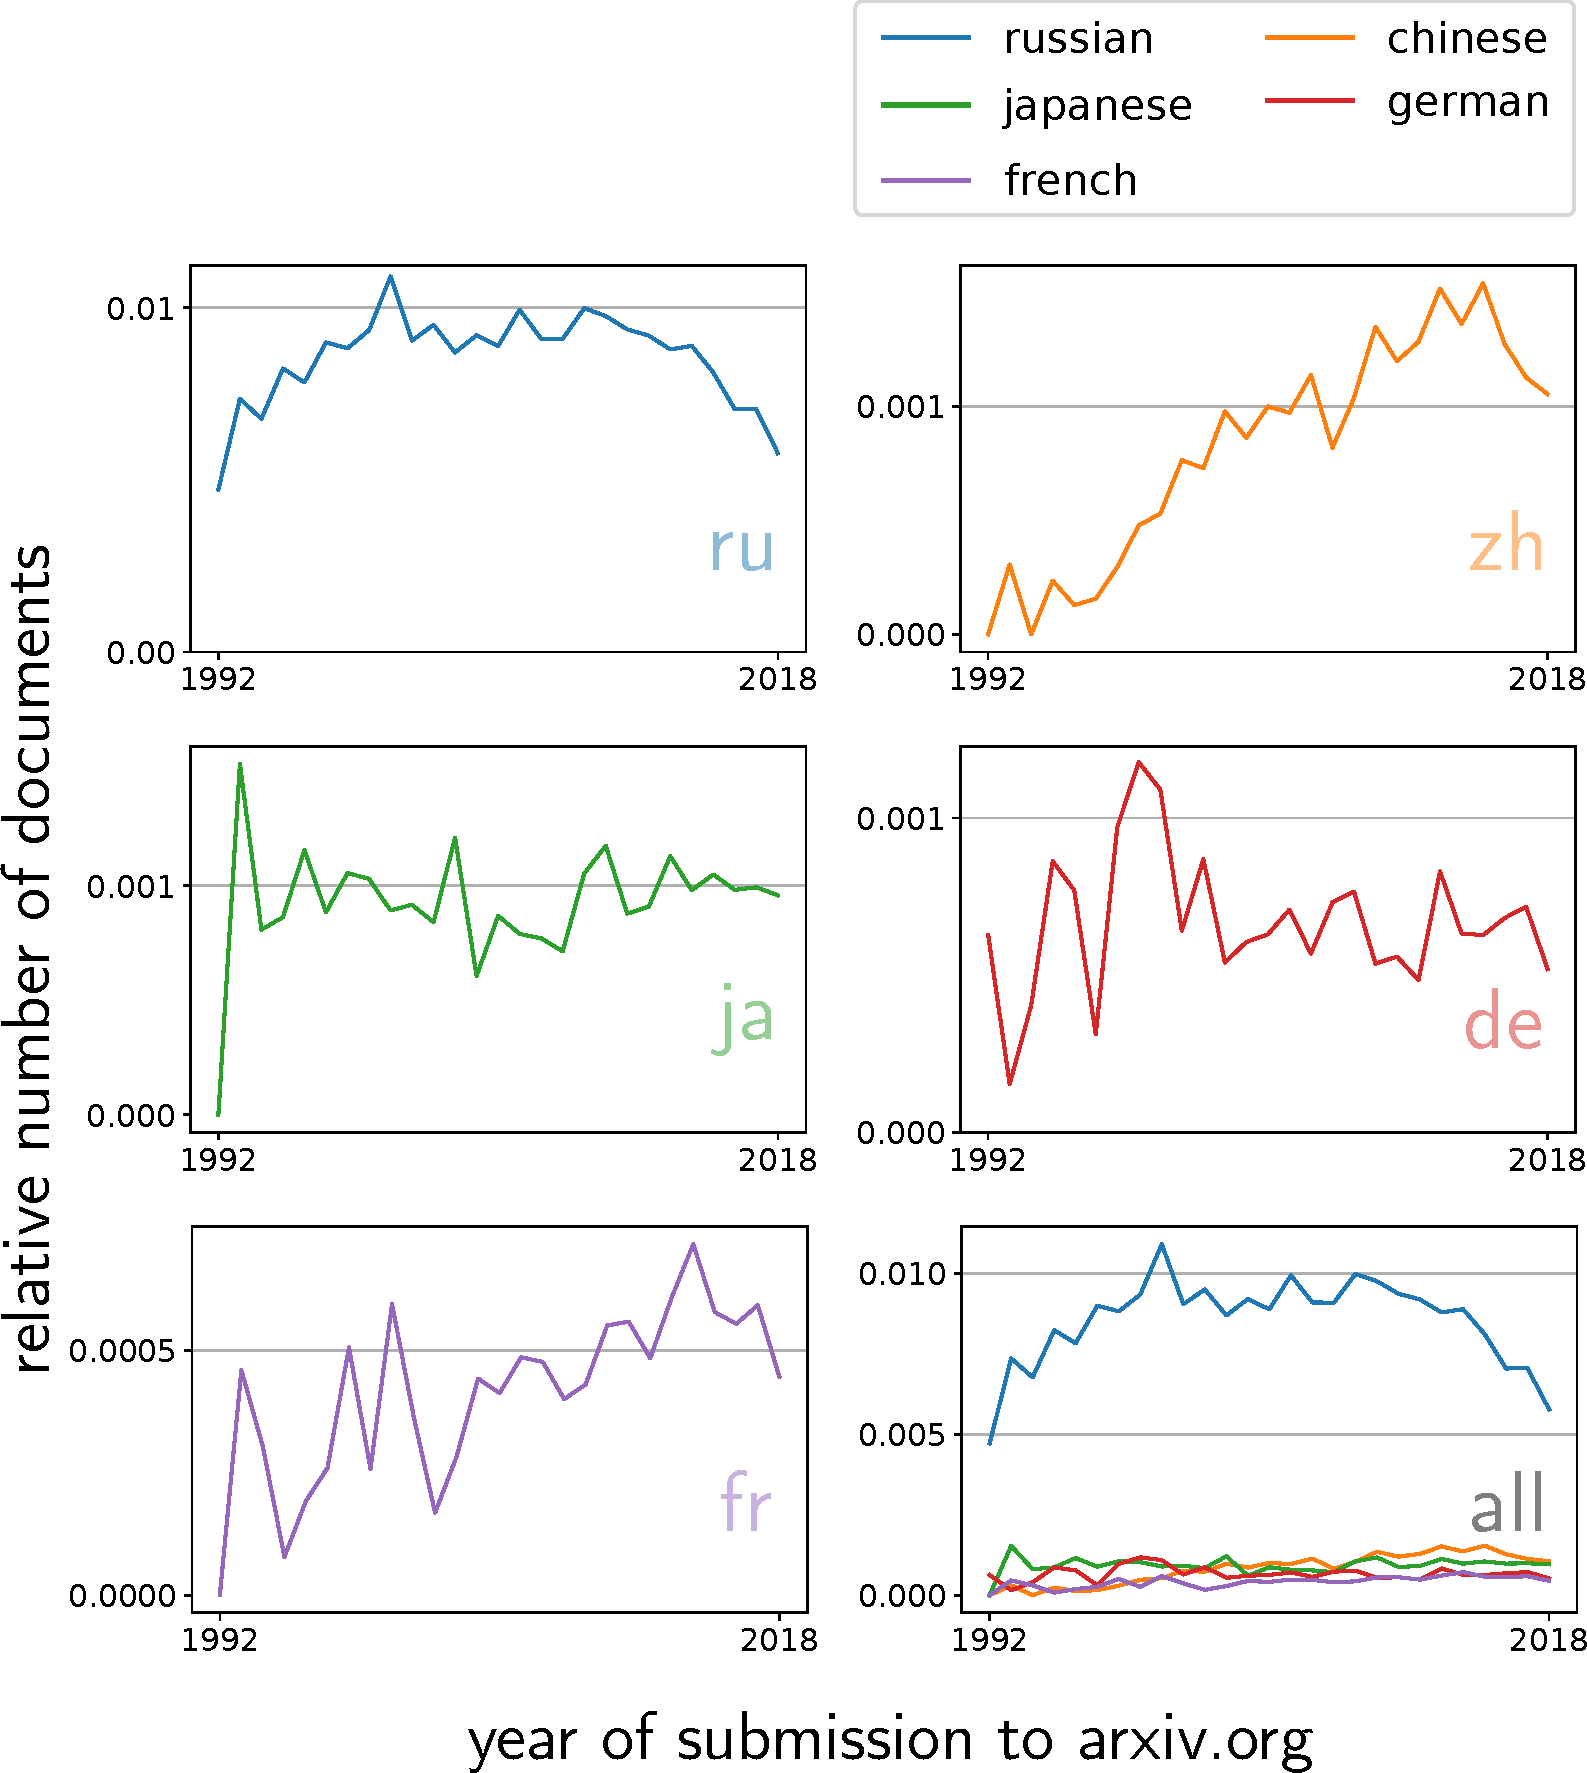
\includegraphics[width=0.7\linewidth]{figures/ref_xling/relative_language_counts_across_time_mod_twocolumn.pdf}
\caption[Relative number of documents citing Russian, Chinese, Japanese, German, and French works]{Relative number of documents citing Russian, Chinese, Japanese, German, and French works. Showing all aforementioned in the bottom right.} \label{fig:previntime}
\end{figure}

\begin{figure}[tb]
\centering
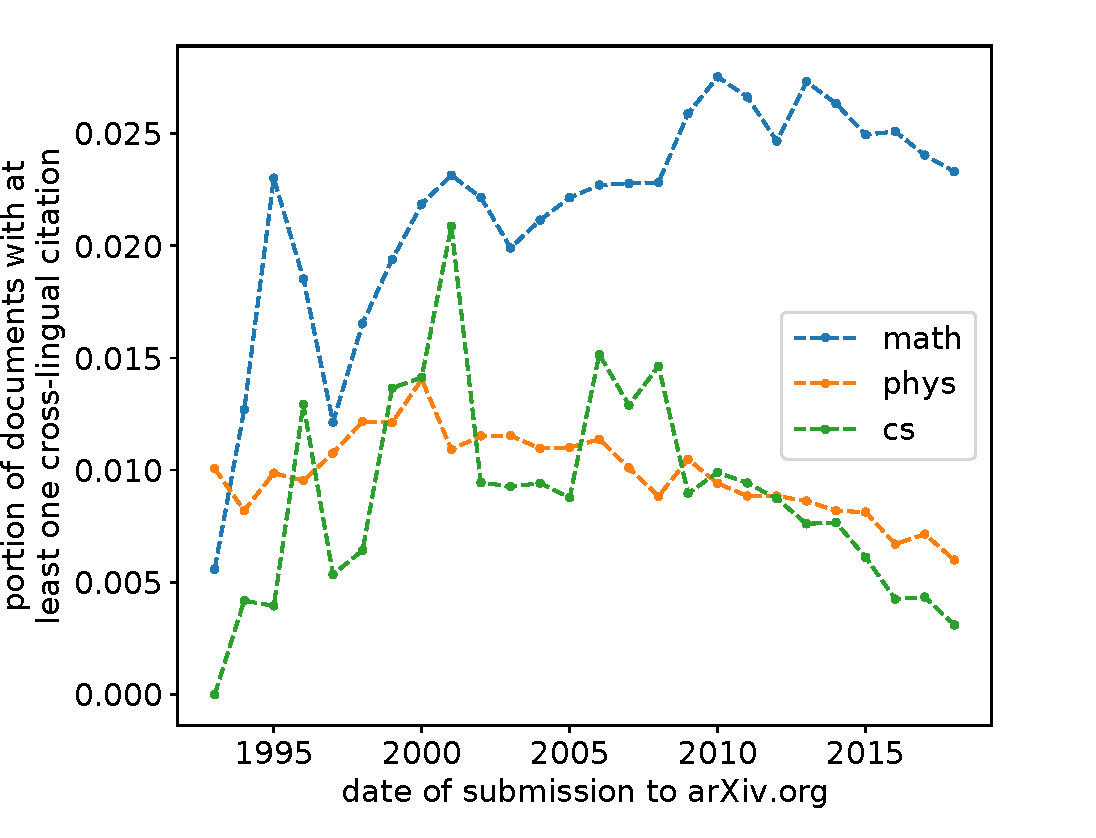
\includegraphics[width=0.7\linewidth]{figures/ref_xling/relative_number_of_papers_lessthan64.pdf}
\caption{Relative number of mathematics, physics, and computer science documents citing non-English works.} \label{fig:prevperdisc}
\end{figure}

\begin{figure}[tb]
\centering
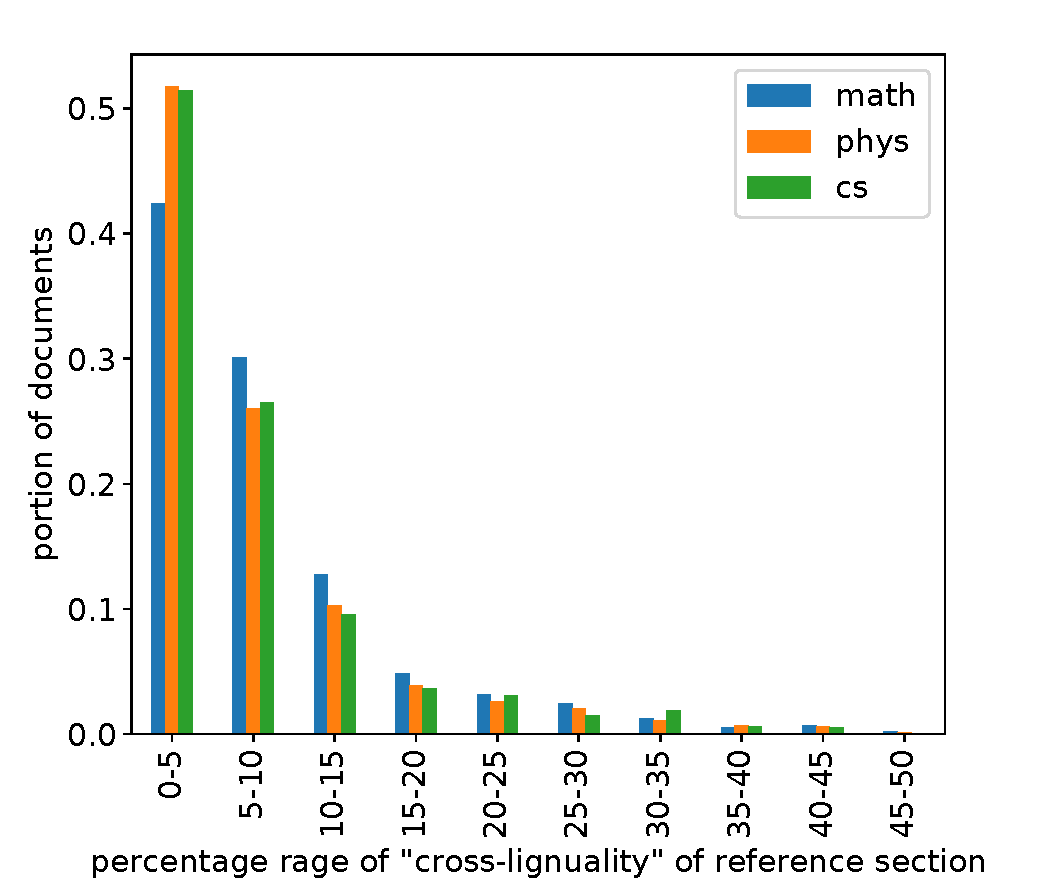
\includegraphics[width=0.7\linewidth]{figures/ref_xling/cross_ling_ratio_distribution_lessthan64.pdf}
\caption{``Cross-linguality'' of reference sections by discipline.} \label{fig:xlinglyhistbydisc}
\end{figure}

Lastly, within the reference section of a document that has at least one cross-lingual citation, the mean value of ``cross-linguality'' (i.e., what portion of the reference section is cross-lingual) is 0.083 with a standard deviation of 0.099. Breaking these numbers down by discipline, we can see in Figure~\ref{fig:xlinglyhistbydisc} that there is no large difference, although mathematics papers tend to have a slightly higher portion of cross-lingual citations. The mean values for mathematics, physics and computer science are 0.090, 0.078, and 0.080 respectively.

Regarding prevalence we observe that in English papers in the disciplines of physics, mathematics, and computer science about 1 in 66 publications contains at least one explicitly marked citation to a non-English document. About two thirds of these citations are to Russian documents, although in the last years there is a downwards trend with regard to Russian and an upwards trend in citations to Chinese. Furthermore, cross-lingual citations appear about twice as often in mathematics compared to physics and computer science.
These observations suggest that while cross-lingual citations are not very frequent in general, they might be worth considering in applications dealing with specific disciplines and languages (e.g. citations to Russian in mathematics publications).

\subsection{Usage}

Regarding the usage of cross-lingual citations in English publications we analyze four different aspects. (1)~Whether or not self-citations are a driving factor, (2)~to what degree the geographical origin of a cross-lingual citation is correlated with the cited document's language, (3)~what function they serve, and (4)~what sentiment they express toward the cited document.

\subsubsection{Self-citation}\label{sec:selfcit}

To assess the relative degree of self-citation when referring to publications in other languages, we compare the ratio of self-citations in (a)~the \emph{cross-lingual citations} within the documents of the cross-lingual set, and (b)~the \emph{monolingual citations} within the documents of the cross-lingual set. Comparing two sets of citations from identical documents allows us to control for confounding effects such as author specific self-citation bias.

To determine self-citation, we rely on the author metadata in the MAG and therefore require both the citing and cited document of a reference to have a MAG ID. Within the cross-lingual set, this is the case for 3,370 cross-lingual references and 264,341 monolingual references. While at first, we strictly determine a self-citation by author IDs in the MAG being identical, manual inspection of matches and non-matches reveals, that author disambiguation within the MAG is somewhat lacking---that is, in a non-trivial amount of cases there are several IDs for a single author. We therefore measure self-citation by two metrics. A strict metric which only counts a match of MAG IDs, and a loose metric which counts an overlap of the sets of author names on both ends of the reference as a self-citation.

\begin{table}[tb]
\caption{Self-citations}
 \label{tab:selfcit}
  \centering
  \begin{small}
 \begin{threeparttable}
 \begin{tabular}{lrr}
 \toprule
   \ & \multicolumn{2}{c}{Self-citations} \\
   References to & loose & strict \\
   \midrule
   non-English & 19\% & 5\% \\
   English & 17.9\% & 11.3\% \\
   \bottomrule
 \end{tabular}
\end{threeparttable}
  \end{small}
\end{table}

Table~\ref{tab:selfcit} shows that going by the strict metric, self-citation is twice as common in monolingual citations. Applying the loose metric, however, self-citation appears to be slightly more common in cross-lingual citations. The larger discrepancy between the results of the strict and loose metric for cross-lingual citations suggests that authors publishing in multiple languages might be less well disambiguated in the MAG. With regard to self-citation being a motivating factor for cross-lingual citations---be it, for example, due to the need to reference one's own prior work---, we can note that our data does not suggest this to be the case. Authors using cross-lingual citations appear to be at least equally as likely to self-cite when referencing English works.

\subsubsection{Geographical Origin}

\begin{figure}[tb]
\centering
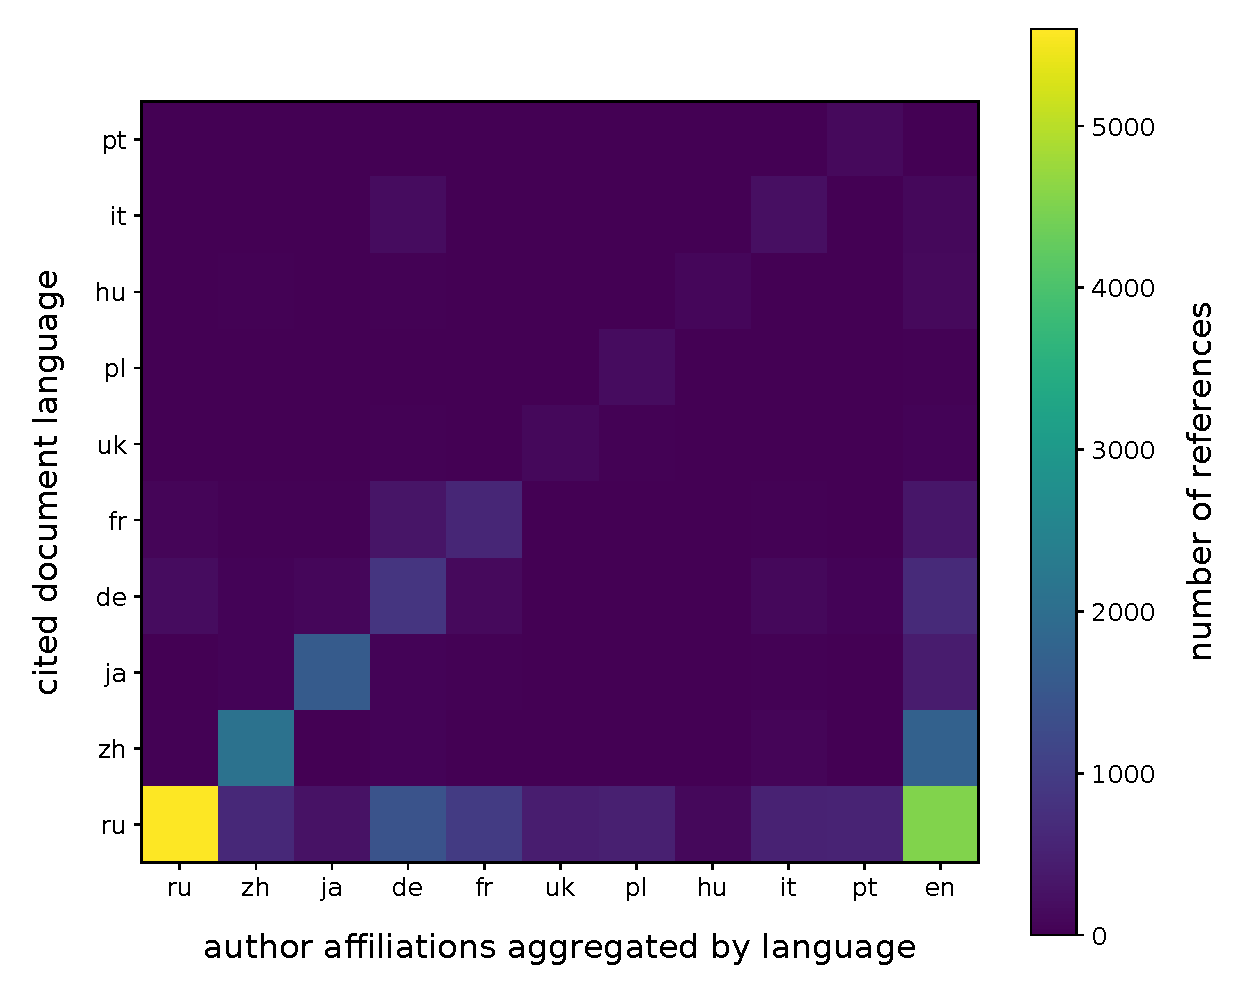
\includegraphics[width=0.7\linewidth]{figures/ref_xling/citlang_to_author_aff_absolute_crop.pdf}
\caption{Geographic origin of cross-lingual citations to the ten most cited languages (absolute count).} \label{fig:geo_abs}
%\end{figure}

%\begin{figure}[tb]
\centering
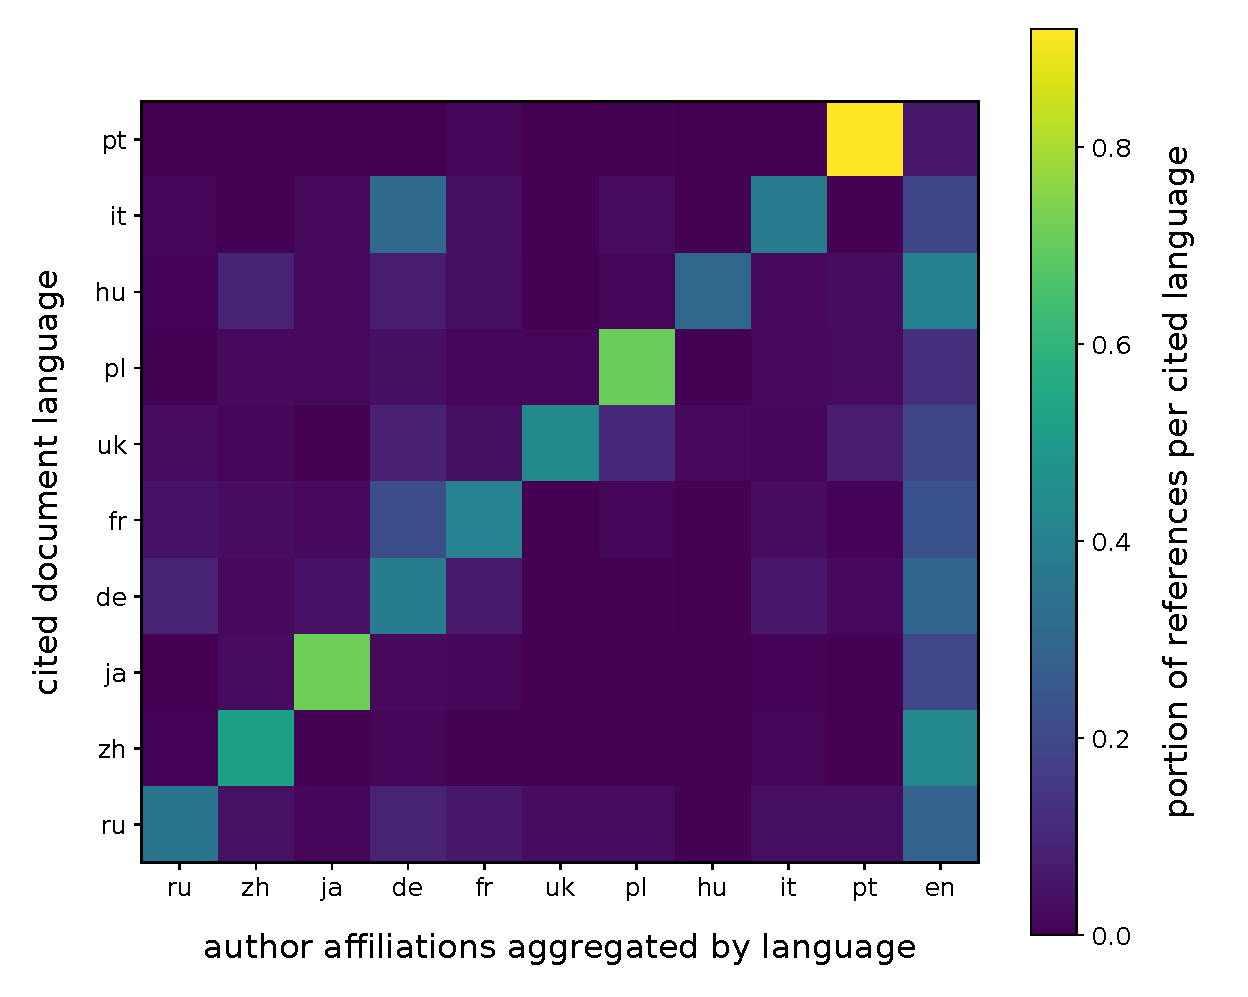
\includegraphics[width=0.7\linewidth]{figures/ref_xling/citlang_to_author_aff_relative_crop.pdf}
\caption{Geographic origin of cross-lingual citations to the ten most cited languages (relative count).} \label{fig:geo_rel}
\end{figure}

In this section we analyze the geographical origin of cross-lingual citations. As a measure for geographical origin we use the country in which a citing author's affiliation is located. We refer to a citation as being to a ``local language'' or of ``local origin'', if the cited document's language is the most commonly spoken language in the affiliation's location. An example of this would be a researcher affiliated with a research institution located in Russia, being the author of a paper in which they cite a publication written in Russian.

For our analysis, we rely on author affiliation metadata in the MAG. We start off with all documents in the cross-lingual set that have a MAG ID.\footnote{I.e., documents for which we have MAG metadata (see Table~\ref{tab:dataused}).} From those, we select all which provide information on the authors' affiliations.\footnote{Because a single paper can have authors affiliated with institutions in different locations, we perform our analysis on a per author basis.} This leaves us with 7,522 out of 16,300 papers. To associate an author's affiliation with a language, we use the most commonly spoken language in the country or territory.\footnote{The association between affiliation and country is already given in the MAG. For data on language use per country we refer to the Unicode Common Locale Data Repository's territory-language information (see \url{https://unicode-org.github.io/cldr-staging/charts/latest/supplemental/territory_language_information.html}).} Grouping affiliations by language, we can then view the correlation of (a) cited languages and (b) language grouped affiliations in two ways. On the one hand, we can see for each cited language how many of the citations are of local origin---compared to, for example, from an English speaking country. On the other hand, we can see for each language group of affiliations how many cross-lingual citations are to a local language. Our results of this analysis are shown for the 10 most commonly cited languages in Figures~\ref{fig:geo_abs} and~\ref{fig:geo_rel}, and for all identified cited languages in Appendix~\ref{sec:apndx_geo}.

Figure~\ref{fig:geo_abs} shows citation numbers in absolute terms. Looking, for example, at citations to Russian publications (the bottom row of the figure), we can see that the largest amount of citations originates from Russian speaking countries (5,599 out of 18,672) followed by English speaking countries (4,535) and German speaking countries (1,427).

In Figure~\ref{fig:geo_rel} we show relative numbers per cited language. That is, the values of each \emph{row} add up to 1. Here we can see that citations to Japanese, Polish and particularly Portuguese appear to be of local origin comparatively often, with 68\% for Japanese, 64\% for Polish and 86\% for Portuguese. Overall we observe that cross-lingual citations are most often either of local origin or from an English speaking country. Evaluated over all languages, 37\% of cross-lingual citations are local (the diagonal in Figures~\ref{fig:geo_abs} and~\ref{fig:geo_rel}), while 26\% are from the Anglosphere (the ``en'' column in Figures~\ref{fig:geo_abs} and~\ref{fig:geo_rel}).

\begin{figure}[tb]
\centering
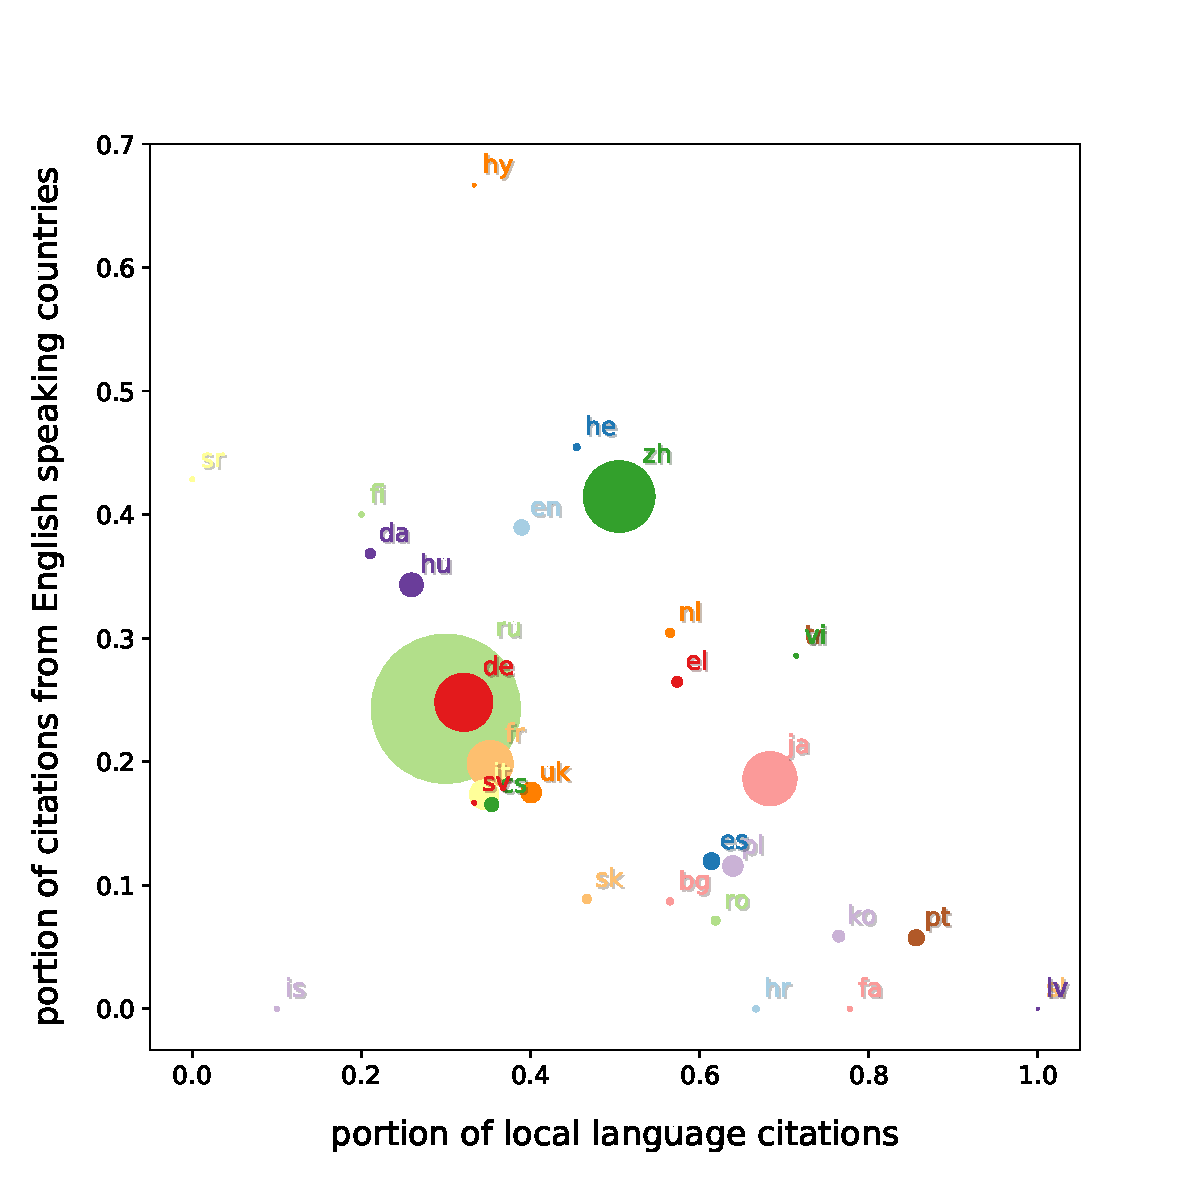
\includegraphics[width=0.7\linewidth]{figures/ref_xling/citation_origin_local_vs_en.pdf}
\caption[Geographic origin of cross-lingual citations (local vs. English speaking countries)]{Geographic origin of cross-lingual citations (local vs. English speaking countries). Marker size (surface area) indicates number of citations.} \label{fig:geo_localvsen}
\end{figure}

In Figure~\ref{fig:geo_localvsen} we jointly visualize how ``locally'' cited each language in our corpus is (x-axis) compared to which portion of citations originate from English speaking countries (y-axis). Overall, we observe larger variation on the ``locality'' dimension (values ranging from 0 to 1 with a variance of 0.058) than on the ``from English speaking countries'' dimension (values from 0 to 0.67 with a variance of 0.026). Looking at non-Latin script languages, we can see that Cyrillic script languages (e.g., Russian and Ukrainian) are less often of local origin than Asian languages (Chinese, Japanese, Korean) or languages written in Arabic script (Persian\footnote{While most varieties of Persian are written in a version of the Arabic script, there also exists varieties written in Cyrillic script~\cite{Megerdoomian2008}.}). Narrowing down on above-mentioned three Asian languages, we observe that for Chinese the relative portion of citations from English-speaking countries (0.41) is more than double of the same measure for Japanese (0.19), which is more than triple the value for Korean (0.06). The comparatively high ratio for Chinese (not just among Asian languages but overall\footnote{The overall comparison has, however, to be done keeping the limitations described in Section~\ref{sec:ident} in mind.}) could be taken as an indication for two phenomena: first, an increased relevance of publications written in Chinese (i.e., a higher necessity to cite) and second, an increased rate of scholars able to read Chinese in English speaking country research institutions (i.e., a higher probability of the ability to cite).

\subsubsection{Citation Intent and Sentiment}

To assess whether or not cross-lingual citations tend to serve a different purpose than their monolingual counterpart, and whether or not authors have a different disposition toward cited works, we analyze the in-text citations (see Figure~\ref{fig:terminology}) in our corpus.

The analysis of in-text citations---commonly referred to as citation context analysis---is concerned with the textual context of citations~\cite{Hernandez2016}. Two tasks in citation context analysis are the classification of citation intent (also referred to as citation function) and citation sentiment (also referred to as citation polarity)~\cite{Hernandez2016}. Citation intent can reveal why an author added a reference, while the citation sentiment can give insight into the author's disposition toward that reference. Both citation intent and sentiment have been used in a number of diverse tasks, such as classification \cite{Jurgens2018,Cohan2019,Beltagy2019}, summarization \cite{Cohan2015}, and citation recommendation \cite{Faerber202x}. For citation intent, many schemes have been proposed to classify different functions, ranging from fine-grained to coarse-grained schemes. A partial overview of these can be found in Hernández-Alvarez~\cite{Hernandez2016}, Jurgens et al.~\cite{Jurgens2018}, Cohan et al.~\cite{Cohan2019}, and Lauscher et al.~\cite{multicite-lauscher-2021}. These schemes, however, are often domain-specific and too fine-grained~\cite{Cohan2019}. Jurgens et al.~\cite{Jurgens2018} proposed a unified scheme of previous work (with six categories), while Cohan et al.~\cite{Cohan2019} proposed a more generalized scheme (with three categories) that works for multiple domains. Recently, Lauscher et al. ~\cite{multicite-lauscher-2021} expanded these schemes to multi-sentence and multi-label citation contexts. Given the number of diverse domains on arXive, we adopt the general scheme by Cohan et al.~\cite{Cohan2019}. For citation sentiment, a three category scheme (\textit{positive}, \textit{negative}, or \textit{neutral}) is widely adopted~\cite{Athar2011,Abujbara2013,Hernandez2016}. Previous approaches to citation intent and sentiment classification have used either hand-crafted rules or classical machine learning models~\cite{Abujbara2013,Jurgens2018}, while more recent approaches using deep learning and word embeddings have demonstrated significant improvements in performance~\cite{Cohan2019,Beltagy2019,multicite-lauscher-2021}.

For our analysis, we create two, equally-sized sets of in-text citations. The \textit{in-text x-ling} set (cross-lingual) and the \textit{in-text mono} set (monolingual). In the following we describe the creation of both sets, the classifier model training, and our results for citation intent and sentiment classification.

\textsc{Data Preparation}
For the \textit{in-text x-ling} set we determine all in-text citations associated with the references in the cross-lingual set. This yields 45,516 in-text citations for our 33,290 cross-lingual references. The \textit{in-text mono} set is then created by extracting in-text citations associated with adjacent monolingual references. We illustrate this process in Figure~\ref{fig:adjrefsampling}, showing a paper with a single cross-lingual reference for which, accordingly, a single adjacent monolingual reference would be determined and its associated in-text citations (indicated by the two blue markers above) extracted. For \textit{in-text mono} we extract 53,177 in-text citations (i.e., on average more in-text citations per reference) which we reduce to 45,516 through stratified sampling. By sourcing our monolingual in-text citations for comparison from the same papers, we avoid confounding effects such as author specific differences in citation styles.

\begin{figure}[tb]
\centering
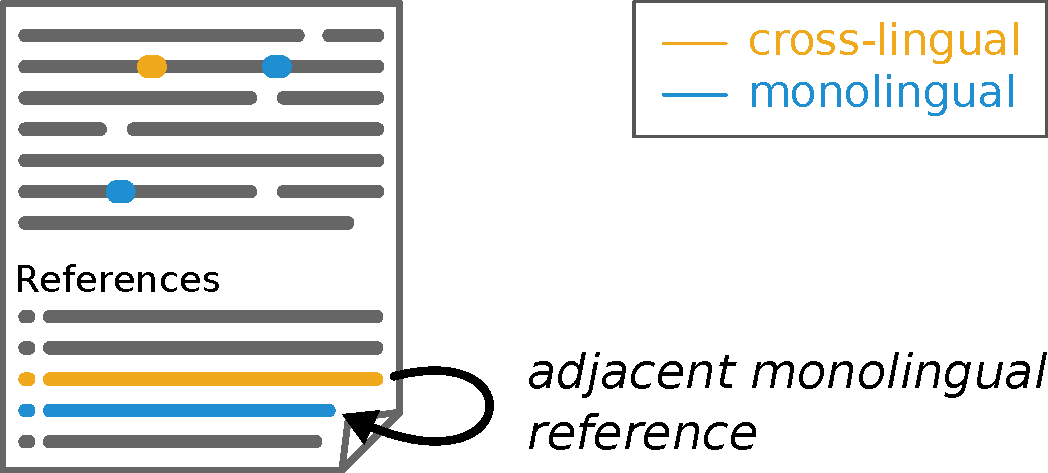
\includegraphics[width=0.5\linewidth]{figures/ref_xling/adjacent_reference_sampling.pdf}
\caption{Schematic explanation of an adjacent monolingual reference.} \label{fig:adjrefsampling}
\end{figure}

As a citing sentence can contain more than one citation marker, it is possible that the in-text citations associated with two adjacent reference section entries appear within the same sentence (e.g., as indicated in the second ``text'' line in Figure~\ref{fig:adjrefsampling}). This is the case for 10,454 of the in-text citations we extracted (i.e., these appear in both sets). We define them as a third set called \textit{mixed}, leaving \textit{in-text x-ling} and \textit{in-text mono} at 35,062 items each.

\begin{table}
\caption{Class distribution and evaluation details for the model training.}
 \label{tab:classdist}
  \centering
  \begin{small}
 \begin{threeparttable}
 \begin{tabular}{lrrrrrr}
 \toprule
   Data set & Class & Inst.\tnote{a}\hphantom{\,} & Precision & Recall & F1-macro \\
   \midrule
   \multirow{3}{*}{SciCite} & Backgr. & 6,375 (58) & 86\% & 93\% & \multirow{3}{*}{86.6\%}\\
                            & Method & 3,154 (29) & 91\% & 82\%\\
                            & Result & 1,491 (13) & 86\% & 83\% \\ \midrule\midrule
  \multirow{3}{*}{Athar} & Neutral & 6,901 (87) & 91\% & 98\% & \multirow{3}{*}{67.9\%} \\
                          & Positive & 761 (10) & \textbf{80\%} & 42\% \\
                          & Negative & 265 (3) & 50\% & 29\% \\ \midrule
  \multirow{3}{*}{Athar$^{\dagger}$} & Neutral & 265 (33) & 77\% & 59\% & \multirow{3}{*}{67.7\%} \\
                          & Positive & 265 (33) & 59\% & 59\% \\
                          & Negative & 265 (33) & \textbf{65\%} & \textbf{94\%} \\ \midrule
    \multirow{2}{*}{Athar$^{\mathsection}$} & Neutral & 6,901 (90) & \textbf{96\%} & \textbf{97\%} & \multirow{2}{*}{82.5\%} \\
                            & Positive & 761 (10) & 69\% & 68\% \\ \midrule
    \multirow{2}{*}{Athar$^{\ddagger}$} & Neutral & 761 (50) & 85\% & 69\% & \multirow{2}{*}{80.2\%} \\
                            & Positive & 761 (50) & 78\% & \textbf{90\%} \\
   \bottomrule
 \end{tabular}
 \begin{tablenotes}
    \item[a] Inst. = Number of instances for training and evaluation (percentage in brackets)
    \item $^{\dagger}$ = Under-sampled
    \item $^{\mathsection}$ = No \textit{Negative} class
    \item $^{\ddagger}$ = Under-sampled \& no \textit{Negative} class
 \end{tablenotes}
\end{threeparttable}
  \end{small}
\end{table}

\textsc{Model Training}
Training data for citation sentiment and intent classification regarding papers cannot easily be crowdsourced, because domain knowledge is needed for annotation. As a consequence, available data sets are comparatively small. We identify SciCite~\cite{Cohan2019} for citation intent and the data set proposed by Athar~\cite{Athar2011} for citation sentiment as most appropriate for our purposes.

\begin{itemize}
\item SciCite contains 11,020 citations that originate from the Semantic Scholar corpus, which covers several disciplines such as computer science, molecular biology, microbiology and neuroscience~\cite{Ammar2018}. Citations in SciCite are labeled regarding their intent across three categories, namely \textit{Background}, \textit{Method}, and \textit{Result}. The class distribution can be seen in Table \ref{tab:classdist}. We select the data set because it is currently the largest available, and classifiers trained on the data set achieve good performance.

\item The data set created by Athar contains 8,736 annotated citations from 310 research papers. To the best of our knowledge, it is the largest citation sentiment data set currently available. Following~\cite{Mercier2021}, we manually remove 809 items from the data set that are either duplicates or too short to be accurately evaluated regarding their sentiment. The resulting data set, which we refer to as \textit{Athar} from hereon, contains 7,927 citations annotated with one of the three labels \textit{Negative}, \textit{Neutral}, and \textit{Positive}. Citations labeled \textit{Negative} and \textit{Positive} are comparably infrequent in the corpus (see Table \ref{tab:classdist}), which makes classifying them more difficult. As possible mitigation strategies, we consider the following options.
    \begin{itemize}
    \item Athar$^{\dagger}$: balancing the data by under-sampling.
    \item Athar$^{\mathsection}$: removing the \textit{Negative} class, as its low performance (see Table~\ref{tab:classdist}) puts its informativeness into question.
    \item Athar$^{\ddagger}$: both of the aforementioned.
    \end{itemize}
\end{itemize}

For each of our classification models, we fine-tune SciBERT~\cite{Beltagy2019}, a pre-trained language model for scientific text that achieves state-of-the-art performance on sentence classification tasks.

Our evaluation results are shown in Table~\ref{tab:classdist}. On both SciCite and Athar our models perform on par with the best performing models presented in their respective publications. For citation intent, we achieve an F1 score of 86.6\% and relatively similar performance across classes. For citation sentiment, we achieve an F1 score of 67.9\% on the original Athar data set. Two of our three class imbalance mitigation strategies (Athar$^{\mathsection}$ and Athar$^{\ddagger}$) result in an increase in the F1 score to over 80\%. Of those two we decide to use the model trained on Athar$^{\ddagger}$. While training on Athar$^{\mathsection}$ gives us a slightly higher F1 score, the model trained on Athar$^{\ddagger}$ achieves high precision and recall for positive citations---which are presumably less common---while also maintaining good performance for neural citations.
Implementation details for the model training can be found in Ap\-pen\-dix~\ref{app:classifcation}.

\begin{table}[tb]
\caption[Citation intent and sentiment classification results for cross-lingual, monolingual, and mixed in-text citations]{Citation intent and sentiment classification results for cross-lingual, monolingual, and mixed in-text citations. (Values are the number of citations per class followed by the percentage in brackets.)}
 \label{tab:citationclassificationdist}
  \centering
  \begin{small}
 \begin{threeparttable}
 \begin{tabular}{lrrr}
 \toprule
  Data set\hphantom{\ } & Background\hphantom{\ } & Method\hphantom{\ } & Result\hphantom{\ }\\
  \midrule
    \textit{x-ling} & 26,443 (75.4) & 7,749 (22.1) & 870 (2.5) \\
    \textit{mono} & 26,232 (74.8) & 7,801 (22.2) & 1,029 (2.9) \\
    %\midrule
    \textit{mixed} & 7,688 (73.5) & 2,503 (23.9) & 263 (2.5) \\
  \midrule
  \midrule
  & Neutral\hphantom{\ } & Positive\hphantom{\ } & Negative\hphantom{\ }\\
  \midrule
    \textit{x-ling*} & 34,100 (97.3) & 787 (2.2) & 175 (0.5) \\
    \textit{mono*} & 33,792 (96.4) & 1,037 (3.0) & 233 (0.7) \\
    \textit{mixed*} & 10,049 (96.1) & 362 (3.5) & 43 (0.4) \\ \midrule
    \textit{x-ling$^{\ddagger}$} & 22,275 (63.5) & 12,787 (36.5) & \\
    \textit{mono$^{\ddagger}$} & 21,825 (62.3) & 13,237 (37.8) & \\
    \textit{mixed$^{\ddagger}$} & 6,547 (62.6) & 3,907 (37.4) & \\
  \bottomrule
 \end{tabular}
  \begin{tablenotes}
    \item * = Classified using the model trained on Athar
    \item $^{\ddagger}$ = Classified using the model trained on Athar$^{\ddagger}$
    % \item*** = Unbalanced 
 \end{tablenotes}
\end{threeparttable}
  \end{small}
\end{table}

\begin{figure}[tb]
\centering
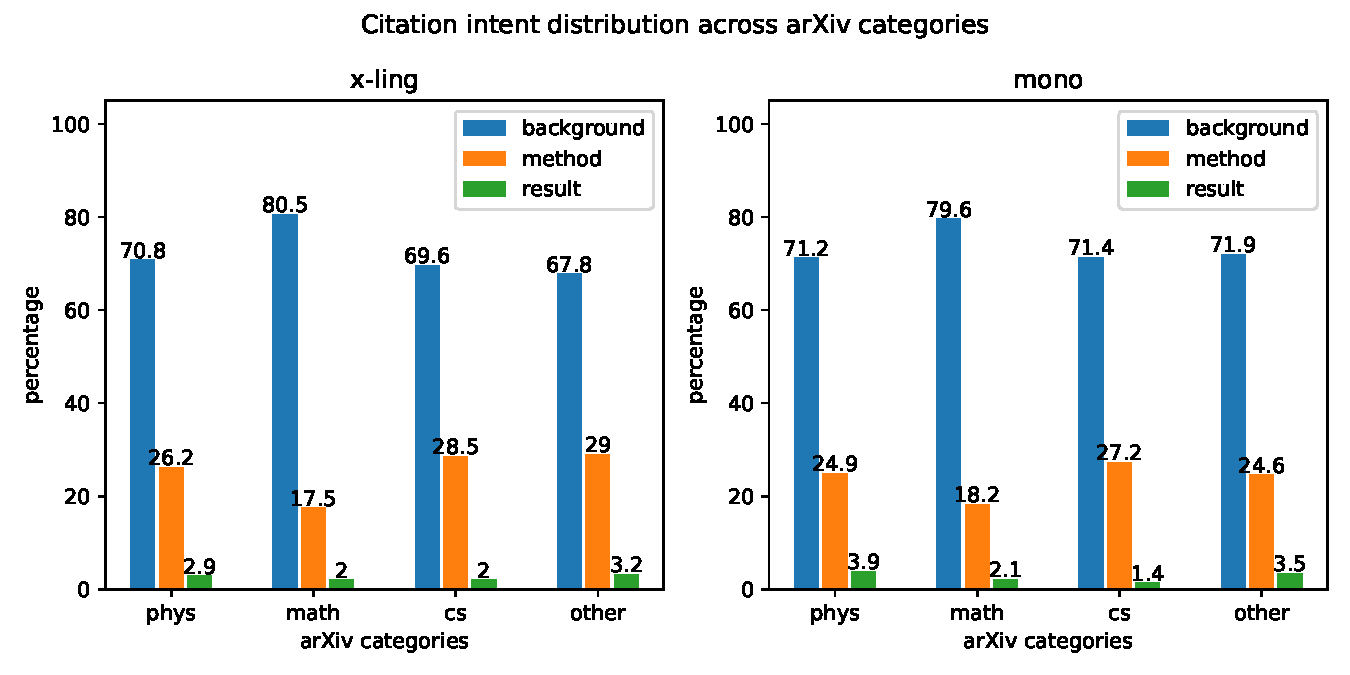
\includegraphics[width=\linewidth]{figures/ref_xling/cross_ling_citation_intent_arxive_categories.pdf}
\caption[Comparison of citation intent distribution across arXiv categories for \textit{in-text x-ling} and \textit{in-text mono}]{Comparison of citation intent distribution across arXiv categories for \textit{in-text x-ling} (left) and \textit{in-text mono} (right).} \label{fig:intentarxivcategories}
\end{figure}

\textsc{Classification Results}
Based on above evaluation we proceed by using our models trained on SciCite, Athar, and Athar$^{\ddagger}$ to classify the intent and sentiment of citations in \textit{in-text x-ling} and \textit{in-text mono}.
In Table~\ref{tab:citationclassificationdist}, we show the classification results for citation intent (top half) and sentiment (bottom half). The classifiers trained on SciCite and Athar appear to amplify the unbalanced data distribution they were trained on to some degree. Comparing the sentiment classifiers trained on the original Athar and balanced Athar$^{\ddagger}$ data set, we see that citations classified as \textit{Positive} increase from around 3\% to almost 38\%. We take this as a clear sign that reliably distinguishing neutral from positive citations remains a challenge even with state-of-the art models and training data.

Comparing our results across the data sets \textit{in-text x-ling}, \textit{in-text mono}, and \textit{in-text mixed} we see that in terms of both intent and sentiment class distributions are similar. Taking a closer look at citation intent across the scientific disciplines,\footnote{We do not evaluate citation sentiment here due to the lacking performance of the sentiment classifiers.} we can see in Figure~\ref{fig:intentarxivcategories} that the distributions are overall comparable among disciplines and between cross- and monolingual citations, with mathematics showing a slightly higher use of background citations.


Overall, our results for citation sentiment and intent show no distinct differences between cross- and monolingual citations. This can be taken as an indication for two things. First, that authors cite existing literature with a certain intent and sentiment \emph{regardless} of the cited work's language. Second, that cross-lingual---while occurring less frequent---serve the same functions as monolingual citations and are therefore not less significant.


\subsection{Impact}
Regarding the impact of cross-lingual citations we analyze whether cross-lingual citations in English papers are seen as an ``acceptable'' practice, whether or not they pose a particular challenge for citation data mining, and their potential impact on the success of the paper they're part of. Our results concerning these three aspects are described in the following sections.

\subsubsection{Acceptance}

To assess the acceptance of cross-lingual citations by the scientific community---that is, whether or not non-English publications are deemed ``citable''~\cite{Lillis2010}---we analyze papers in our data that have both a preprint version as well as a published version (in a journal or conference proceedings) dated later than the preprint. This is the case for 2,982 papers. For each preprint-published paper pair, we check if there is a difference in cross-lingual citations. This gives an indication of how the process of peer review affects cross-lingual citations.
We perform a manual as well as an automated analysis.\footnote{Full evaluation details can be found at \url{https://github.com/IllDepence/cross-lingual-citations-from-en}.}

For the manual evaluation, we take a random sample of 100 paper pairs. We then retrieve a PDF file of both the preprint and the published version, and manually compare their reference sections. For the automated evaluation, we find that 599 of the 2.9k paper pairs have PDF source URLs given in the MAG. After automatically downloading these and parsing them with GROBID, we are left with 498 valid sets of references. For these, we identify explicitly marked cross-lingual references as described in Section~\ref{sec:datacollection} and calculate their differences.

Table~\ref{tab:peerreview} shows the results of our evaluations. In both, cross-lingual citations are more often removed than added, but in the majority of cases left intact. The larger volatility in the automated evaluation is likely due to parsing inconsistencies of GROBID. Our findings complement those of Lillis et al.~\cite{Lillis2010}, who, analyzing psychology journals, observe \textit{``some evidence that gatekeepers [...] are explicitly challenging citations in other languages.''} For the fields of physics, mathematics, and computer science, we find no clear indication of a consistent in- or decreasing effect of the peer review process on cross-lingual citations.

\begin{table}
\caption{Changes in cross-ling. cit. between preprints and published papers}
 \label{tab:peerreview}
  \centering
  \begin{small}
 \begin{threeparttable}
 \begin{tabular}{lrrrrrr}
 \toprule
   Evaluation & \#Pairs & \#Inc.\tnote{a} & \#Dec.\tnote{b} & Mean\tnote{c} & SD\tnote{c} \\
   \midrule
   Manual & 100 & 4 & 7 & -0.02 & 0.529 \\
   Automated & 498 & 33 & 70 & -0.12 & 0.821 \\
   \bottomrule
 \end{tabular}
 \begin{tablenotes}
    \item[a] Inc. = Increased
    \item[b] Dec. = Decreased
    \item[c] of the differences in the amount of cross-lingual citations
 \end{tablenotes}
\end{threeparttable}
  \end{small}
\end{table}

\subsubsection{Impact on Paper Success}

To get an indication of whether or not an English paper's success is influenced by the fact that it contains citations to non-English documents, we compare our cross-lingual set with the random set (cf. Table~\ref{tab:datasets}). For both sets we first determine the number of papers that in the MAG metadata have a published version (journal or conference proceedings) in addition to the preprint on arxiv.org. That is, we assume that papers which only have a preprint version did not make it through the peer review process. Using this measure, we observe 9,390 of 16,224 (57.88\%) successful papers in the cross-lingual set, and 10,966 of 16,378 (66.96\%) successful papers in the random set. Unsurprisingly, due to the higher ratio of published versions, the papers in the random set are also cited more. Table~\ref{tab:citcounts} shows a comparison of the average number of citations that documents in both sets received. Due to the high standard deviation in the complete sets, we also look at papers which received between 1 and 100 citations, which are comparably frequent in both sets. As we can see, in the unfiltered as well as the filtered case, documents with cross-lingual citations tend to be cited a little less. Because here we can only control for the distribution of papers across years and disciplines, and not for individual authors (as we did in the Section~\ref{sec:selfcit}), there might be various confounding factors involved.


\begin{table}[tb]
\caption{Comparison of citations received}
 \label{tab:citcounts}
  \centering
  \begin{small}
 \begin{threeparttable}
 \begin{tabular}{llrr}
 \toprule
   \multicolumn{2}{l}{Filter criterion} & Cross-lingual set & Random set \\
   \midrule
   - & \#Docs & 16,300 & 16,464 \\
   \ & Mean \#cit & 13.7 & 18.2 \\
   \ & SD & 75.0 & 51.7 \\
   \midrule
   $1\le \#cit$ & \#Docs & 12,074 & 12,852 \\
   and & Mean \#cit & 12.0 & 15.1 \\
   $\#cit\le 100$ & SD & 15.8 & 18.4 \\
   \bottomrule
 \end{tabular}
\end{threeparttable}
  \end{small}
\end{table}

\subsubsection{Impact on Citation Data Mining}

To assess if cross-lingual citations pose a particular challenge for scholarly data mining---and are therefore likely to be underrepresented in scholarly data---, we compare the ratio of references that could be resolved to MAG metadata records for the cross-lingual set and the whole unarXive data set. Of the 39M references in unarXive 42.6\% are resolved to a MAG ID. For the complete reference sections of the papers in the cross-lingual set (i.e., references to both non-English and English documents) the number is 45.7\% (290,421 of 635,154 references). Looking only at the cross-lingual citations, the success rate of reference resolution drops to 11.2\% (3,734 of 33,290 references). We interpret this as a clear indication that resolving cross-lingual references is a challenge. Possible reasons for this are, for example:
\begin{enumerate}
\item A lack of language coverage in the target data set.\\For example, if the target data set only contains records of English papers, references to non-English publications cannot be found within and resolved to that target data set.
\item Missing metadata in the target data set.\\For example, when there is a primary non-English as well as an alternative English title of a publication, only the former is in the target data set's metadata, but the latter is used in the cross-lingual reference.
\item The use of a title translated ``on the fly.''\\If a non-English publication has no alternative English title, a self translated title in a reference cannot be found in any metadata. To give an example, reference 14 in \texttt{arXiv:1309.1264} titled \textit{``Hierarchy of reversible logic elements with memory''} is only found in metadata\footnote{See \url{http://hdl.handle.net/2433/172983}.} as \ja{記憶付き可逆論理素子の能力の階層構造について}.
\item The use of a title transliterated ``on the fly.''\\Similar to an unofficial translated title, if a title is transliterated and this transliteration is not existent in metadata, the provided title is not resolvable. A concrete example of this is the third reference in \texttt{arXiv:cs/9912004} titled \textit{``Daimeishi-ga Sasumono Sono Sashi-kata''} which is only found in metadata\footnote{See \url{https://ci.nii.ac.jp/naid/10008827159/}.} as \ja{代名詞が指すもの,その指し方}.
\end{enumerate}

Cases 4 and especially 3 additionally impose a challenge on human readers, as the referred documents can only be found by trying to translate or transliterate back to the original. References to non-English documents which do not have an alternative English title should therefore ideally include enough information to (a) identify the referenced document (i.e., at least the original title), and (b) a way for readers not familiar with the cited document's language to get an idea of what is being cited (e.g., by adding a freely translated English title).\footnote{And example for this can be found in reference 15 in \texttt{arXiv:1503.05573}: ``\foreignlanguage{russian}{Шафаревич И. Р. Основы алгебраической геометрии// МЦНМО, Москва, 2007.} (English translation: Shafarevich I.R. Foundations of Algebraic Geometry// MCCME, Moscow. 2007).''} There are, however, situations where an original title cannot be used. Documents in PubMed Central, for example, cannot contain non-Latin scripts,\footnote{See \url{https://www.ncbi.nlm.nih.gov/pmc/about/faq/\#q16}.} meaning that references to documents in Russian, Chinese, Japanese, etc. which do not have alternative English titles are inevitably a challenge for both human readers as well as data mining approaches, unless there is a DOI, URL, or similar identifier that can be referred to.

In light of this, taking a closer look at the 88.8\% of unmatched references in the cross-lingual set broken down by languages, we note the following matching failure rates for the five most prevalent languages: Russian: 88.6\%, Chinese: 87.0\%, Japanese: 91.0\%, German: 85.4\%, and French: 83.2\%. While all of these are high, the numbers for the three non-Latin script languages are noticeably higher than those of German and French. As can be seen with the task of resolving references---and as also indicated through our self-citation data shown in Table~\ref{tab:selfcit}---cross-lingual citations do pose a particular challenge for scholarly data mining.

\section{Discussion and Conclusion}
\label{sec:xling-conclusion}

Utilizing two large data sets, unarXive and the MAG, we performed a large-scale analysis of citations from English papers to non-English language publications (i.e., cross-lingual citations). The data analyzed spans over one million citing publications, 3 disciplines, and 27 years. We gained insights into cross-lingual citations' prevalence, usage and impact.

Recapitulating our key results, we find that citations to non-Latin script languages can reliably be identified by a \textit{``(in $<$Language$>$)''} marker, which enables automated identification in large corpora. Between the disciplines of physics, mathematics, and computer science, cross-lingual citations appear twice as often in mathematics papers compared to the remaining two fields. Over the course of time we see a downwards trend in citations to Russian and an upwards trend for citations to Chinese. In general, cross-lingual citations are more often of linguistically local origin than originating from English speaking countries. Citations to Chinese, however, are about twice as likely to come from the Anglosphere than citations to other languages. Concerning authors citing behavior, we observe no remarkable differences between cross- and monolingual citations in terms of self-citations, intent, and sentiment. We also see no clear indication for gatekeeping of cross-lingual citations through the process of peer review. As for the impact of cross-lingual citations on a paper's success, we only get inconclusive results. Finally, we see clear indicators that cross-lingual citations pose challenges for scholarly data mining, such as a lower likelihood to resolve a cited document due to more complex metadata (e.g., publications having two titles, a primary non-English and an alternative English title) and shortcomings in data integration (e.g., with local citation indices).

Through our preliminary analyses (see Section~\ref{sec:ident}) we identify challenges in reliably assessing cross-lingual citations to Latin script languages, preventing automated identification in large corpora. These insights can facilitate future efforts in overcoming the identified challenges. Our detailed findings regarding prevalence can help identify scenarios, in which a dedicated effort to take into account cross-lingual citations is warranted. For example, a citation driven analysis of research trends in mathematics might benefit from being able to track ``citation trails'' into the realm of Russian publications. Lastly, due to the large scale of our investigation, the use of our collected data for machine learning based applications such as cross-lingual citation recommendation is possible.

As our analysis is based on explicit language markers of cited documents, which has shown to be reliable for non-Latin script languages but only capture a small fraction of citations to Latin script languages, we want to investigate further methods for identifying cross-lingual citations, to be able perform more exhaustive analyses. Furthermore, our corpus covers publications from the fields of physics, mathematics, and computer science. While arxiv.org has extensive coverage of physics and mathematics, the share of computer science publications is currently still in a phase of rapid growth. We therefore want to expand our investigation regarding computer science publications to get more representative results, but also include additional disciplines not covered so far.
Lastly, we would like to conduct complementary analyses of cross-lingual citations from non-English to English. These might be more challenging to perform on a large scale, because non-English scholarly data is not as readily available. However, such analyses are also likely to yield insights with a larger impact, as citing English language publications is rather common in other languages.

\section*{Author Contributions}  % cf. https://casrai.org/credit/
Tarek Saier: Conceptualization, Data curation, Formal analysis, Investigation, Methodology, Software, Visualization, Writing -- original draft (lead), Writing -- review \& editing. Michael F{\"a}rber: Supervision, Writing -- review \& editing. Tornike Tsereteli: Formal analysis, Software, Writing -- original draft (support).

\section*{Acknowledgements}
We thank Irma Suppes for supporting manual data labeling and language identification tasks.

\chapter{References with Usage Parameters}
\label{chp:params}

This chapter is based on the following publication.
\begin{infobox-pub}
\AtNextCite{\defcounter{maxnames}{99}}
\fullcite{Saier2023hyperpie}
\end{infobox-pub}

The work in this chapter addresses the following research task.

\begin{rtlist}
    \item[\rtmark{4}:] \textit{Fine-gained Research Artifact Representations} - develop a method to extract fine-grained information on research artifacts from text in scientific publications.
\end{rtlist}

\section{Overview}
In this chapter, we present information extraction methods for research artifacts and their usage parameters. This aims to advance the granularity of document representations, as research artifacts become an increasingly relevant object of research. Enabling the extraction of structured information on research artifacts and their parameters enables the study of usage and reporting patterns across time and scientific disciplines. The extracted information furthermore bears potential for use in automated reproduction.

At the end of the chapter, in Section~\ref{sec:hypepie-assessment}, we assess the achievement of the research task, as well as the contributions made in terms of the overarching research goal of enabling higher-quality scholarly data.

% \begin{abstract}
% Automatic extraction of information from publications is key to making scientific knowledge machine readable at a large scale.
% The extracted information can, for example, facilitate academic search, decision making, and knowledge graph construction.
% An important type of information not covered by existing approaches is hyperparameters.
% In this paper, we formalize and tackle hyperparameter information extraction (HyperPIE) as an entity recognition and relation extraction task.
% We create a labeled data set covering publications from a variety of computer science disciplines.
% Using this data set, we train and evaluate BERT-based fine-tuned models as well as five large language models: GPT-3.5, GALACTICA, Falcon, Vicuna, and WizardLM.
% For fine-tuned models, we develop a relation extraction approach that achieves an improvement of 29\% $\text{F}_1$ over a state-of-the-art baseline.
% For large language models, we develop an approach leveraging YAML output for structured data extraction, which achieves an average improvement of 5.5\% $\text{F}_1$ in entity recognition over using JSON.
% With our best performing model we extract hyperparameter information from a large number of unannotated papers, and analyze patterns across disciplines.
% All our data and source code is publicly available at 
% \url{https://anonymous.4open.science/r/hyperpie}.
% % \url{https://github.com/IllDepence/hyperpie}.
% \end{abstract}

\section{Introduction}

\begin{figure}[bt]
  \centering
  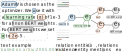
\includegraphics[width=\linewidth]{figures/ref_params/schema_visual_v3}
  \caption[Illustration of hyperparameter information in a text example alongside the extracted entities and relations]{Illustration of hyperparameter information in a text example alongside the extracted entities and relations. Entity types are {\color{artifactblue}{research artifact}}, {\color{parametergreen}{parameter}}, {\color{valuered}{value}}, and {\color{contextgrey}{context}}. Relations are indicated by arrows.}
  \label{fig:schema-visual}
\end{figure}

% - - - - - Why is structured information about hyperparams important? - - - - -

Models capable of extracting fine-grained information from publications can make scientific knowledge machine-readable at a large scale.
Aggregated, such information can fuel platforms like Papers with Code\refurl{https://paperswithcode.com/}{2024-01-10} and the Open Research Knowledge Graph~\cite{orkg1,orkg2}, and thereby facilitate academic search, recommendation,  and reproducibility.
%Potential for impact is especially large in rapidly progressing areas of research, such as machine learning (ML) and related fields. Platforms aggregating extracted information, like Papers with Code~\cite{paperswithcode} and the Open Research Knowledge Graph~\cite{orkg1,orkg2}, allow researchers to quickly gain insights into state-of-the-art approaches, reproduce others' work, and find papers relevant to their research.
Accordingly, a variety of approaches for information extraction~(IE) from scientific text have been proposed~\cite{luan2018scierc,Jain2020scirex,semeval21_task8,semeval22_task12,Dunn2022}.  % / such as ...

% - - - - - What are key shortcomings of current research? (research gap)

However, to the best of our knowledge, no approaches exist for the extraction of structured information on hyperparameter use from publications.
That is, information on \emph{with which parameters} researchers use methods and data. We refer to this information as ``hyperparameter information'' (see Figure~\ref{fig:schema-visual}).
%That is, information on not just what methods and data researchers use, but specifically \emph{with which parameters} they use them. We refer to this information as ``hyperparameter information'' (see Figure~\ref{fig:schema-visual}).
Hyperparameter information is important for several reasons. (1)~First, its existence in a paper is an indicator for reproducibility~\cite{Radd2019} and, when extracted automatically, can improve automated reproduction of results~\cite{sethi2018}. (2)~Second, in aggregate it can inform on both conventions in a field as well as trends over time. (3)~Lastly, it enables more fine-grained paper representations benefiting downstream applications based on document similarity, such as recommendation and search. %
Hyperparameter information is challenging to extract, because (1) it is usually reported in a dense format, (2) often includes special notation, and (3) operates on domain specific text (e.g. ``For Adam we set $\alpha$ and $\beta$ to 1e-3 and 0.9 respectively.'').
%Hyperparameter information is challenging to extract due to the types of entities involved. Research artifacts (e.g. ML models) are domain specific and often referred to by acronym only. Parameters may be referred to by symbol or written out (e.g. ``$\alpha$'' or ``learning rate''), and the symbol renditions are prone to being homographs (e.g. ``k'' in k-means and k-nearest neighbors). Lastly, values can be denoted in several forms such as plain text, e notation, and \LaTeX{} (e.g. ``0.01'', ``1e-2'', and ``\verb|1^{-2}|'').

% further shortcomings (of related work doing IE (albeit not for hyperparameters) from scientific text (which is specific b/c of dense and complex information):
% - only abstracts are considered, not full-text
% - (specific to LLMs:) only models accessible solely via API (usually GPT-3/3.5) are considered

% - - - - - How is this research gap closed? (conceptional) - - - - -

To address the lack of approaches for extracting this type of information, we define the task of ``hyperparameter information extraction'' (HyperPIE) and develop several approaches to it. Specifically, we formalize HyperPIE as an entity recognition (ER) and relation extraction (RE) task. We create a labeled data set spanning a variety of computer science disciplines from machine learning (ML) and related areas. The data set is created by manual annotation of paper full-texts, which is accelerated by a pre-annotation mechanism based on an external knowledge base. Using our data set, we train and evaluate both BERT-based~\cite{devlin2019} fine-tuned models as well as large language models (LLMs).
For the former, we develop a dedicated relation extraction model that achieves an improvement of 29\% $\text{F}_1$ compared to a state-of-the-art baseline.
%For LLMs, we propose to prompt models to output structured data in YAML format rather than JSON, with which we achieve an average improvement of 5.5\% $\text{F}_1$ in entity recognition.
For LLMs, we develop an approach leveraging YAML output for structured data extraction, which achieves a consistent improvement in entity recognition across all tested models, averaging at 5.5\% $\text{F}_1$.
Using our best performing model, we extract hyperparameter information from 
15,000 unannotated papers, and analyze patterns across ML disciplines of how authors report hyperparameters.
%unannotated papers and find that it correlates with external reproducibility indicators, measured through interaction on GitHub with the papers' shared code.
All our data and source code is made publicly available.\refurl{https://github.com/IllDepence/hyperpie}{2024-01-10}
%
% - - - - - List of contributions, shared data, etc. (name numbers, facts, links to data, etc.) - - - - -
%
In summary, we make the following contributions.

\begin{enumerate}
    \item We formalize a novel and relevant IE task (HyperPIE).
    \item We create a high-quality, manually labeled data set from paper full-texts, enabling the development and study of approaches to the task.
    \item We develop two lines of approaches to HyperPIE and achieve performance improvements in both of them over solutions based on existing work.
    \item We demonstrate the utility of our approaches by application on large-scale, unannotated data, and analyze the extracted hyperparameter information.
%    \item To test the soundness of our model's predictions outside of the new evaluation data set, we investigate and affirm correlation with external reproducibility indicators.
\end{enumerate}

In the remainder of this chapter we first discuss related work in Section~\ref{sec:refwork}. We then define the HyperPIE task and describe our data set construction in Section~\ref{sec:hyperpie}. This is followed by the description of our BERT- and LLM-based methods in Section~\ref{sec:methods}. In Section~\ref{sec:experiments} we describe our experiments and results. We conclude with a discussion %of results
and overall summary in Sections~\ref{sec:discussion} and \ref{sec:hyper-conclusion}, followed by an overarching result assessment in Section~\ref{sec:hypepie-assessment}.


\section{Related Work}\label{sec:refwork}

%there are several works that address the extraction of other entity types from academic publications' text. Specifically, previous work seems to focus on the biomedical domain as well as material science~\cite{Choudhary2022,Wornow2023}. In the area of machine learning related literature, there notably are SciERC/SciIE~\cite{luan2018scierc} and SciREX~\cite{Jain2020scirex}, tackling the extraction of ML related enties (datasets, metrics, tasks, methods, etc.), from paper abstracts and full-texts respectively. With the recent advances in large language models (LLMs), there also has been a surge in been efforts to utilize LLMs for IE from scientific text.

% We are not aware of previous research on IE of hyperparameter information. We therefore describe existing work that is concerned with IE of structurally similar information and/or IE approaches in similar application domains.% The related work is grouped into (1) approaches utilizing fine-tuned ML models, and (2) approaches using LLMs.

% general areas of apparent focus on IE from scientific text
% computational linguistics~\cite{semeval18_task7}
% mathematics~\cite{Meadows2022}
% biomedical domain~\cite{Choudhary2022}
% material science~\cite{Wornow2023}

\subsection{Fine-Tuned Models}

% mby short intro paragraph regarding domain specificity

Named entity recognition (NER) and RE from publications in ML and related fields have been tackled by SciERC~\cite{luan2018scierc} and subsequently SciREX~\cite{Jain2020scirex}. The entity types considered are methods, tasks, data sets, and evaluation metrics. Proposed methods for the task utilize BiLSTMs, BERT and SciBERT~\cite{Beltagy2019}. With both approaches, there is a partial overlap in entity types to our task, as we also extract methods and data sets. The key difference arises though the parameter and value entities we cover, which are a challenge in part due to their varied forms of notation (e.g. $\alpha$\,/\,alpha, or $0.001$\,/\,$1\times 10^{-3}$ / 1e-3).

IE models aiming to relate natural language to numerical values and mathematical symbols have been introduced at SemEval 2021 Task 8~\cite{semeval21_task8} and SemEval 2022 Task 12~\cite{semeval22_task12} respectively. Most of the proposed models base their processing of natural language on BERT or SciBERT. To handle numbers and symbols rendered in \LaTeX{}, as well as to accomplish RE between entity types with highly regular writing conventions (e.g. numbers and units such as ``5 ms''), rule-based approaches or dedicated smaller neural networks are commonly used.

Similarly, we find a level of regularity in how authors report parameters and values, and make use of that in our approach accordingly. In line with related work using fine-tuned models, we also use BERT and SciBERT for contextualized token embeddings.

\subsection{LLMs}

With the recent advances in LLMs, there has been a surge in efforts to utilize them for IE from scientific text. Nevertheless, their performance is not on par with dedicated models for NER and RE yet~\cite{Yang2023}.

An important concept for IE with LLMs is introduced by Agrawal et al.~\cite{Agrawal2022}: a ``resolver'' is a function that maps the potentially ambiguous output of an LLM to a defined, task specific output space. In their work, the authors extract singular values and lists from clinical notes using GPT-3. They use a variety of resolvers that perform steps like tokenization, removal of specific symbols or words, and pattern matching using regular expressions.
% - custom output format: list of ``-"medication name"'' lines
% - formalize concept of a ``resolver'', that maps from LLM output to task specific output space

Work with similar output data complexity (values and lists) has also been done in the area of material science. Xie et al.~\cite{Xie2023} use GPT-3.5 to extract information on solar cells from paper full-text.
% For a list of properties to be extracted, they prompt the model to output ``property: value'' lines. The authors note that deviations from the pre-defined format (e.g. the name of a property being slightly changed by the LLM) lead to problems in parsing the LLM output.
% - custom output format: multiple ``schema name: answer'' lines
Similarly, Polak et al.~\cite{Polak2023} use ChatGPT %(also eval GPT-3.5 but performs worse)
to extract material, value, and unit information from sentences of material science papers. They define a conversational progression, in which they prompt the model generate tables, which are processed using simple string parsing rules.
%to extract material, value, and unit information from sentences of material science papers. They define a conversational progression for their IE procedure, in which they prompt the model generate a table and ask confirming follow-up questions on each extracted value. Parsing of the LLM generated table is done using simple string parsing rules.
% - extract Material, Value, Unit
% - use models:
%   - text-davinci-002-render-paid  (ChatGPT)
%   - gpt-3.5-turbo-0301  (ChatGPT)
%   - text-davinci-003  (GPT-3.5)
% - extract data on sentence level
% - perform conversation w/ model

An approach for IE of more complex information is proposed by Dunn et al.~\cite{Dunn2022}. They use GPT-3.5 to extract material information from materials chemistry papers. Given the hierarchical nature of the information to be extracted, the authors find simple output formats insufficient. To overcome this, they prompt the model to output the data in JSON format.\refurl{https://www.json.org/}{2024-01-10}

Given hyperparameter information also is hierarchical (see Figure~\ref{fig:schema-visual}), we adopt prompting LLMs to output data in a text based data serialization format. Different from the related work introduced above, we do not limit our experiments to API access based closed source LLMs, but also evaluate various open LLMs, because we recognize the importance of contributing efforts to the advancement of the more transparent, accountable, and reproducibility friendly side of this new and rapidly evolving area of research~\cite{Liesenfeld2023}.\\
\\
% hyperparam IE from structured sources
% - Baudart2020 - hyperparameter extraction form documentation
%   - Mining Python docstrings to extract hyperparameter schemas including constraints
%   - relies on regularity of docstrings
%   - relies on existence of methods __init__, fit, and predict/transform
%   - use two hand-crafted CNL grammars
% - RakAmnouykit2021 - hyperparameter constraint extraction from code
%   - argue that above (using docstrings) is too vague
%   - focus on Python and sklearn
%   - use static analysis
Besides IE from scientific publications, there have been efforts to extract hyperparameter schemata and constraints from Python docstrings~\cite{Baudart2020} using CNL grammars~\cite{Kuhn2014}, and from Python code~\cite{RakAmnouykit2021} using static analysis. Compared to our task setting, these rely on a known context (e.g. a \texttt{fit} method) and operate on constrained input (generated docstrings and source code instead).

\section{Hyperparameter Information Extraction}\label{sec:hyperpie}

% In this section we define the task of hyperparameter information extraction and describe our data set creation process.

\subsection{Task Definition}

% To illustrate, in the sentence ``During fine-tuning, we use the Adam optimizer with a learning rate of $\alpha = 10^{-4}.$'' (based on text in \cite{Chen2019}) ``Adam optimizer'' is a research artifact,  ``learning rate''/``$\alpha$'' its parameter, ``$10^{-4}$'' the value of the parameter, and ``During fine-tuning'' the context in which the value applies.
%parameter\,$\xrightarrow[]{\text{\tiny used for}}$\,research artifact, value\,$\xrightarrow[]{\text{\tiny used for}}$\,parameter, and context\,$\xrightarrow[]{\text{\tiny used for}}$\,value.

We define HyperPIE as an ER+RE task with four entity classes ``research artifact'', ``parameter'', ``value'', and ``context'', and a single relation type. Briefly illustrated by a minimal example, in the sentence \textit{``During fine-tuning, we use the Adam optimizer with $\mathit{\alpha=10^{-4}}$.''}, the research artifact \textit{Adam} has the parameter $\mathit{\alpha}$ which is set to the value $\mathit{10^{-4}}$ in the context \textit{During fine-tuning}.

The entity classes are characterized as follows. A ``research artifact'', within the scope of our task, is an entity used for a specific purpose with a set of variable aspects that can be chosen by the user. These include methods, models, and data sets.\footnote{Broader definitions in other contexts also include software in general, empirical laws, and ideas~\cite{Lin2022}. For our purposes, however, above specific definition is more useful.} A ``parameter'' is a variable aspect of an artifact. This includes model parameters, but also, for example, the size of a sub-sample of a data set. A ``value'' expresses a numerical quantity and in our task is treated like an entity rather than a literal. Lastly, a ``context'' can be attached to a value if the value is only valid in that specific context. The single relation type relates entities as follows: parameter\,$\rightarrow$\,research artifact, value\,$\rightarrow$\,parameter, and context\,$\rightarrow$\,value.
Co-reference relations %in our scheme
implicitly exist between the mentions of a common entity (e.g. ``AdamW'' and ``it'' in Figure~\ref{fig:schema-visual}). That is, if an entity has multiple mentions within the text, they are considered co-references to each other.

% could mby make an argument for the importance of including context based on ~\cite{Jiang2019}

%\footnote{We note that concrete instantiations of an artifact are treated as metonymic references to the abstract concept itself. For example, in ``X et al. propose the Long short-term memory. We train an LSTM on Y. We evaluate our model on Z.'', ``Long short-term memory'', ``LSTM'' and ``our model'' are all treated as co-references.}

% Since scientific ideas build upon each other, artifacts can include other artifacts, such as transformer models utilizing attention, and attention in turn utilizing softmax.

% general discussion of challenges in finding balance between applicability and expressiveness

% NOTES:
% refer to concept of "salient entities" (SciREX paper) -> those that are "taking part in the article evaluation" / "needed to describe the article's results"

% Part-of (beta1$\rightarrow$ADAM$\rightarrow$LSTM) out of scope b/c models already exist (SciERC, etc. $\rightarrow$ apply both models, have full info)


The scope of the IE task comprises the extraction of entities, their relations, and the identification of all their mentions in the text (and thereby implicitly co-references). %The task does not involve mention/use classification or saliency classification. 
Furthermore, we specifically consider IE from text, and not from tables, graphs, or source code.\footnote{We leave investigating multi-modal IE pipelines (text/code/graphs) for future work.}

\subsection{Data Set Construction}\label{sec:data-set-contruction}

% data selection: chose from various ``ML fields'' such as cs.CL, cs.LG, cs.CV. cs.DL to ensure capturing a wide variety of common artifacts as well as discipline specific writing conventions

% To ensure X, Y, and Z (value of initial investigation is that design of the data scheme is ``compatible'' with real world data) (also convey that domain expertise and related work were a basis, but initial investigation is a plus on top of that)

% Our initial annotation scheme and guidelines are informed by related work~\cite{Jain2020scirex,luan2018scierc}.

% \begin{itemize}
%     \item we follow the ACL RD-TEC 2.6 guidelines~\cite{Qasemizadeh2016} for term boundaries
%     \item greedy annotation, maximal length annotation principle 
%     \item no determiners
%     \item no pronouns (``our model'' $\rightarrow$ ``model'')
% \end{itemize}

Because HyperPIE is a novel task, we cannot rely on existing data sets for training and evaluating our approaches. We therefore create a new data set by manually annotating papers. As our data source we chose unarXive~\cite{Saier2023unarXive}, because it includes paper full-texts and, most importantly, retains mathematical notation as \LaTeX{}. This is crucial because parsing such notation from PDFs is prone to noise, which would be problematic for our parameter and value entities.  % reference would be nice here (Bast2017 focus is on text only)

% cs.LG, cs.CL, cs.CV, cs.DL = 143,203 papers (number from get_plaintext_paras.py)
To ensure we cover a wide variety of artifacts and discipline specific writing conventions, we use papers from multiple ML related fields. Specifically, these are Machine Learning (ML), Computation and Language (CL), Computer Vision (CV), and Digital Libraries (DL), which make up 143,203 papers in unarXive.\footnote{The respective arXiv categories are cs.LG, cs.CL, cs.AI, and cs.DL. See \refurlinline{https://arxiv.org/category_taxonomy}{2024-01-10} for a more detailed description.}

We base our annotation guidelines on the widely used ACL RD-TEC guideline\refurl{https://web.archive.org/web/20220120204209/http://pars.ie/publications/papers/pre-prints/acl-rd-tec-guidelines-ver2.pdf}{2024-01-10}~\cite{Qasemizadeh2016}. To make sure our resulting annotations are able to properly capture how authors report hyperparameters in text, we perform two annotation rounds: (1) an initial exploratory round, the results of which are used to refine the annotation guidelines and inform later model development, and (2) the main annotation round, the results of which constitute our data set used for model training and evaluation. In the following, both steps are described in more detail.

\subsubsection{Initial Annotation Round}\label{sec:exploreannot}

% data selection: heuristic pre-filtering for hyperparam descriptions (details in appendix)
% heuristics
% - has_math (=LaTeX)
% - has_display_math (used as negative filter)
% - has_num
% - has_indicator_phraes
%     re.search(r'we(\s+have)? (use|chos|set)', s, flags=re.I) or \
%           'set to' in s or \
%           'set the' in s or \
%           ('set' in s and 'parameter' in s) or \
%           ('use' in s and 'parameter' in s) or \
%           ('set' in s and 'factor' in s) or \
%           ('use' in s and 'factor' in s) or \
%           ('use' in s and 'setting' in s) or \
%           ('set' in s and 'value' in s) or \
%           ('use' in s and 'value' in s) or \
%           (quick_math and '=' in s):
% if has_math and \
%         has_num and \
%         has_indicator_phraes and \
%         not has_display_math:
% not used:
% - has_var_assignment (len(plain_math) < 15 and '=' in f_dict['latex'])
% - quick_math (len(plain_math) < 7)

We heuristically pre-filter our ML paper corpus for sections reporting on hyperparameters.\footnote{We filter based on key phrases (``use'', ``set'', etc.), numbers, and \LaTeX{} math content.} Annotators then inspect these sections, select a continuous segment of text that contain hyperparameter information, and make their annotations. This task is performed independently by two annotators and results in a total of 151 text segments (131 unique, $2\times10$ annotated by both). The annotated text segments contain 1,345 entities and 1,110 relations.

\begin{figure}
    \centering
    \subfloat[text segments\label{fig:text-seg-size}]{%
        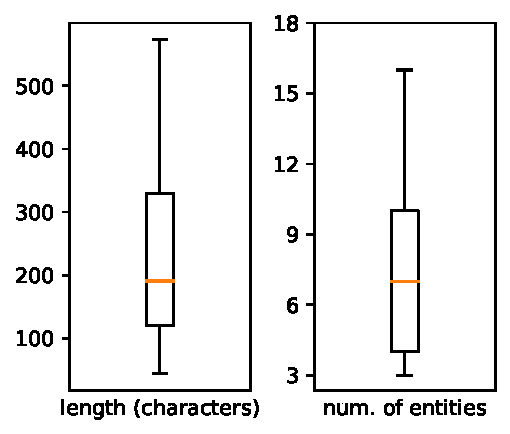
\includegraphics[width=.35\linewidth]{figures/ref_params/text_span_size_stats}
    }
    \subfloat[relation distances (\#chars)\label{fig:rel-dists}]{%
        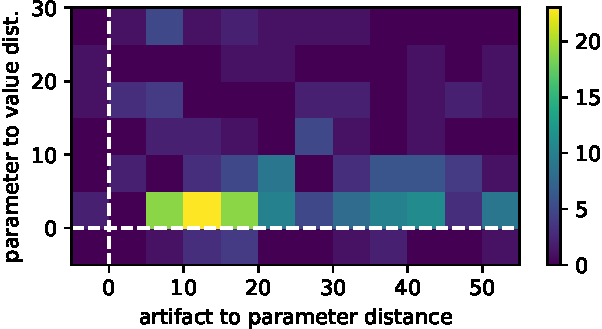
\includegraphics[width=.53\linewidth]{figures/ref_params/stats_artifact_param_value_distance-crop}
    }
    \caption{Observations of initial annotation round}
    \label{fig:init-annot}
\end{figure}

% basic stats on character lenghts of continuous text segments

% count     151.000000
% mean      269.834437
% std       233.249350
% min        44.000000
% 25%       121.000000
% 50%       191.000000
% 75%       330.000000
% max      1262.000000

% basic stats on entity count within a continuous text segment

% count    151.000000
% mean       8.907285
% std        7.693591
% min        3.000000
% 25%        4.000000
% 50%        7.000000
% 75%       10.000000
% max       49.000000

% full unarXive × PwC data paragraph length:
% average 563.5783976547118   (based on 9,566,415 paragraphs)

% param after artifact: 457/587 (78%)
% param before artifact: 130/587 (22%)
% mean: 45.89, std: 130.28
% value after param: 548/587 (93%)
% value before param: 39/587 (7%)
% mean: 15.73, std: 25.98

As shown in Figure~\ref{fig:text-seg-size}, we observe text segments reporting on hyperparameters to generally have a length below 600 characters. %, with a mean of 269.8 (standard deviation 233.2) and median of 191.
We furthermore see that most text segments contain between 3 and 15 entities. % (mean 8.9, median 7).
Lastly, in Figure~\ref{fig:rel-dists}, show distances between artifacts and their parameters, as well as parameters and their values. We see that artifacts usually are mentioned before their parameters (78\%), and parameters before their values (93\%). The reverse cases also exists, but are less common.
Additionally, we can see that values are most commonly reported right after their parameter, while there is a higher variability in distances between parameters and artifacts.
% The mean absolute distance is 51.6.
Based on above observations % on (1) the length of text segments reporting hyperparameter information, and (2) relation distances between the entities concerned,
we determine the unit of annotation for the final round to be one paragraph (on average 563.4 characters long in our corpus), as it is sufficient to capture hyperparameters being reported.
%can safely set the unit of annotation for the final round to be one paragraph.\footnote{The average paragraph length for the whole paper corpus is 563.4 characters.}

The inter annotator agreement (IAA, reported as Cohen's kappa) of the text segments annotated by both annotators is 0.867 for entities and 0.737 for relations\footnote{Measured by the character level entity class and character level relation target span agreement respectively.} (strong to almost perfect agreement) which is compares favorably to SciERC~\cite{luan2018scierc} with an IAA of 0.769 for entities and 0.678 for relations.

% initial investigation stats

% 151 annotated text segments (131 unique), annotated by two annotators
% 1,345 annotated entities
% 1,110 annotated relations
% inter annotator agreement (based on 20 text segments annotated by both annotators)
%   entities
%     Cohen’s kappa based on character level entity class: 0.867
%     exact match of entity spans: 105/133 (0.789)
%   entities + relations
%     Cohen’s kappa based on character level relation target span : 0.737
%     exact match of relations and their exact entity spans: 88/132 (0.667)

\subsubsection{Main Annotation Round}

% to make the annotation process more efficient text is pre-annotated using (1) the annotator's previous artifact and parameter annotations, and (2) simple regex patterns for numeric values (candidates for parameter values).

In our main annotation round we annotate whole papers (paragraph by paragraph) instead of pre-filtered text-segments. This is done to ensure that the final annotation result reflects data as it will be encountered by a model during inference---that is, containing a realistic amount of paragraphs that have no information on hyperparameters, or, for example, only mention research artifacts but no parameters.

Similar to related work~\cite{Jain2020scirex}, we use Papers with Code as an external knowledge base to pre-annotate entity candidates to make the annotation process more efficient. In a similar fashion, we use annotator's previously annotated entity mentions for pre-annotation. Pre-annotated text spans are, as the name suggests, set automatically, but need to be checked by annotators manually.

Through this process we annotate 444 paragraphs, which contain 1,971 entities and 614 relations. The entity class distribution is 1,134 research artifacts, 131 parameters, 662 values, and 44 contexts. The annotation data is provided in a JSON structure as shown in Figure~\ref{fig:schema-visual}, as well as in the W3C Web Annotation Data Model\refurl{https://www.w3.org/TR/annotation-model/}{2024-01-10} to facilitate easy re-use and compatibility with existing systems.

% 444 annotated paragraphs
% 1,971 entities
% 614 relations (212 used for, 402 co-relation (*counted as “to first mention, not n-to-n))



\section{Methods}\label{sec:methods}

We approach hyperparameter information extraction in two ways. First, we build upon established ER+RE methods and develop an approach using a fine-tuned model in a supervised learning setting. Second, given the recent promising advances with LLMs, we develop an approach utilizing LLMs in a zero-shot and few-shot setting.

\subsection{Fine-Tuned Models}

% - - - Fine-tuned - - -
% - use SciERC SOTA PL-Marker: NER good, RE bad
% - based on initial annotation round observation (regularity in rel dist)
%   + entity class combo determinism: implement RE w/ reldist+class focus
%
% note that large variance in cross-eval results is due to varying class imbalance on test set b/c data is split stratified by paper

% Despite the recent success of LLMs in a range of NLP tasks, smaller fined-tuned models still outperform them in the case of NER and RE~\cite{Yang2023}.

We base our fine-tuned model approach on PL-Marker~\cite{Ye2022}, the currently best performing model on SciERC. Specifically, we use the ER component of PL-Marker. Our reason is that (1)~the text our model will be applied on is of the same type as in SciERC (ML publications), and (2)~there is some correspondence between the entities to be identified---namely our entity class ``research artifact'' including methods and datasets, which are both entity classes in SciERC.

For RE we develop an approach that utilizes token embeddings as well as relative entity distance and entity class pairings. This is motivated by the fact that (a) we observed a high level or regularity in the relative distance of research artifact, parameter, and value mentions\footnote{We note that these observations where made during the initial exploratory annotation round (Section~\ref{sec:exploreannot}) and not during annotation of the evaluation data.} (see Figure~\ref{fig:init-annot}), and (b) relations only exist between specific pairs of entity types.

\begin{figure}[bt]
  \centering
  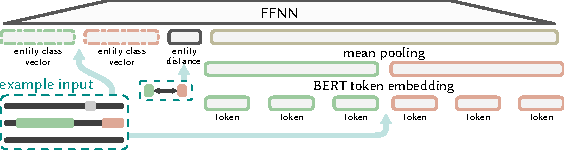
\includegraphics[width=.8\linewidth]{figures/ref_params/ffnn_re_sub_visual_v2}
  \caption{Relation extraction with emphasis on entity candidate pair types and distance.}
  \label{fig:ffnn-re-sub-visual}
\end{figure}

In Figure~\ref{fig:ffnn-re-sub-visual} we show a schematic depiction of our new relation extraction component. Entity candidate pair classes as well as the relative distance between the entities in the text are used as a dedicated model input, BERT token embeddings of the entity mentions are combined using mean pooling. These inputs are fed into a feed-forward neural network FFNN for prediction. Formally, the model performs pairwise binary classification as $\text{FFNN}(E^c_0, E^c_1, E^d, E^T)$, where $E^c_i$ are class vectors, $E^d$ encodes candidate distance, and $E^T$ is the token pair embedding calculated as $E^T=\frac{1}{|T|}\sum^{|T|}_{i=0}\text{BERT}(t_i)$, the mean of the pair's tokens $t_i\in|T|$.

% FFNN implemented with 4 hidden layers, each with ReLU activation and dimensions 300, 100, 25 and 2 respectively

During the development of our model we also experiment with concatenation in favor of mean pooling to preserve information on the order of the entities, but find that mean pooling results in better performance. Furthermore, we investigated the use of SciBERT instead of BERT, but find that regular BERT embeddings give us better results, despite our model handling scientific text.

% Implementation details for both the PL-Marker ER component as well as the RE component can be found in Appendix~\ref{sec:implementation-details}.

\subsection{LLMs}\label{sec:methLLMs}

We develop our LLM approach for a zero-shot and a few-shot setting. This means the models perform the IE task based on either instructions only (zero-shot), or instructions and a small number of examples (few-shot).

% common approaches
% - chaining (identify entities, identify mentions, identify relations) (ex.: Wu2022)
% - seq2seq (mark entities with types/IDs within text)
% - using serialization format as output

% common prompt structures/techniques
% - [task][few shot examples][input] (ex.: Wang2023)
% - chain of though prompting (ex.: Kojima2022)

% ~\cite{Kojima2022} specify format input (e.g. ``The answer (arabic numerals) is''m or ``Among A through E, the answer is'') and also do ``answer cleansing''

% Using LLMs to extract structured data from natural language text, means that at a transition has to be achieved from the ambiguous realm of natural language to precisely defined structures. 

Performing IE using LLMs in zero-shot or few-shot settings requires the desired structure of the output data to be specified within the model input. In simple cases (e.g. numbers or yes/no decisions) this can be achieved by an in-line specification of the format in natural language (e.g. ``The answer (Arabic numerals) is'')~\cite{Kojima2022}. IE from scientific publications, however, often seeks to extract more complex information. To achieve this, the model can be tasked to produce output in a text based data serialization format such as JSON, as done in previous work~\cite{Dunn2022}. Especially for complex structured predictions, few-shot prompting has been shown to further boost in-context learning (ICL) accuracy and consistency at inference time~\cite{Brown2020gpt3}.

Drawing from techniques used in previous work approaching other IE tasks, we investigate several prompting strategies to build our approach.
%
% try
% - few shot
% not feasible b/c context length
% - multi stage prompt
% but leads to worse results (assume b/c context has to be re-established
% each iteration, increasing potential for errors/loss of information)
% - "infilling" type prompt
% but LLM changes text
% - infilling after extraction
% but LLM hallucinates/is inconsistent with entity identifiers (e.g. marks an
% entity "a6" when there is only a1 to a5 in extracted data)
%

\begin{enumerate}
    \item \textit{Multi-stage prompting}~\cite{Polak2023}: first determine the presence of hyperparameters information; if present, extract the list of entities; lastly, determine relations.
    \item \textit{In-text annotation}~\cite{Wang2023}: let the input text be repeated with entity annotations, e.g. repeat ``We use BERT for ...'' as ``We use [a1|BERT] for ...''. %, where ``a'' indicates entity class ``artifact'' and ``1'' is the entity ID.
    \item \textit{Data serialization format}~\cite{Dunn2022}: specify a serialization format in the prompt that is parsed afterwards; then match in-text mentions in the input.
    \item \textit{(3)+(2)}: prompt as in (3); then match in-text mentions using (2).
\end{enumerate}

% We find that for (1) the higher number of steps leads to more points of potential errors being introduced and then propagated, and an overall less robust pipeline. In the case of (2) and (4) we see frequent changes in the reproduced annotated text posing significant challenges in making use of the output. Accordingly, we use prompt type (3) for our approach.
We find (1) to lead to problems with errors propagation along steps. With (2) and (4) we frequently see alterations in the reproduced text. Accordingly, we use prompt type (3) for our approach---specifying a data serialization format in the prompt.
While existing work uses the JSON format for this~\cite{Dunn2022}, we use YAML, as it is less prone to ``delimiter collision'' problems due to its minimal requirements for structural characters.\refurl{https://yaml.org/spec/1.2.2/}{2024-01-10} 
In doing so, we expect to avoid problems with LLM output not being parsable. Our overall LLM approach looks as follows.
%
% Because YAML primarily relies on outline indentation for structure, it is especially resistant to delimiter collision. (https://en.wikipedia.org/wiki/YAML#Indented_delimiting | https://en.wikipedia.org/wiki/Delimiter#Delimiter_collision)
%

\subsubsection{Zero-shot} We build our zero-shot prompts from the following consecutive components: \texttt{[task]\allowbreak[input text]\allowbreak[format]\allowbreak[completion prefix]}.
An example is shown in Appendix~\ref{app:hyperpie-implementation-details}.
In \texttt{[task]} we specify the information to extract, i.e., research artifacts, their parameters, etc. \texttt{[input text]} is the paragraph from which to extract the information. \texttt{[format]} defines the output YAML schema. \texttt{[completion prefix]} is a piece of text that directly precedes the LLM's output, such as \textit{``ASSISTANT:~''}.
%
% Also: in case of maximum output length being reached, “fixing” is trivial by removing last (potentially incomplete line), whereas fixing JSON to make it parsable is more involved (need matching delimiters
%
To generate predictions based on LLM output, we pass it to a standard YAML parser after cleansing (e.g. removing text around the YAML block).
%
% To generate predictions based on the LLM output, we parse the YAML output\footnote{Note that this is not a custom procedure but means simply using the YAML parsing functionality in a programming languages standard library (in our case Python).} after cleansing (e.g. removing unwanted text before or after the YAML block) and transform it into the format used in the evaluation or downstream application.
%
For each used LLM model, we individually perform prompt tuning. Here we determine, for example, if a model gives better results when the \texttt{[completion prefix]} includes the beginning of the serialized output (e.g., ``\texttt{-{}-{}-\allowbreak\textbackslash n\allowbreak text\_\allowbreak contains\_\allowbreak entities:}'') or if this leads to a deterioration in output quality.

\subsubsection{Few-shot} Our few-shot approach makes the following adjustments to the method described above. Prompts additionally include a component \texttt{[examples]}, which are valid input output pairs sampled by their cosine similarity to the input text. Specifically, for an input text from a document X, we sample the five most similar paragraphs from all ground truth documents excluding X. As these examples can be confused with the input text, we re-position the input text to appear \emph{after} the examples. The resulting prompt structure we use for our few-shot approach is as follows: \texttt{[task]\allowbreak[format]\allowbreak[examples]\allowbreak[input text]\allowbreak[completion prefix]}.
An example is shown in Appendix~\ref{app:hyperpie-implementation-details}.

LLMs reaching a sufficient context size for a few-shot approach to our task are a recent development. We can therefore additionally make use of other recently added capabilities. Specifically, we make use of generation constrains via a gBNF grammar\refurl{https://github.com/ggerganov/llama.cpp/pull/1773}{2024-01-10} to enforce LLM output according to our data scheme, allowing us to mitigate parsing errors.

\section{Experiments}\label{sec:experiments}

We evaluate the fine-tuned models and LLM approach against baselines from existing work. Both evaluations are performed on our data set described in Section~\ref{sec:data-set-contruction}. Metrics used to measure prediction performance are precision, recall and $\text{F}_1$ score, abbreviated as P, R and $\text{F}_1$ respectively.

\subsection{Fine-Tuned Models}

% (side note: in PL-Marker data conversion, 93% of annotation boundaries
%  exactly match a token boundary — therefore comparison is more realistic
%  between LLM zero shot *exact match* and PL-Marker results)
% Annotation boundary exactly matches token boundary: 3,786 (0.93)
% Annotation boundary lies within token boundary: 266 (0.07)

We use PL-Marker, the currently best performing model on SciERC, as our baseline.
% As both PL-Marker and our model work on the level of tokens, whereas the evaluation data has annotations with character level granularity, we first convert the data to a tokenized format. 93\% of the annotation boundaries exactly match token boundaries.
% (possible example for difference: token “5-fold” w/ only “5” annotated as value)
Models are trained and evaluated using 5-fold cross validation (3 folds training, 1 dev, 1 test).
%
% We also experiment with splitting the data into folds obtained by sampling whole papers (i.e., the complete set of paragraphs of each paper) rather than individual paragraphs. We do this to ensure a realistic evaluation setting and prevent, for example, directly subsequent paragraphs of a paper being split up into training and testing data. This has the side effect that class distributions across the 10 evaluation runs vary considerably---in other words, some folds contain considerably fewer entities and/or relations to extract than others. As a consequence, model performance varies between splits, leading to high standard deviations in the evaluation metrics.
%
We train the ER component of PL-Marker as done in~\cite{Ye2022}, using \textit{scibert-scivocab-uncased} as the encoder, Adam as the optimizer, a learning rate of 2e-5, and 50 training epochs. Regarding the two RE components we compare, the PL-Marker RE component is trained using \textit{bert-base-uncased}, Adam, a learning rate of 2e-5, and 10 training epochs. Our own RE component also uses \textit{bert-base-uncased}, Adam as the optimizer, and is trained with a learning rate of 1e-3 for 90 epochs.\footnote{The two RE models we compare require different learning rates and number of training epochs, because their architecture varies significantly.}
The models are trained and evaluated on a server with a single GeForce~RTX~3090 (24\,GB).\footnote{More extensive implementation details can be found in Appendix~\ref{app:hyperpie-implementation-details}.}

% run_acener.py
% learning_rate 2e-5
% num_train_epochs 50
% per_gpu_train_batch_size 8
% per_gpu_eval_batch_size 16
% gradient_accumulation_steps 1
% max_seq_length 512
% max_pair_length 256
% max_mention_ori_length 8
% run_acener.py:    optimizer = AdamW(optimizer_grouped_parameters, lr=args.learning_rate, eps=args.adam_epsilon)

% run_re.py
% learning_rate 2e-5
% num_train_epochs 10
% per_gpu_train_batch_size 8
% per_gpu_eval_batch_size 16
% gradient_accumulation_steps 1
% max_seq_length 256
% max_pair_length 16
% run_ner.py:    parser.add_argument("--adam_epsilon", default=1e-8, type=float,

% solver='adam',
% learning_rate_init=0.001,
% max_iter=10000,  (For stochastic solvers (‘sgd’, ‘adam’), note that this determines the number of epochs)
% trained until 10 consecutive epochs loss does not improve by at least 1e-4

\subsubsection{Results}

% % PL
% % NER precision: 81.5 ± 2.9
% % NER recall: 76.8 ± 2.2
% % NER f1: 79.0 ± 1.6
% % RE precision: 33.5 ± 19.3
% % RE recall: 5.9 ± 3.7
% % RE f1: 9.9 ± 6.0

% % FFNN
% % RE precision: 30.7 ± 11.1
% % RE recall: 65.0 ± 32.4
% % RE f1: 38.8 ± 11.3

\begin{figure}[tb]
  \centering
  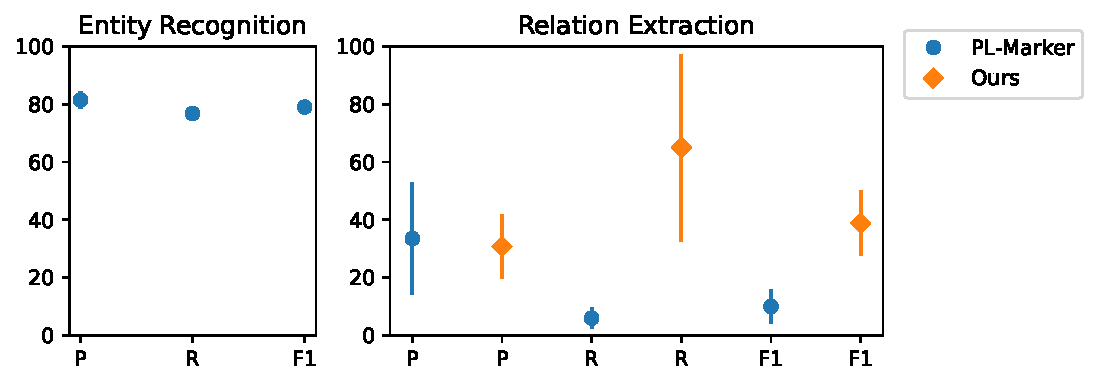
\includegraphics[width=.8\linewidth]{figures/ref_params/fine_tuned_eval}
  \caption{Fine-tuned model evaluation (5-fold cross validation).}
  \label{fig:finetunedeval}
\end{figure}

In Figure~\ref{fig:finetunedeval} we show the results of PL-Marker ER (used for both models) as well as the PL-Marker RE component and our RE model. For ER we evaluate exact matches (no partial token overlap). In the case of RE, each entity pair is predicted as having a relation or not---as there is just one relation type.

Mean ER performance is 81.5, 76.8, and 79.0 (P, R, $\text{F}_1$). For RE, the precision of PL-Marker and our model are similar at 33.5 and 30.7 respectively, but our model performs more consistent. PL-Marker only achieves a very low recall of 5.9, whereas our model, while showing large variability, achieves a mean of 65.0. The resulting $\text{F}_1$ scores are 9.9 for PL-Marker and 38.8 for our model.

%We take this indication that overall the ER part of hyperparameter IE is comparatively difficult as more general IE from computer science publications. % TODO: discuss class differences if space allows (see figure below)

% \begin{figure}[tb]
%   \centering
%   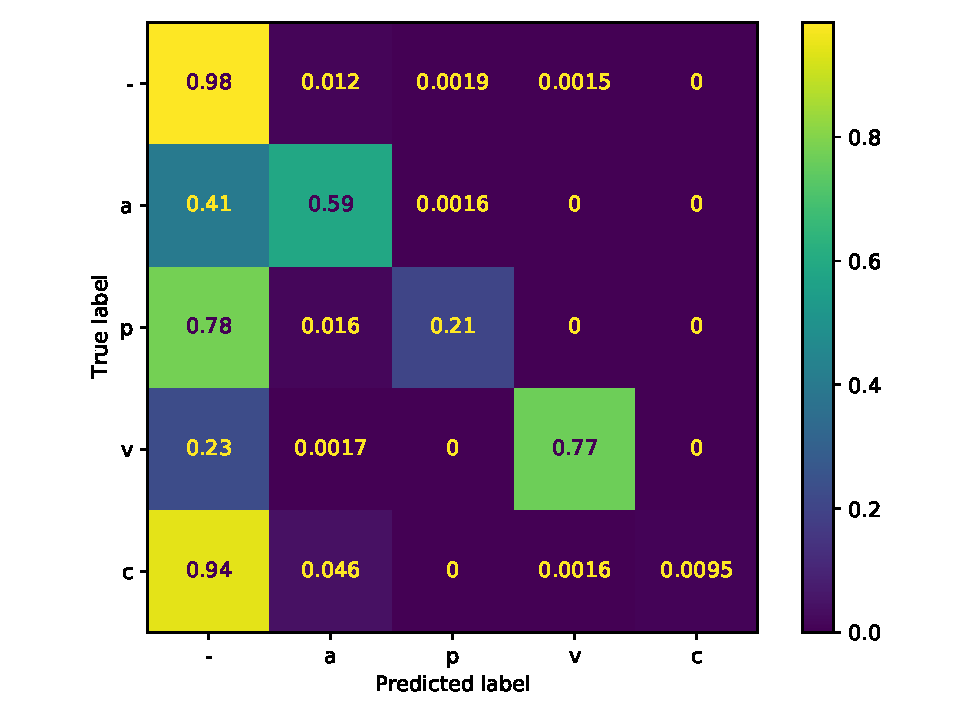
\includegraphics[width=\linewidth]{figures/ref_params/ner_confusion_matrix}
%   \caption{ER confusion matrix for PL-Marker evaluation}
%   \label{fig:plmrk-confusion}
% \end{figure}

% NER confusion matrix in Figure~\ref{fig:plmrk-confusion}.

% \subsubsection{Error Analysis}

% Analysing the ER predictions in our evaluation, we find that the worst performing entity class is ``context'' with 94\% false negatives. Given context boundaries can be fuzzy and our evaluation is for exact matches, partial match or manual evaluation could be an alternative. 

\subsubsection{Analysis}

% ER F1s per class (token level):
% (labels = none, artifact, parameter, value, context)
% $\text{F}_1$ scores to be 98.5\%, 77.8\%, 47.9\%, 84.4\%, 0\%

% ### with everything
% RE precision: 30.7 ± 11.1
% RE recall: 65.0 ± 32.4
% RE f1: 38.8 ± 11.3

% ### no bert embeddings (adjusted network size** ((300, 100, 25, 2) -> (25, 5, 2)))
% RE precision: 15.5 ± 22.6
% RE recall: 8.8 ± 12.2
% RE f1: 11.1 ± 15.7

% ### no relative distance
% RE precision: 26.5 ± 8.2
% RE recall: 65.0 ± 28.5
% RE f1: 35.5 ± 9.7

% ### no token class embeddings (adjust bert embedding weight to 0.5)
% RE precision: 16.6 ± 16.1
% RE recall: 29.8 ± 33.0
% RE f1: 19.6 ± 18.0
\begin{table}
  \centering
  \caption[Ablation study results]{Ablation study results (model inputs are: T = BERT token embeddings, C = entity class embeddings, D = entity distance)}
  \label{tab:finetunedablation}
  \begin{tabular}{lccc}
    \hline
    Model inputs used & P [\%] & R [\%] & $\text{F}_1$\,[\%] \\
    \hline
    \textvisiblespace CD & 15.5 & 8.8 & 11.1 \\
    T\textvisiblespace D & 16.6 & 29.8 & 19.6 \\
    TC\textvisiblespace & 26.5 & 65.0 & 35.5 \\
    TCD & \textbf{30.7} & \textbf{65.0} & \textbf{38.8} \\
    \hline
  \end{tabular}
\end{table}

Token level ER performance across entity classes (none, artifact, parameter, value, context) is at 98.5\%, 77.8\%, 47.9\%, 84.4\%, 0\% $\text{F}_1$. That is, the model does not predict contexts and struggles with parameters, but artifacts and values are predicted reliably. For our RE model, we observe that value-parameter relations are more reliably predicted than parameter-artifact relations.

\begin{figure}
  \centering
  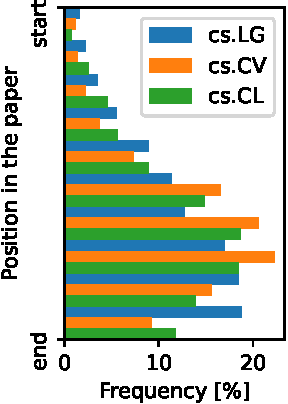
\includegraphics[width=0.3\linewidth]{figures/ref_params/hyperparam_pos-crop}
  \caption{Frequency of hyperparameter mention positions in papers.}
  \label{fig:hyperparam_info_pos}
\end{figure}

% cs.LG: 0.35890524569769855
% cs.CV: 0.41702606412900806
% cs.CL: 0.36408882082695254
% cs.DL: 0.06666666666666667

To assess the impact of the different components in our RE model, we perform an ablation study with the same 5-fold cross-validation setup as above. In Table~\ref{tab:finetunedablation}, showing its results, we can see that removing the BERT token embeddings (T) results in the largest performance loss, followed by entity class embeddings (C) and entity distance (D). Removing any of the inputs results in worse predictions.

Finally, we apply our full model to a random sample of 15,000 papers. Analyzing the results, we find hyperparameters (artifact, parameter, value triples) are reported in 36\% of ML papers, 42\% of CV papers, 36\% of CL papers, and 7\% of DL papers. In Figure~\ref{fig:hyperparam_info_pos} we further look at the distribution of the information across the length of papers (excluding DL as not being representative). We can see a clear tendency towards the latter half of papers.

% \subsubsection{Application}

% We train a final ER+RE model on all annotated data and use it to extract hyperparameter information from a random sample of 15,000 papers. To test the soundness of the extracted information, we test its predictive strength for the re-use of code shared with each paper. Our method assumes that re-use of code is an indicator for reproducibility. For hyperparameter reporting, this has been shown in previous work~\cite{Radd2019}.

% We operationalize the two measures as follows. $r_\text{hype} =$ amount of hyperparameter information, measured as the number of extracted value-parameter, parameter-artifact, and value-parameter-artifact relation ``chains''. $r_\text{code} =$ code re-use, measured as the number of GitHub forks and closed issues, normalized by the number of stars. Normalization is done to control for the influence of author and affiliation renownedness.

% Measuing the correlation between $r_\text{hype}$ and $r_\text{code}$, we find the Pearson correlation coefficient to be 0.x (p=0.00y), a (weak/moderate/strong) positive correlation that is statistically relevant. We interpret our finding as an indicator that the hyperparameter information extracted by our model is sound, but note that additional testing is necessary to draw more definitive conclusions.

\subsection{LLMs}

\begin{table}[tb]
\centering
  \caption[LLM selection]{LLM selection (size in number of parameters).}
  \label{tab:llmselection}
  \begin{tabular}{llc}
    \hline
    Model & Variant & Size \\
    \hline
    WizardLM~\cite{xu2023wizardlm2023}
    & \texttt{WizardLM-13B-V1.1} & 13\,B \\
    Vicuna${}_{4k}$~\cite{vicuna2023}
    & \texttt{vicuna-13b-v1.3} & 13\,B \\
    Vicuna${}_{16k}$~\cite{vicuna2023}
    & \texttt{vicuna-13b-v1.5-16k} & 13\,B \\
    Falcon~\cite{falcon40b-huggingface}
    & \texttt{falcon-40b-instruct} & 40\,B \\
    GALACTICA~\cite{GALACTICA2022}
    & \texttt{galactica-120b} & 120\,B \\
    GPT-3.5~\cite{Brown2020gpt3}
    & \texttt{text-davinci-003} & 175\,B \\
    \hline
    \end{tabular}
\end{table}

For our LLM experiments we chose a variety of models, with sizes ranging from 13\,B to 175\,B parameters, as shown in Table~\ref{tab:llmselection}.
% We specifically evaluate not only proprietary models restricted to API access, but also a open LLMs.
We chose WizardLM~\cite{xu2023wizardlm2023} as it is meant to handle complex instructions, 
Vicuna~\cite{vicuna2023} due to its performance relative to its size, 
Falcon~\cite{falcon40b-huggingface} because of its alleged performance, 
and GALACTICA~\cite{GALACTICA2022} because it was trained on scientific text.
Vicuna${}_{16k}$ is a model extended using Position Interpolation~\cite{chen2023} based on Rotary Positional Embeddings~\cite{su2021}, which makes it the only model in our experiments with a sufficient context size for a few-shot evaluation.

The models are run as follows. GPT-3.5 is accessed through its official API.
% The total usage cost for all testing, prompt tuning, and the full evaluation runs sums up to 60\,USD.
All open models are run on a high performance compute cluster.
% using the API layer Basaran.\footnote{See \url{https://github.com/hyperonym/basaran/}.}
Vicuna${}_{4k}$ and WizardLM are run on nodes with $4\times$NVIDIA Tesla V100 (32\,GB).
GALACTICA, Falcon, and Vicuna${}_{16k}$ are run on nodes with $4\times$NVIDIA A100 (80\,GB).\footnote{More extensive implementation details can be found in Appendix~\ref{app:hyperpie-implementation-details}.}

As a baseline, we use a JSON variant for each model, where the \texttt{[format]} and \texttt{[examples]} compontents of prompts use JSON, and compare it to the respective YAML version. All models are used with greedy decoding (temperature = 0) for the sake of reproducibility.

% Accordingly, only one completion is created per prompt. We evaluate the models on three levels. (1) Parsing success and format adherence, meaning if the produced JSON/YAML was parsable and according to the specified format, (2) hallucinations and scope adherence, where we measure hallucinated and out of scope entities, and (3) prediction performance in terms of precision, recall, and $\text{F}_1$ score.

% TODO: consider explicitly mentioning that b/c the data set is new, there’s no

\subsubsection{Results}

% === Falcon_json ===
% - exact -
% entity_recognition_classification [%]: P: 37.1 R: 5.9 F1: 10.2
% relation_extraction [%]: P: 0.0 R: 0.0 F1: 0.0

% - partial_overlap -
% entity_recognition_classification [%]: P: 48.0 R: 7.7 F1: 13.3
% relation_extraction [%]: P: 0.0 R: 0.0 F1: 0.0

% === Falcon ===
% - exact -
% entity_recognition_classification [%]: P: 32.7 R: 14.2 F1: 19.8
% relation_extraction [%]: P: 0.0 R: 0.0 F1: 0.0

% - partial_overlap -
% entity_recognition_classification [%]: P: 40.6 R: 17.3 F1: 24.2
% relation_extraction [%]: P: 0.0 R: 0.0 F1: 0.0

% === GALACTICA_json ===
% - exact -
% entity_recognition_classification [%]: P: 25.9 R: 15.7 F1: 19.5
% relation_extraction [%]: P: 0.1 R: 2.3 F1: 0.3

% - partial_overlap -
% entity_recognition_classification [%]: P: 34.1 R: 18.4 F1: 23.9
% relation_extraction [%]: P: 0.2 R: 3.1 F1: 0.4

% === GALACTICA ===
% - exact -
% entity_recognition_classification [%]: P: 23.1 R: 19.5 F1: 21.1
% relation_extraction [%]: P: 0.0 R: 0.8 F1: 0.1

% - partial_overlap -
% entity_recognition_classification [%]: P: 31.7 R: 24.6 F1: 27.7
% relation_extraction [%]: P: 0.1 R: 1.5 F1: 0.1

% === WizardLM_json ===
% - exact -
% entity_recognition_classification [%]: P: 6.9 R: 11.3 F1: 8.6
% relation_extraction [%]: P: 0.1 R: 0.8 F1: 0.1

% - partial_overlap -
% entity_recognition_classification [%]: P: 8.6 R: 13.3 F1: 10.4
% relation_extraction [%]: P: 0.1 R: 1.5 F1: 0.2

% === WizardLM ===
% - exact -
% entity_recognition_classification [%]: P: 9.7 R: 35.6 F1: 15.3
% relation_extraction [%]: P: 0.1 R: 1.5 F1: 0.1

% - partial_overlap -
% entity_recognition_classification [%]: P: 12.6 R: 44.4 F1: 19.7
% relation_extraction [%]: P: 0.2 R: 6.1 F1: 0.4

% === Vicuna_json ===
% - exact -
% entity_recognition_classification [%]: P: 15.1 R: 9.3 F1: 11.5
% relation_extraction [%]: P: 0.7 R: 3.8 F1: 1.2

% - partial_overlap -
% entity_recognition_classification [%]: P: 18.5 R: 11.2 F1: 13.9
% relation_extraction [%]: P: 0.8 R: 4.6 F1: 1.4

% === Vicuna ===
% - exact -
% entity_recognition_classification [%]: P: 17.3 R: 31.5 F1: 22.3
% relation_extraction [%]: P: 0.1 R: 0.8 F1: 0.1

% - partial_overlap -
% entity_recognition_classification [%]: P: 20.7 R: 37.0 F1: 26.5
% relation_extraction [%]: P: 0.1 R: 0.8 F1: 0.1

% === GPT3_json ===
% - exact -
% entity_recognition_classification [%]: P: 27.9 R: 42.8 F1: 33.8
% relation_extraction [%]: P: 5.4 R: 10.7 F1: 7.2

% - partial_overlap -
% entity_recognition_classification [%]: P: 34.5 R: 51.7 F1: 41.4
% relation_extraction [%]: P: 9.9 R: 19.8 F1: 13.2

% === GPT3 ===
% - exact -
% entity_recognition_classification [%]: P: 34.0 R: 41.7 F1: 37.4
% relation_extraction [%]: P: 5.8 R: 12.2 F1: 7.8

% - partial_overlap -
% entity_recognition_classification [%]: P: 44.0 R: 51.0 F1: 47.3
% relation_extraction [%]: P: 11.1 R: 23.7 F1: 15.1

% === Vicuna_few-shot ===
% - exact -
% entity_recognition_classification [%]: P: 43.9 R: 44.1 F1: 44.0
% relation_extraction [%]: P: 4.5 R: 9.9 F1: 6.1

% - partial_overlap -
% entity_recognition_classification [%]: P: 53.1 R: 53.2 F1: 53.2
% relation_extraction [%]: P: 7.2 R: 16.0 F1: 9.9

% === Vicuna_few-shot_json ===
% - exact -
% entity_recognition_classification [%]: P: 34.4 R: 46.7 F1: 39.6
% relation_extraction [%]: P: 0.8 R: 4.6 F1: 1.3

% - partial_overlap -
% entity_recognition_classification [%]: P: 41.0 R: 55.8 F1: 47.2
% relation_extraction [%]: P: 2.1 R: 12.2 F1: 3.6

% JSON → YAML (ER)
% (6.7+10.9+9.6+1.6+3.6+0.4)/6
% = 5,47
% JSON → YAML (ER)
% (0-1.1+0-0.2+0.6+4.8)/6
% = 0,68

\begin{table}[tb]
  \centering
  \caption[Prediction performance of LLM models]{Prediction performance of LLM models. Subscripts (${}_{\Delta\pm n}$) show the delta in $\text{F}_1$ from JSON to YAML output of each model. Format: \textbf{best}, \underline{second}.}
  \label{tab:llmeval}
  \begin{tabular}{ll|ccc|ccc}
    \hline
    \multicolumn{2}{l|}{\textbf{Zero-shot}} &
    \multicolumn{3}{c|}{Entity Recognition} &
    \multicolumn{3}{c}{Relation Extraction} \\
    \hline
    Model & Output & P [\%] & R [\%] & $\text{F}_1$\,[\%] &
                     P [\%] & R [\%] & $\text{F}_1$\,[\%] \\
    \hline

    \arrayrulecolor{lightgrey}\cline{1-2}\arrayrulecolor{black}
    \multirow{2}{*}{WizardLM} &
    JSON & 6.9 & 11.3 & 8.6
              & 0.1 & 0.8 & 0.1 \\
    \ & YAML & 9.7 & 35.6 &
    \hphantom{${}_{\Delta\text{+6.7}}$}
    15.3{\color{parametergreen}{${}_{\Delta\text{+6.7}}$}}
              & 0.1 & 1.5 &
    \hphantom{${}_{\Delta\text{+0.0}}$}
    0.1{\color{contextgrey}{${}_{\Delta\text{+0.0}}$}}  \\
    \arrayrulecolor{lightgrey}\cline{1-2}\arrayrulecolor{black}

    \multirow{2}{*}{Vicuna${}_{4k}$} &
    JSON & 15.1 & 9.3 & 11.5
              & 0.7 & 3.8 & 1.2 \\
    \ & YAML & 17.3 & 31.5 &
    \hphantom{${}_{\Delta\text{+10.8}}$}
    22.3{\color{parametergreen}{${}_{\Delta\text{+10.8}}$}}
              & 0.0 & 0.8 &
    \hphantom{${}_{\Delta\text{-1.1}}$}
    0.1{\color{valuered}{${}_{\Delta\text{-1.1}}$}}  \\
    \arrayrulecolor{lightgrey}\cline{1-2}\arrayrulecolor{black}

    \multirow{2}{*}{Falcon} &
    JSON & \textbf{37.1} & 5.9 & 10.2
              & 0.0 & 0.0 & 0.0 \\
    \ & YAML & 32.7 & 14.2 &
    \hphantom{${}_{\Delta\text{+9.6}}$}
    19.8{\color{parametergreen}{${}_{\Delta\text{+9.6}}$}}
              & 0.0 & 0.0 &
    \hphantom{${}_{\Delta\text{+0.0}}$}
    0.0{\color{contextgrey}{${}_{\Delta\text{+0.0}}$}}  \\
    \arrayrulecolor{lightgrey}\cline{1-2}\arrayrulecolor{black}

    \multirow{2}{*}{GALACTICA} &
    JSON & 25.9 & 15.7 & 19.5
              & 0.1 & 2.3 & 0.3 \\
    \ & YAML & 23.1 & 19.5 &
    \hphantom{${}_{\Delta\text{+1.6}}$}
    21.1{\color{parametergreen}{${}_{\Delta\text{+1.6}}$}}
              & 0.0 & 0.8 &
    \hphantom{${}_{\Delta\text{-0.2}}$}
    0.1{\color{valuered}{${}_{\Delta\text{-0.2}}$}}  \\
    \arrayrulecolor{lightgrey}\cline{1-2}\arrayrulecolor{black}

    \multirow{2}{*}{GPT-3.5} &
    JSON & 27.9 & \textbf{42.8} & \underline{33.8}
              & \underline{5.4} & \underline{10.7} & \underline{7.2} \\
    \ & YAML & \underline{34.0} & \underline{41.7} &
    \hphantom{${}_{\Delta\text{+3.6}}$}
    \textbf{37.4}{\color{parametergreen}{${}_{\Delta\text{+3.6}}$}}
              & \textbf{5.8} & \textbf{12.2} &
    \hphantom{${}_{\Delta\text{+0.6}}$}
    \textbf{7.8}{\color{parametergreen}{${}_{\Delta\text{+0.6}}$}}  \\

  \hline
    \multicolumn{2}{l|}{\textbf{5-shot}} &
    \multicolumn{3}{c|}{Entity Recognition} &
    \multicolumn{3}{c}{Relation Extraction} \\
  \hline

    \multirow{2}{*}{Vicuna${}_{16k}$} &
    JSON & \underline{34.4} & \underline{46.7} & \underline{39.6}
              & \underline{0.8} & \underline{4.6} & \underline{1.3} \\
    \ & YAML & \textbf{43.9} & \textbf{44.1} &
    \hphantom{${}_{\Delta\text{+0.4}}$}
    \textbf{44.0}{\color{parametergreen}{${}_{\Delta\text{+0.4}}$}}
              & \textbf{4.5} & \textbf{9.9} &
    \hphantom{${}_{\Delta\text{+4.8}}$}
    \textbf{6.1}{\color{parametergreen}{${}_{\Delta\text{+4.8}}$}}  \\
  \hline
  \end{tabular}
\end{table}

In Table~\ref{tab:llmeval}, show the prediction performance of all models and prompt variants. Overall, LLM performance does not reach the level of our pre-trained models. For zero-shot, we observe the best performance with both GPT-3.5 variants, where YAML outperforms JSON (+3.6\% ER and +0.6\% RE in $\text{F}_1$ score). The second highest ER $\text{F}_1$ score by model is achieved by Vicuna${}_{4k}$ (22.3), despite its size being less than a 10th that of GPT-3.5. For RE, however, even the best model only reaches 7.8\%. With our few-shot approach, we are able to considerably improve performance between Vicuna models (+27\% ER and +6\% RE in $\text{F}_1$), surpassing the zero-shot performance of GPT-3.5 in ER.
% Add a sentence here breaking down the few-shot improvements by grammar/ICL once available
Lastly, we see that using YAML leads to better ER results accross all six models, with ER performance being comparable or improved as well.

\subsubsection{Analysis}

% --- YAML vs JSON ---
% vicuna
%   36/444 (8%) vs. 188 (42%) parsing errors
%   0 vs. 82 (18%) coarse structure errors
% wizard lm
%   62/444 (14%) vs. 220 (50%) parsing errors
%   0 vs. 9 (2%) coarse structure errors
% text-davinci-003
%   0/444 (14%) vs. 1 (0.2%) parsing errors
%   0 vs. 0 coarse structure errors

\begin{figure}[tb]
  \centering
  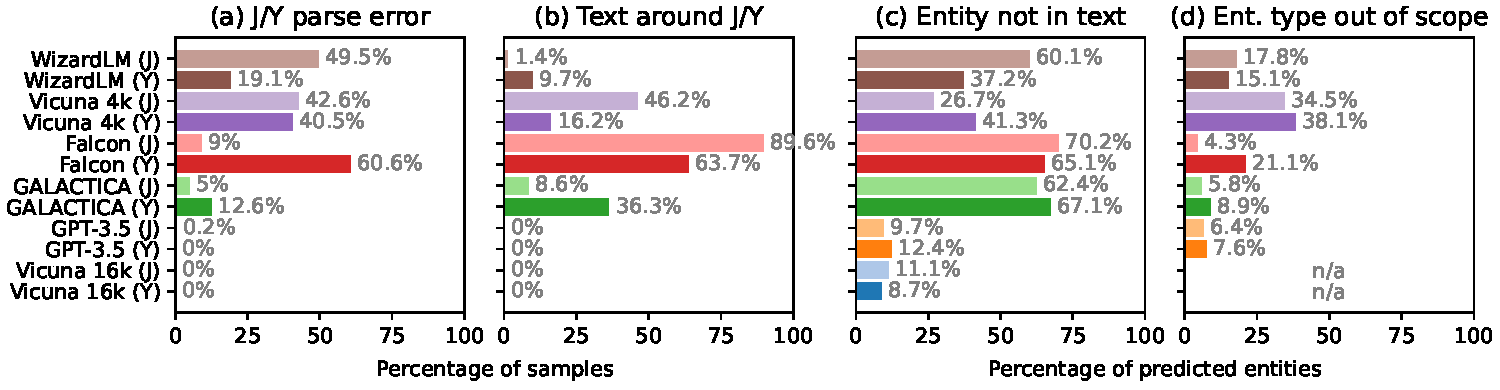
\includegraphics[width=\linewidth]{figures/ref_params/format_eval_mix}
  \caption[Parsing success, format adherence, hallucinations, and scope adherence of LLM generated JSON and YAML]{Parsing success, format adherence, hallucinations, and scope adherence of LLM generated JSON (J) and YAML (Y).}
  \label{fig:yamlVSjson}
\end{figure}

In Figure~\ref{fig:yamlVSjson} we show an analysis of the steps leading up to model prediction. Focussing first on the zero-shot models (upper five) we observe the following across the four plots from left to right. (a)~For three of five models, prompting for YAML leads to fewer parsing errors. (b)~Unwanted text around the extracted data is generated more/less by two models each. (c)~Hallucinated entities and (d)~out of scope entities appear overall slightly more often for in YAML compared to JSON. For our few-shot approach (bottom model), we see that the use of a grammar (a, b)~prevents all output format issues. Furthermore (c)~hallucinated entities are reduced. (d)~Out of scope entities can not be evaluated, because our in-context examples lead to frequent omission of type information in the output.

Through manual analysis we identify a common cause for parsing errors in JSON output to be boolean values (e.g. for ``\texttt{text\_\allowbreak contains\_\allowbreak entities:}'') being copied by the LLM as ``true/false'' from the prompt. We furthermore find that ``entities not in the text'' can arise from unsolicited \LaTeX{} parsing by the LLM (e.g. ``\verb|\lambda|'' in text $\rightarrow$ ``$\lambda$'' in YAML). Prompting for \emph{verbatim} parameter/value strings does not mitigate this.
%TODO: would be nice to add some analysis on the output length when using YAML/JSON and some thoughts as to why the one might work better w/ LLMs than the other (e.g.: YAML is shorter: fewer tokens to "get off track" / JSON mby easier for LLMs to decide when to end b/c of clear brackets instead of just indentation)

% ... a few mentions of quantitative stuff based on format figs.,
% mby look into parsing error msgs

% does not know ``when to stop''

% - saying “LaTeX Input Text” instead of just “Input Text” helped for some models

% automatically changes LaTeX to unicode
% - “\lambda _{\text{C}}” be output as “λC”
%  - not mitigated by changing output “<parameter name>” to “<verbatim parameter name>”


% \subsubsection{Application}
% try to use LLM extracted data as extra training data for supervised model, but observe worse performance

\section{Discussion}\label{sec:discussion}

Our overall results, with a top performance of 79\% $\text{F}_1$ for entity recognition and 39\% $\text{F}_1$ for relation extraction, show that extraction of hyperparameter information from scientific text can be accomplished to a degree that yields sound results. There are, however, challenges that remain, such as more reliable entity recognition of parameters and contexts, as well as more reliable relation extraction in general. Our novel data set enables further development of approaches from hereon. Our IE results on large-scale unannotated data give an indication of possible downstream analyses and applications. Here we see large potential for reproducibility research, faceted search, and recommendation.

Our LLM evaluation shows that for IE tasks dealing with complex information, the choice of text based data serialization format can have a considerable impact on performance, even when using grammar based generation constrains. Additionally, we can see that in-context learning enabled by larger context sizes, as well as grammars, are an effective method to improve IE performance.

\paragraph{Limitations}

(1)~Our work considers HyperPIE from text. This is sensible for a focussed approach, but downstream applications could furthermore benefit from composite pipelines also targeting extraction from tables, source code, etc.
(2)~We do not test transferability of methods to domains outside of ML related fields. It would require domain expertise to find useful definitions for hyperparameters in each respective domain.
(3)~Our LLM evaluation does not cover fine-tuning. Presupposing the existence of a large enough training data set, this would be a valuable addition the overall investigation.
(4)~Defining our YAML/JSON output format hierarchically means that only values associated with parameters and parameters associated with artifacts can be extracted.
(5)~Lastly, our data and experiments unfortunately are limited to English text only and do not cover other languages.

% out of scope LLM predictions: annotation guidelines can be extensive and detailed, therefore hard to ``enforece'' incorporate in in-context learning scenario

% ... focus on limitations of the ``solution'' to the problem presented

% only text, no tables, figures, etc.
% compare with additional fine-tuned models
% investigate hyperparam info as reproducibility indicator more thoroughly
% test transferability of methods (re component to measeval, YAML LLM to mat sci)
% only in English




\section{Conclusion}\label{sec:hyper-conclusion}

%Automatic extraction of information from publication text is key to making scientific knowledge machine-readable at a large scale.
%The extracted information can, for example, facilitate academic search, decision making, and knowledge graph construction.
%An important type of information not covered by existing approaches is hyperparameters.

We formalize the novel ER+RE task HyperPIE and develop approaches for it, thereby expanding IE from scientific text to hyperparameter information. To this end, we create a manually labeled data set spanning various ML fields. In a supervised learning setting, we propose a BERT-based model that achieves an improvement of 29\% $\text{F}_1$ in RE compared to a state-of-the-art baseline. Using the model, we perform IE on a large amount of unannotated papers, and analyze patterns of hyperparameter reporting across ML disciplines. In a zero-/few-shot setting, we propose an LLM based approach using YAML for complex IE, achieving an average improvement of 5.5\% $\text{F}_1$ in ER over using JSON. We furthermore achieve large performance gains for LLMs using grammar based generation constrains and in-context learning. In future work, we plan to investigate fine-tuning LLMs, as well as additional practical use cases for data extracted from large publication corpora, such as knowledge graph construction.

% outlook points
% - try fine-tuning LLMs

% extracted information can be used to extend existing knowledge bases like ORKG or PwC

\section*{Author Contributions}  % see https://credit.niso.org/
Tarek Saier: Conceptualization, Data curation, Formal analysis, Methodology, Software, Visualization, Writing -- original draft, Writing -- review \& editing. Mayumi Ohta: Conceptualization (LLM few-shot), Formal analysis (LLM few-shot), Methodology (LLM few-shot), Software (LLM few-shot), Writing -- original draft (support). Takuto Asakura: Conceptualization, Writing -- review \& editing. Michael F{\"a}rber: Writing -- review \& editing.

%%
%% The acknowledgments section is defined using the "acks" environment
%% (and NOT an unnumbered section). This ensures the proper
%% identification of the section in the article metadata, and the
%% consistent spelling of the heading.
\section*{Acknowledgements}
This work was partially supported by the German Federal Ministry of Education and Research (BMBF) via [KOM,BI], a Software Campus project (01IS17042).
The authors acknowledge support by the state of Baden-W{\"u}rttemberg through bwHPC.
We thank Nicholas Popovic for extensive feedback on the experiment design and prompt engineering. We thank Tarek Gaddour for feedback during the annotation scheme development, and Xiao Ning for input during early model development.

\section{Result Assessment}
\label{sec:hypepie-assessment}

The work in this chapter addresses the following research task.

\begin{rtlist}
    \item[\rtmark{4}:] \textit{Fine-gained Research Artifact Representations} - develop a method to extract fine-grained information on research artifacts from text in scientific publications.
\end{rtlist}

The presented approaches to extracting hyperparameter information from scientific text achieve an improvement in RE compared to a state-of-the-art baseline (39\% compared to 10\% in $\text{F}_1$ score). The applicability of the approach on large-scale data is demonstrated through an analysis of hyperparameter reporting patterns in 15,000 unannotated papers. Previous related approaches, namely SciERC and SciREX, only extract comparably shallow information. Specifically, the parameters and parameters' values of research artifacts are not extracted. Our approach adds this information. Accordingly, we deem \rtmark{4} successfully achieved.

In terms of the overarching research goal of enabling higher-quality scholarly data (see Table~\ref{tab:scholdataquali} in Chapter~\ref{chp:foundations}), the work presented in this chapter makes the following contributions.

\begin{infobox-progress}
      \textbf{Scholarly Data Quality Contributions - \cite{Saier2023hyperpie}}

      \begin{tabular}{lp{10.9cm}}
        \toprule
        Crit. & Contribution \\
        \midrule
        $\mathbf{Rel_{SDR}}$ & Added hyperparameter information to the structured document representations \\
        $\mathbf{Coy_{SDR}}$ & Fine-granular comparison of documents enabled by through artifacts' parameters and their values \\
        \bottomrule
      \end{tabular}
\end{infobox-progress}

$\mathbf{Rel_{SDR}}$ The extracted hyperparameter information from publications' full-text enriches structured document representations with relevant, novel content. Our analysis of hyperparameter reporting patterns in 15,000 papers is a simple demonstration of relevance. Further applications, for which the data is relevant, are, for example, faceted academic search, recommendation, and approaches to automated reproduction.

$\mathbf{Coy_{SDR}}$ The added hyperparameter information enables fine-grained comparison of document contents. For example, sections can be compared or filtered based on whether they contain hyperparameter information or not. Furthermore, comparisons based on parameters and their values are made possible.

% \chapter{References of Joint Use}

\section{Introduction}
\Blindtext[1]

\section{Related Work}
\Blindtext[1]

\section{Approach}
\Blindtext[1]

\section{Evaluation}
\Blindtext[1]

\section{Discussion}
\Blindtext[1]

\chapter{Conclusion}
\label{chp:conclusion}

\section{Summary}

% Structured representations of scientific publications bear large potential for accelerated progress and well-founded strategic decisions in academia. Their use furthermore can mitigate the information overflow that scientists are faced with.
% Our current ``digital record of science'', however, is limited in various ways. This not only prevents faster progress, but also means decisions based on current scholarly data can be flawed and analysis results faulty.
%In pursuit of a remedy, this dissertation set out to alleviate the state of scholarly data. To achieve this, the following research objective was set.
This dissertation set out to alleviate the state of scholarly data. To achieve this, the following research objective was set.

\begin{infobox-objective}
\textbf{Research Objective}\\
Develop an automated process that takes as input scientific publications, and produces as output a high-quality, machine-readable derivative representation of the publications.
\end{infobox-objective}

Criteria for high quality in the context of scholarly data were defined across the following five dimensions.%\footnote{See Table~\ref{tab:scholdataquali} in Chapter~\ref{chp:foundations} for the list of criteria.}

\begin{infobox-progress}
      \textbf{Data Quality Dimensions}\\
       (1)~relevance, (2)~accuracy, (3)~timeliness, (4)~comparability, (5)~completeness
\end{infobox-progress}

For each dimension, criteria were defined for scholarly data's key elements: the citation network (CN) and structured document representations (SDR), as shown in Table~\ref{tab:scholdataquali-again}.

% Based on the way scholarly data is used, the criteria were derived for two focus  areas, the citation network (CN) and structured document representations (SDR), as shown in Table~\ref{tab:scholdataquali-again}. %(see Section~\ref{sec:foundations-dataquality}), 

\begin{table}[tb]
  \caption{Scholarly Data Quality Criteria}
  \label{tab:scholdataquali-again}
  \centering
  \begin{small}
    \begin{threeparttable}
      \begin{tabular}{llll}  % p{9.7cm}
        \toprule
        Dimension & Focus & \multicolumn{2}{l}{Specific Criterion and Short Description} \\
        \midrule
        \multirow{2}{*}{Relevance} & CN & $\mathbf{Rel_{CN}}$ & Representative coverage of publications in area of study \\
        \ & SDR & $\mathbf{Rel_{SDR}}$ & Inclusion of relevant content types (text, math, etc.) \\
        \arrayrulecolor{lightgrey}\hline\arrayrulecolor{black}
        \multirow{2}{*}{Accuracy} & CN & $\mathbf{Acc_{CN}}$ & Correctly linked references \\
        \ & SDR & $\mathbf{Acc_{SDR}}$ & Noise-free full-text content \\
        \arrayrulecolor{lightgrey}\hline\arrayrulecolor{black}
        \multirow{2}{*}{Timeliness} & \multirow{2}{*}{both} & \multirow{2}{*}{$\mathbf{Tim_{C/S}}$} & \multirow{2}{*}{Coverage of recent publications} \\
        \ & \ & \ \\
        \arrayrulecolor{lightgrey}\hline\arrayrulecolor{black}
        \multirow{2}{*}{Comparability} & CN & $\mathbf{Coy_{CN}}$ & Use of established doc. identifiers (DOI, PMID, etc.) \\
        \ & SDR & $\mathbf{Coy_{SDR}}$ & Fine-granular, specifically typed content representation \\
        \arrayrulecolor{lightgrey}\hline\arrayrulecolor{black}
        \multirow{2}{*}{Completeness} & CN & $\mathbf{Cos_{CN}}$ & All references in publications successfully linked \\
        \ & SDR & $\mathbf{Cos_{SDR}}$ & No sections or content missing (appendices, math, etc.) \\
        \bottomrule
      \end{tabular}
      % \begin{tablenotes}
      % \end{tablenotes}
    \end{threeparttable}
  \end{small}
\end{table}

To focus the efforts of improving scholarly data quality, we identified three areas of key importance, in which current scholarly data has significant limitations (see Section \ref{sec:intro-gap}).

\begin{enumerate}
    \item \textbf{Citation Network}\\
          Lacking completeness of the network connecting publications through citations.
    \item \textbf{Anglocentrism}\\
          Lacking coverage of non-English publications in data used and analyzed.
    \item \textbf{Research Artifacts}\\
           Lack of structured representation of research artifacts mentioned in publications.
\end{enumerate}

In order to address these, four research tasks were defined.

\begin{rtlist}
    \item \textit{Base Methodology} - establish a base methodology for generating a large-scale, high-quality scholarly data set, that is on par with or improving upon existing data sets.
    \item \textit{Citation Network Completeness} - develop a method to link literature references, that is able to link more references than are linked in existing data sets, while not compromising on link correctness or processing efficiency.
    \item \textit{Inclusion of Non-English Publications} - find and implement an approach to include non-English publications into a large-scale, high-quality scholarly data set.
    \item \textit{Fine-gained Research Artifact Representations} - develop a method to extract fine-grained information on research artifacts from text in scientific publications.
\end{rtlist}

%To achieve improvements in these areas, the following steps were performed.
The four research tasks were accomplished as follows. % consider s/accomplish/carried out
In Chapter~\ref{chp:corpus}, we developed a corpus creation method transforming publications' \LaTeX{} source files into a large-scale corpus of interlinked, annotated, full-text documents \rtmark{1\large\checkmark}. The presented method also includes a highly accurate reference matching procedure \rtmark{2}{\small(\checkmark)}. Applying our method on the complete set of all publications on arXiv.org, we created the data set \emph{unarXive}, which was used as a basis for all subsequent work. %``Corpus''
In Chapter~\ref{chp:covgran}, we presented improvements regarding the citation network and the granularity of document representations. For the citation network, a blocking technique was developed that, applied on the set of references in a corpus, increases the number of matched references and bibliographic couplings. With an updated corpus creation method, the \emph{unarXive} data set achieved a more complete, state-of-the-art citation network \rtmark{2\large\checkmark}. The updated procedure furthermore enabled more fine-granular document representations, which in turn made the subsequent work in Chapter~\ref{chp:params} possible. %``Reference Coverage and Granularity''
In Chapter~\ref{chp:xling}, we studied cross-lingual citations in the \emph{unarXive} corpus. For this, we developed a method to reliably identify this type of citation based on raw reference strings. In our study, which is the largest of its kind to date, we analysed cross-lingual citations' prevalence, usage, and impact \rtmark{3\large\checkmark}. %``References Across Languages''
Lastly, in Chapter~\ref{chp:params}, we developed methods for extracting information about research artifacts and their usage parameters from publication full-texts. Applying our best performing method on \emph{unarXive}, we found differences in parameter reporting patterns across several disciplines \rtmark{4\large\checkmark}. %``References with Usage Parameters''

Through the accomplishment of the four research tasks, significant improvements across all quality dimensions and criteria were achieved, as summarized in the overview below.

\begin{infobox-progress}
      \textbf{Scholarly Data Quality Contributions - Overview}\vspace{0.5em}

      \begin{tabular}{llcccc}
        \toprule
        Quality Dimension & Criterion\hphantom{mmm}& \multicolumn{4}{c}{Contribution} \\
        \midrule
        \multirow{2}{*}{Relevance} & $\mathbf{Rel_{CN}}$ & {\large\textbf{+}} & = & {\large\textbf{+}} & $\circ$ \\
         & $\mathbf{Rel_{SDR}}$ & $\circ$ & {\large\textbf{+}} & $\circ$ & {\large\textbf{+}} \\
        \arrayrulecolor{lightgrey}\hline\arrayrulecolor{black}
        \multirow{2}{*}{Accuracy} & $\mathbf{Acc_{CN}}$ & {\large\textbf{+}} & = & $\circ$ & $\circ$ \\
         & $\mathbf{Acc_{SDR}}$ & {\large\textbf{+}} & = & $\circ$ & $\circ$ \\
        \arrayrulecolor{lightgrey}\hline\arrayrulecolor{black}
        Timeliness & $\mathbf{Tim_{C/S}}$ & {\large\textbf{+}} & {\large\textbf{+}} & $\circ$ & $\circ$ \\
        \arrayrulecolor{lightgrey}\hline\arrayrulecolor{black}
        \multirow{2}{*}{Comparability} & $\mathbf{Coy_{CN}}$ & {\large\textbf{+}} & {\large\textbf{+}} & {\large\textbf{+}} & $\circ$ \\
         & $\mathbf{Coy_{SDR}}$ & $\circ$ & {\large\textbf{+}} & $\circ$ & {\large\textbf{+}} \\
        \arrayrulecolor{lightgrey}\hline\arrayrulecolor{black}
        \multirow{2}{*}{Completeness} & $\mathbf{Cos_{CN}}$ & {\large\textbf{+}} & {\large\textbf{+}} & $\circ$ & $\circ$ \\
         & $\mathbf{Cos_{SDR}}$ & {\large\textbf{+}} & {\large\textbf{+}} & $\circ$ & $\circ$ \\
        \midrule
        \midrule
        \multicolumn{2}{r}{Chapter} & \ref{chp:corpus} & \ref{chp:covgran} & \ref{chp:xling} & \ref{chp:params} \\
        \multicolumn{2}{r}{Publication} & \cite{Saier2020} & \cite{Saier2022ULITE,Saier2023unarXive} & \cite{Saier2020xling,Saier2021} & \cite{Saier2023hyperpie} \\
        \bottomrule
      \end{tabular}

      \vspace{0.5em}
      \begin{footnotesize}
      \textbf{Legend}\\
      \textbf{+}: SOTA/improvement/etc. (see respective chapter)\\
      =: equal to previous\\
      $\circ$: not considered
      \end{footnotesize}
\end{infobox-progress}

In summary, we successfully addressed three key areas of limitation of current scholarly data and achieved comprehensive improvements in data quality. All introduced methods operate automatically and are demonstrably applicable to large-scale data. %Taking scientific publications as input, our methods generate structured representations.
Accordingly, we argue to have succeeded in developing an automated process producing high-quality derivative representation of scientific publications, and therefore accomplished our \textbf{{\color{objblue-box}\faCrosshairs}\,Research Objective \large\checkmark}

Naturally, advances uncover new challenges, and room for improvement remains. In the following section, we therefore discuss the impact and limitations of our work, as well as prospective avenues for further improvement.

%Details regarding each of the contributions are given in the respective chapters. A discussion of the achieved improvements as well as their limitations can be found in the following section.

\section{Discussion}

% TODO: add some segue foo (bigger picture, broader view, etc.)
We discuss the contributions made in this dissertation from three different perspectives: (1)~the identified research gap, (2)~the five quality dimensions, and (3)~the research community.

% \begin{enumerate}
%     \item The identified research gap
%     \item The five quality dimensions
%     \item The research community
% \end{enumerate}

\subsection{Research Gaps}\label{sec:discussion-rgap}
We made significant progress in all three areas of the identified research gap.

\begin{enumerate}
% what
\item \textbf{Citation Network}\\
Achieving state-of-the-art citation network completeness on a large-scale, multi-discipline corpus,
% impact
means we enable analysis results more valid than previously possible, and the training of prediction models grounded more in reality than before.
% good enough?
That being said, our achieved completeness of 44.4\% means that missing citation links in scholarly data remain a problem.
% path forward
We see potential for future improvements in the development of sophisticated inter-reference blocking and matching methods, building upon our work in Chapter~\ref{chp:covgran}.
%
% what
\item \textbf{Anglocentrism}\\
Performing the largest study on citations of non-English publications to date,
% impact
we provide novel insight into a understudied phenomenon, and are able to highlight challenges for the integration of scholarly data across language borders.
% good enough? / path forward
Based on our findings, we see potential for improvements through better language support of platforms, and more widespread use of unique document identifiers. Another important aspect is the development of information extraction approaches applicable to non-English publications, which our work does not cover.
%
% what
\item \textbf{Research Artifacts}\\
With our task definition as well as model development and application for the extraction of hyperparameter information,
% impact
we enable the use and study of an important type of content in scientific publications.
% good enough?
Our model performance of 79\% $\text{F}_1$ for entity recognition and 39\% for relation extraction indicates remaining challenges particular regarding the latter.
% path forward
Based on our analysis, we can point to parameter entities as a particularly viable focus for achieving improvements in future endeavors.
\end{enumerate}

\subsection{Quality Dimensions}
Through addressing the identified research gap, our work achieves comprehensive improvements of data quality, as determined across five dimensions.

\begin{enumerate}
\item \textbf{Relevance}\\
Our improvements regarding relevance stem from two areas. (i)~We cover a large extent of documents with clear assignability to a subject of study, thereby facilitating, for example, representative coverage of an area of research. This improvement is by virtue of making use of arXiv as a data source. (ii)~We furthermore enable the extraction and structured representation of significant document contents, such as hyperparameter information. This improvement is independent of the specific data source used.
% “general relevance” ~= lots of data + clear assingability to subjects of study
\item \textbf{Accuracy}\\
Improvements we achieve in document representation accuracy are accomplished by harnessing a partially structured data source. In particular, we perform our work based on papers' \LaTeX{} sources. However, similar source types such as JATS XML and DOCX files bear the same potential. %, which presents an opportunity for future developments.
The citation network accuracy of >96\% that we achieve is already very high, with identified errors being edge cases such as follow-up publications with near identical titles. % mby some addition wrt to recall (CN completeness) trade-off?
\item \textbf{Timeliness}\\
Our improvements in terms of data timeliness are a result of us updating our corpus to include recent publications (e.g. up until the end of the most recent completed year). This level of timeliness is arguably sufficient for the study of and applications based on phenomena that do not change within the span of a year, such as citing behavior or writing conventions (e.g. how hyperparameters are reported). Furthermore, a data set with a fixed set of contents is beneficial for comparison of approaches on the same data. For some applications, however, it is desirable to have data on publications included right with their release. An example for this would be paper recommendation. In such cases a ``living corpus'' that is constantly updated is preferable. % consider stating that this is (technically) possible to realize for ppl if they use our method (begs the question though why we then don't provide a living unarXive + snapshots)
\item \textbf{Comparability}\\
We achieve improvements in comparability primarily based on (i)~determining documents' unique identifiers, and (ii)~providing fine-granular structure in our document content representations. (i)~Regarding document identifiers, DOIs are most established in academia, but a significant portion of publications without DOI exists (e.g. 
%about 14\% of PubMed articles in 2015~\cite{10.1007/s11192-016-2225-6}
measured in 2014 on Web of Science and Scopus at 12\% in life sciences, 15\% in physical \& health sciences, and 23\% in social sciences \& humanities~\cite{Gorraiz2016}).
By providing additional identifiers, we can cover part of those as well. (ii)~As for document content, the typed section and paragraph structure we provide in \textit{unarXive} represents natural semantic units on the intra-document level. On the level of sentences, a wide range of structures of interest can be conceived of. Our choice to focus on hyperparameter information is motivated by considerations of potential impact.
\item \textbf{Completeness}\\
Improvements we achieve in terms of data completeness stem from our reference matching---the results of of which we already discussed in Section~\ref{sec:discussion-rgap} above---, and our \LaTeX{} document conversion methodology. Regarding the latter, we are able to provide some document content in addition to the full-text---namely captions of tables and figures as well as mathematical notation. Tables and figures themselves would be a valuable addition, but require the development of additional extraction mechanisms and were not considered. % q: is it "there" if its contained but not in a structured way? i.e., in a PDF
\end{enumerate}

\subsection{Research Community}
Despite its recency, our work already made an impact on the research fields concerned with scholarly data and the study of publications. Below, we give a brief account of ideas and results from this dissertation permeating into and being used by the research community.

\begin{itemize}
    \item Use of \textbf{methodology}
    \begin{itemize}
        \item In~\cite{Lo2020} Lo et al.\ use our corpus creation methodology for creating the \LaTeX{} subset of their S2ORC data set.
        \item Chen et al.\ build on our reference matching procedure in~\cite{chen2021-scixgen} for the creation of their SciXGen data set.
    \end{itemize}
    \item Use for \textbf{model development and evaluation}
    \begin{itemize}
        \item Meyer et al.\ use our data for the development and evaluation of a citation recommendation model in~\cite{Citcom2021}. %~(\cite{Saier2019,HybridCite2020})
        \item In~\cite{Parisot2022}, Parisot and Zavrel train a novel multi-objective representation learning technique for scientific document retrieval on our data.
        \item With Researcher2Vec, Mochihashi presents a method for researcher profile embeddings in~\cite{Mochihashi2023}, using our data to validate their approach.
        %\item Reference Linking~(\cite{Saier2022ULITE})
    \end{itemize}
    \item Use for \textbf{analyses}
    \begin{itemize}
        \item In~\cite{Veneri2022} Veneri et al.\ use our data to investigate how astronomers cite other research fields.
        \item Xue uses our data to analyse in~\cite{Xue2021} semantic shifts of the contexts in which works are cited. %~(\cite{Saier2020xling,Saier2021})
        \item Meng et al.\ use our data in~\cite{Meng2023} for an analysis of omitted citations of works that have become common knowledge --- so called ``obliteration by incorporation''.
    \end{itemize}
    % \item Use for \textbf{data set integration/extension}
    %\begin{itemize}  % TODO: add if Chen paper is ready in time
    %    \item Link Prediction~(\cite{Saier2023cocon})
    %    %\item NER+RE~(\cite{Saier2023hyperpie})
    %\end{itemize}
\end{itemize}

Comparing our work to existing efforts within the research community which strive to create high-quality scholarly data, we find that our work particularly stands out through the \emph{combination} of the following three aspects. (1)~Accurate, fine-granular document representations, (2)~a citation network, and (3)~applicability on a large scale due to being automated. This distinguishes our work from existing efforts as follows. S2ORC~\cite{Lo2020} predominantly uses PDF data and therefore does not provide the same level of granularity (e.g. mathematical notation) and is more prone to noise. arXMLiv~\cite{arXMLiv}, while providing accurate, fine-granular document representations, lacks a citation network. Lastly, the Open Research Knowledge Graph (ORKG)~\cite{orkg1,orkg2} relies on manual or only semi-automated adding of data, and is therefore limited in scale.

% TODO: consider discussing arXiv being a preprint server and the level of difference between preprints on arXiv and their published counterpart

% Note that in other contexts the term ``scholarly data'' can have a broader meaning than just ``structured representations of scientific publications''. For example, it can also include data on research institutions or funding bodies, without necessitating the context of a publication.

%Besides the work described above, there are also efforts of different nature striving towards the same goal. Our and aforementioned similar work seek to represent scientific publications in a broad way.
Our work, as well as the related work described above, seek to represent scientific publications in a broad way.
That is, multiple scientific disciplines and large time spans are covered, and the structured data reflects multiple aspects such as full-text, citation network, authors, etc. Another approach towards high-quality scholarly data are dedicated efforts in specific areas. An example of such an effort is the OpenCitations Index,\refurl{https://opencitations.net/index}{2023-11-30} focussing solely on citation data. Such an approach, however, necessitates the ability to combine multiple dedicated resources. For example, combining citation data with publication full-texts. This is only possible as far as unique persistent identifiers for all involved entities exist---e.g. DOIs for documents, ORCiDs for authors, and ROR IDs for affiliations~\cite{Meadows2019}. Although use of such identifiers is becoming more and more established~\cite{Gorraiz2016}, 
%\footnote{For example, arXiv.org began automatically assigning DOIs to all submissions in 2022, and Springer Nature trialed mandatory use of ORCiDs in 2018. See \refurlinline{https://blog.arxiv.org/2022/02/17/new-arxiv-articles-are-now-automatically-assigned-dois/}{2023-11-30} and \refurlinline{https://info.orcid.org/orcid-mandate-trial-at-springer-nature/}{2023-11-30}.}
gaps in their coverage mean that, for the moment, a combination of dedicated resources is only of limited use~\cite{Youtie2017,Haak2018}.

To briefly recap, we discussed our contributions and impact (1)~in terms of the addressed research gap, (2)~across the five data quality dimensions, and (3)~in relation to the research community. Overall, our work constitutes a range of measurable and demonstrated advancements, and has furthermore been taken up by the research community.

% shown the benefits of using a partially structured data source (\LaTeX{}, JATS XML, DOCX) --- q: is this really a core thing that warrants mentioning in such a prominent position here?

\section{Outlook}

We conclude with a brief look at viable extensions of our work, as well as potential future developments in scientific publishing and what they would mean for the presented work.

\subsection{Extensions of Our Work}

% extension to more input formats
\paragraph{Extension to Other Input Formats}
Our work takes publications' \LaTeX{} source files from arXiv.org as the starting point. Because \LaTeX{} provides a certain level of explicit document structure and semantic information, a natural extension would be to replicate our work on the likewise structured JATS XML publications of the PubMed Central Open Access Subset. This would widen the scope of the results attained, namely by adding life sciences to the already covered disciplines of physics, mathematics, and computer science. In disciplines other than the aforementioned, however, only PDFs are available in large quantities, given the current state of scientific publishing. An extension to PDF input would likely come with challenges regarding structured document representations. However, the work we presented for the focus areas \emph{citation network}, \emph{non-English content}, and \emph{research artifacts}---see Chapters~\ref{chp:covgran}, \ref{chp:xling} and \ref{chp:params} respectively---is not reliant on \LaTeX{} as a starting point. This means, given methods for information extraction from PDFs producing output equal to our intermediate results from \LaTeX{}, extending our work to PDF based document collections is likely possible without major challenges.

\paragraph{Reference Parsing and Matching}
% - recall eval problem (boundless domain)
% - improves w/ continued adaption of DOI use (+DOI aware (+embedded link aware as ours) linking method)
%
% - better ref str parsing (DL, mention igor ppr) + preprocessing (embedded link aware as ours, etc.)
% - better clustering methods
% - increased DOI usage
We achieve state-of-the-art citation network completeness, but the amount of missing citation links in scholarly data remains an issue. Regarding future development, we see three key elements playing a role. First, the parsing of reference strings in order to extract structured information (title, authors, etc.) bears potential for improvement using synthetic training data~\cite{Shapiro2022}. Second, based on our work on reference clustering presented in Chapter~\ref{chp:covgran}, the development and application of novel clustering approaches is promising. Third, a continuation of the trend that DOIs usage is becoming more and more established~\cite{Gorraiz2016} can be expected to simplify the underlying challenge itself, at least regarding future publications.

\paragraph{Integration of Non-English Publication Repositories}
We studied references \emph{to non-English publications} in the English full-text documents in our corpus. More extensive follow-up studies could be made possible by integrating large repositories of non-English publications, such as the Japanese J-STAGE\refurl{https://www.jstage.jst.go.jp/}{2024-02-07} containing over 5 million open access articles. This would enable, for example, studying the ``reverse'' phenomenon of what we examined, and analyse references \emph{from non-English} publications. Furthermore, the resulting large-scale multilingual full-text corpus would be a valuable resource for the development and evaluation of information extraction models not limited to English, thereby further counteracting Anglocentrism in scholarly data related research.

\paragraph{Utilization of Hyperparameter Information}
We developed models for the extraction of hyperparameter information from papers' full-text. To demonstrate their applicability on large-scale data, we perform an exemplary analysis of differences in hyperparameter reporting patterns across disciplines. Beyond this exemplary use, the extracted information bears potential for powering faceted academic search and recommendation systems, as well as the development of approaches to automated reproduction. However, because the performance of our models is still limited, especially in terms of relations extraction when parameter type entities are involved, we see further efforts towards model improvement as a priority.

%\vspace{1em}[Insert visionary paragraph; ``where the journey goes'' considering the above (more multi-discipline, multi-lingual, fine-granular structured information on artifacts etc.). Paint a picture of a possible future.]

\subsection{Future External Developments}

\paragraph{LLMs}
Regarding information extraction methodologies, a continuation of the recent advances in LLM technology could become a key factor in bridging the gap between our by-human for-human publications, and machine-readable scholarly data.
This is because, even though LLM performance is not on par with dedicated models yet~\cite{Yang2023}, the wide-ranging information available to them could allow filling in the assumed background knowledge that is necessary for understanding, but not explicitly mentioned in, scientific publications.
However, a particular challenge with the use of LLMs for the creation of scholarly data, is scaling approaches to large-scale data, because of the required computing resources.

% the future of input formats
\paragraph{Tagged PDFs}
Looking beyond the current state of scholarly data, where it is necessary to apply information extraction methods to retroactively determine document structure and semantic information, future developments concerning ``tagged PDFs''~\cite{Lazar2017} could simplify the creation of high-quality scholarly data. Widespread adoption of encouragement or requirements for semantically tagging PDFs could either be driven by efforts to improve the accessibility of scientific publications, or by the fact that it would facility data mining. In STEM fields, a prerequisite for such a developments would be that the \LaTeX{} Project's plan to support semantic annotation natively succeeds~\cite{Mittelbach2020,Mittelbach2023}.

% the future of publishing
\paragraph{What Constitutes a Publication}
Considering future developments of the landscape of scientific publications, changes to the status quo of papers being the primary unit of publication would accordingly bring changes to the nature of scholarly data. For example, establishment of micropublications~\cite{Raciti2018} and further adoption of data citations~\cite{Kratz2015} could bring new requirements and opportunities to scholarly data, both in terms of data modeling as well as information extraction methods.

\vspace{1em}Through the continuation of our work and that of our colleagues,
we envision a gradual closing of the gap between scientific publications and their machine-readable representation in the form of scholarly data, eventually enabling a digital record of science faithful to its anthropocentric origin.
% - - - choose your level of modesty - - -
% minor
% small
% modest
% tentative
% reasonable
% positive
% noteworthy
% notable
% purposeful
% significant
% meaningful
% substantial
% decisive
% major
% impactful
% pivotal
% vital
% paramount
% critical
% crucial
% indispensable
% foundational
% transformative
% groundbreaking
% monumental
% - - - - - - - - - - - - - - - - - - - -
This dissertation marks a substantial step along this path.


%% Add entry to the table of contents for the bibliography
%\begin{refcontext}[sorting=presorted]
\printbibliography[keyword=own,heading=bibintoc,title={Bibliography of Publications}]
%\end{refcontext}
\printbibliography[notkeyword=own,heading=bibintoc,title={Bibliography of References}]

%% --------------------------------
%% | Appendix                     |
%% --------------------------------
\appendix
\chapter{Appendix}

\section{Geographic origin of all cited non-English languages}\label{app:geo_origin}

In Figure~\ref{fig:geo_full} we show the geographic origin of cross-lingual citations in relative terms per cited language (i.e., the numbers of each \emph{row} add up to 1). The distinct diagonal of the matrix and the horizontal line for affiliations in English speaking countries reflect the fact that most cross-lingual citations are either to a local language or originate from an English speaking country. Among cited languages with a low number of total occurrences we can furthermore see a few cases showing unusual distributions, such as a single citation to Macedonian from an author affiliated with a Polish institution, or citations to Icelandic, where a single one originates from Iceland, while the remaining nine originate from institutions in countries where Japanese (3), Italian (1), and Swedish (5) are the most common language.

\begin{figure*}[tb]
\centering
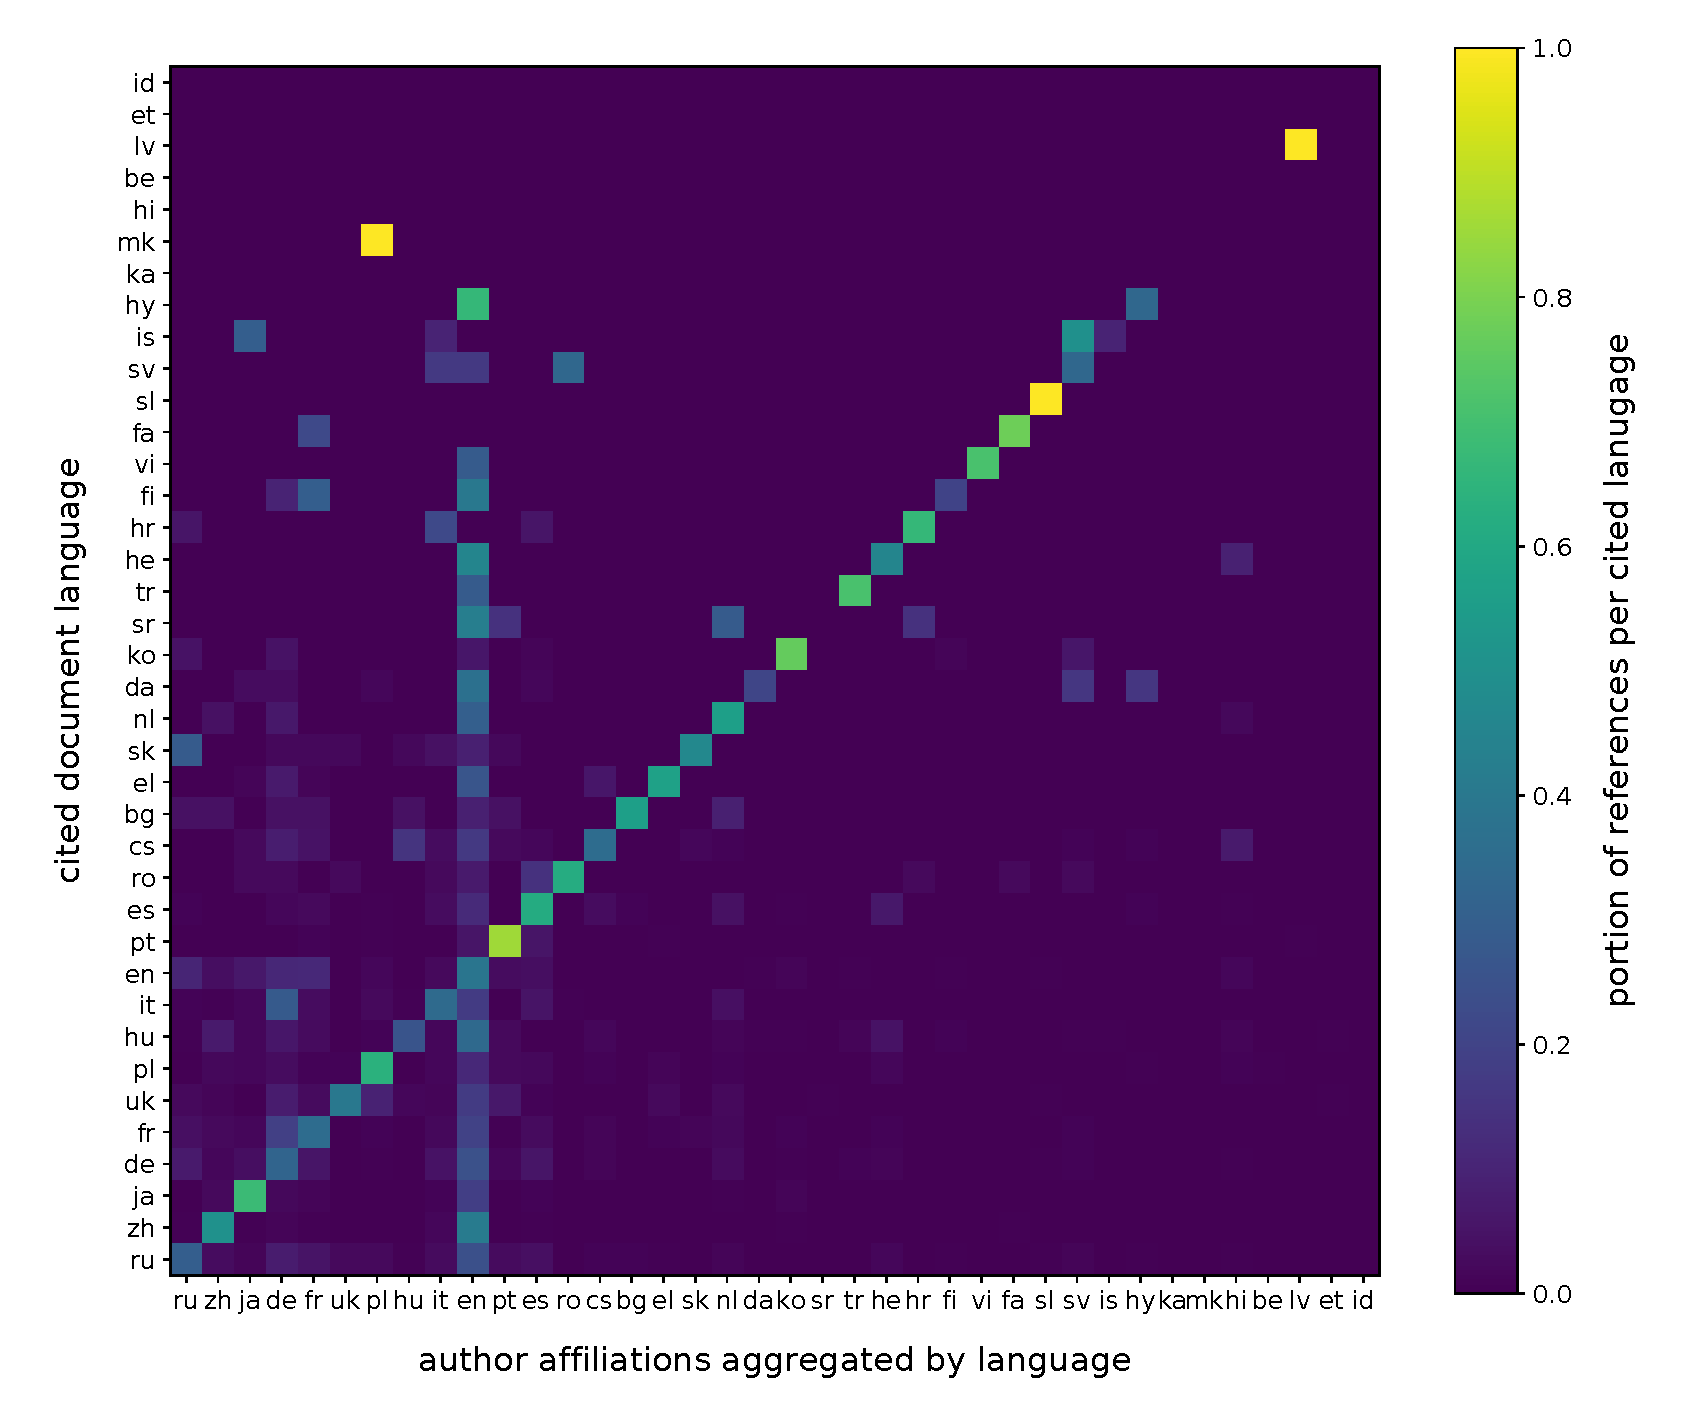
\includegraphics[width=\textwidth]{figures/ref_xling/citlang_to_author_aff_all_relative_crop.pdf}
\caption{Geographic origin of cross-lingual citations (relative count).} \label{fig:geo_full}
\end{figure*}

\section{Citation Intent and Sentiment Classification}\label{app:classifcation}

For the model training of both citation intent classification and citation sentiment classification, we fine-tune SciBERT uncased\footnote{See \url{https://huggingface.co/allenai/scibert_scivocab_uncased}.} using the following model configuration shown in Table~\ref{tab:modelconf}.

\begin{table}
\caption{Model configuration used for training}
 \label{tab:modelconf}
  \centering
  \begin{small}
 \begin{threeparttable}
 \begin{tabular}{lr}
 \toprule
   Hyperparameter & value \\
   \midrule
  attention\_probs\_dropout\_prob &  0.1 \\
  gradient\_checkpointing &  false \\
  hidden\_act &  gelu \\
  hidden\_dropout\_prob &  0.1 \\
  hidden\_size &  768 \\
  initializer\_range &  0.02 \\
  intermediate\_size &  3072 \\
  layer\_norm\_eps &  1e-12 \\
  max\_position\_embeddings &  512 \\
  model\_type &  bert \\
  num\_attention\_heads &  12 \\
  num\_hidden\_layers &  12 \\
  pad\_token\_id &  0 \\
  position\_embedding\_type &  absolute \\
  transformers\_version &  4.4.2 \\
  type\_vocab\_size &  2 \\
  use\_cache &  true \\
  vocab\_size &  31090 \\
   \bottomrule
 \end{tabular}
\end{threeparttable}
  \end{small}
\end{table}

For determining the citation intent, we use the train, validation, and test split provided by the SciCite data set\footnote{See \url{https://huggingface.co/datasets/scicite}.} (train: 74\%, val: 8.3\%, test: 16.9\%). For citation sentiment, we split the Athar data set into train, validation, and test sets into 80\%, 10\%, and 10\%, respectively.



\section{HyperPIE Implementation Details}\label{app:hyperpie-implementation-details}

\paragraph{Fine-Tuned Models:}
We obtain the source code of PL-Marker from the author's GitHub repository\footnote{See \url{https://github.com/thunlp/PL-Marker/}.}. To make it work with our entity and relation schema, we extended the source code in \texttt{run\_acener.py} and \texttt{run\_re.py}. A patch file with all changes is provided in our code share. Our own RE model is a FFNN implemented with 4 hidden layers, each with ReLU activation and dimensions 300, 100, 25 and 2 respectively. All fine-tuned models are trained and evaluated on a local server with a GeForce RTX 3090 (24\,GB).

%  % MLPClassifier(
%  % hidden_layer_sizes=(300, 100, 25, 2),
%  % activation='relu',
%  % solver='adam',
%  % learning_rate_init=0.001,
%  % max_iter=90,
%  % random_state=1,
%  % shuffle=True,
%  % verbose=verbose

\paragraph{LLMs:}
GPT-3.5 was accessed through the official API. The total usage cost for all testing, prompt tuning, and the full evaluation runs sums up to 60\,USD. In zero-shot setting, all open models are run on a high performance compute cluster using the API layer Basaran.\footnote{See \url{https://github.com/hyperonym/basaran/}.} Vicuna and WizardLM  are run on nodes with $4\times$ NVIDIA Tesla V100 (32\,GB). GALACTICA and Falcon are run with half precision on nodes with $4\times$ NVIDIA A100 (80\,GB).

A zero-shot prompt example is shown in Listing~\ref{lst:promptexample}.

\begin{lstlisting}[language=plain,caption=Prompt example.,label=lst:promptexample,breaklines=true,captionpos=b,frame=single,showlines=true,basicstyle=\tiny\ttfamily]
In the context of machine learning and related fields, what (if any) are the entities (datasets, models, methods, loss functions, regularization techniques) mentioned in the LaTeX Input Text below? What (if any) are their parameters and values?

[LaTeX Input Text start]
We use AdamW with a learning rate ($\alpha$) of 1e-3 for /* [...] */
[LaTeX Input Text end]

Answer in the following YAML format.

Format:
---
text_contains_entities: true/false
entities:
  - entity<N>:
      id: e<N>
      name: "<entity name>"
      type: dataset/model/method/loss function/regularization technique
      has_parameters: true/false
      parameters:
        - parameter<M>:
            id: p<N.M>
/* [...] */
...

Only include entities that are of type dataset, model, method, loss function, or regularization technique. Do not output entities that are of another type. Do not include entities of type task, metric, library, software, or API.
Only produce output in the YAML format specified above. Output no additional text.

Output:
\end{lstlisting}

For few-shot prompting, we employed 4\,bit quantization and used the \texttt{llama-cpp-python}\footnote{See \url{https://github.com/abetlen/llama-cpp-python/}.} API. % based on \texttt{llama.cpp}\footnote{See \url{https://github.com/ggerganov/llama.cpp/}.} backend with CUDA multi-GPU acceleration.
We use the default generation setup in \texttt{llama.cpp}
with parameters: temperature = 0, half precision = enabled, and repetition penalty = 1.1. A few-shot prompt example is shown in Listing~\ref{lst:fewshotprompt}.

\begin{lstlisting}[language=plain,caption=Prompt example.,label=lst:fewshotprompt,breaklines=true,captionpos=b,frame=single,showlines=true,basicstyle=\tiny\ttfamily]
### Instruction:
In the context of machine learning and related fields, what (if any) are the entities (datasets, models, methods, loss functions, regularization techniques) mentioned in the LaTeX Input Text below? What (if any) are their parameters and values?

Answer in the following YAML format.

Format:
```
has_entities: true/false
entities:
  - entity<N>:
      id: e<N>
      name: "<entity name>"
      type: dataset/model/method/loss function/regularization technique
      has_parameters: true/false
      parameters:
        - parameter<M>:
            id: p<N.M>
/* [...] */
```

Here are several examples.

### Example 1:

[LaTeX Input Text start]
We use AdamW with a learning rate ($\alpha$) of 1e-3 for /* [...] */
[LaTeX Input Text end]

### Response 1:
```
has_entities: true
  - entity1:
  	  id: e1
      name: "AdamW"
      has_parameters: true
      parameters:
        - parameter1:
            id: p1
/* [...] */
```

### Example 2:

[LaTeX Input Text start]
/* [...] */
[LaTeX Input Text end]

### Response 2:
```
/* [...] */
```

### Example 3:

[LaTeX Input Text start]
/* [...] */
[LaTeX Input Text end]

### Response 3:
```
/* [...] */
```

Only include entities that are of type dataset, model, method, loss function, or regularization technique. Do not output entities that are of another type. Do not include entities of type task, metric, library, software, or API.
Only produce output in the YAML format specified above. Output no additional text.

[LaTeX Input Text start]
We use AdamW with a learning rate ($\alpha$) of 1e-3 for /* [...] */
[LaTeX Input Text end]

### Response:
```
\end{lstlisting}

In the examples given in the few-shot prompts, we omitted the field \texttt{type: dataset/\allowbreak model/\allowbreak method/\allowbreak loss function/\allowbreak regularization technique}, because this information is not part of the gold annotation. As a consequence, the model outputs also tend to skip this attribute.

% \chapter{Bappendix}

% \section{Bar}
% \Blindtext


\end{document}
